% Options for packages loaded elsewhere
\PassOptionsToPackage{unicode}{hyperref}
\PassOptionsToPackage{hyphens}{url}
%
\documentclass[
]{book}
\usepackage{lmodern}
\usepackage{amssymb,amsmath}
\usepackage{ifxetex,ifluatex}
\ifnum 0\ifxetex 1\fi\ifluatex 1\fi=0 % if pdftex
  \usepackage[T1]{fontenc}
  \usepackage[utf8]{inputenc}
  \usepackage{textcomp} % provide euro and other symbols
\else % if luatex or xetex
  \usepackage{unicode-math}
  \defaultfontfeatures{Scale=MatchLowercase}
  \defaultfontfeatures[\rmfamily]{Ligatures=TeX,Scale=1}
\fi
% Use upquote if available, for straight quotes in verbatim environments
\IfFileExists{upquote.sty}{\usepackage{upquote}}{}
\IfFileExists{microtype.sty}{% use microtype if available
  \usepackage[]{microtype}
  \UseMicrotypeSet[protrusion]{basicmath} % disable protrusion for tt fonts
}{}
\makeatletter
\@ifundefined{KOMAClassName}{% if non-KOMA class
  \IfFileExists{parskip.sty}{%
    \usepackage{parskip}
  }{% else
    \setlength{\parindent}{0pt}
    \setlength{\parskip}{6pt plus 2pt minus 1pt}}
}{% if KOMA class
  \KOMAoptions{parskip=half}}
\makeatother
\usepackage{xcolor}
\IfFileExists{xurl.sty}{\usepackage{xurl}}{} % add URL line breaks if available
\IfFileExists{bookmark.sty}{\usepackage{bookmark}}{\usepackage{hyperref}}
\hypersetup{
  pdftitle={COVID dataset analyzing},
  pdfauthor={Cristina Díaz García, Beatriz Huertas Calvillo, Miguel Lillo del Barrio, María Vázquez Pendón},
  hidelinks,
  pdfcreator={LaTeX via pandoc}}
\urlstyle{same} % disable monospaced font for URLs
\usepackage{color}
\usepackage{fancyvrb}
\newcommand{\VerbBar}{|}
\newcommand{\VERB}{\Verb[commandchars=\\\{\}]}
\DefineVerbatimEnvironment{Highlighting}{Verbatim}{commandchars=\\\{\}}
% Add ',fontsize=\small' for more characters per line
\usepackage{framed}
\definecolor{shadecolor}{RGB}{248,248,248}
\newenvironment{Shaded}{\begin{snugshade}}{\end{snugshade}}
\newcommand{\AlertTok}[1]{\textcolor[rgb]{0.94,0.16,0.16}{#1}}
\newcommand{\AnnotationTok}[1]{\textcolor[rgb]{0.56,0.35,0.01}{\textbf{\textit{#1}}}}
\newcommand{\AttributeTok}[1]{\textcolor[rgb]{0.77,0.63,0.00}{#1}}
\newcommand{\BaseNTok}[1]{\textcolor[rgb]{0.00,0.00,0.81}{#1}}
\newcommand{\BuiltInTok}[1]{#1}
\newcommand{\CharTok}[1]{\textcolor[rgb]{0.31,0.60,0.02}{#1}}
\newcommand{\CommentTok}[1]{\textcolor[rgb]{0.56,0.35,0.01}{\textit{#1}}}
\newcommand{\CommentVarTok}[1]{\textcolor[rgb]{0.56,0.35,0.01}{\textbf{\textit{#1}}}}
\newcommand{\ConstantTok}[1]{\textcolor[rgb]{0.00,0.00,0.00}{#1}}
\newcommand{\ControlFlowTok}[1]{\textcolor[rgb]{0.13,0.29,0.53}{\textbf{#1}}}
\newcommand{\DataTypeTok}[1]{\textcolor[rgb]{0.13,0.29,0.53}{#1}}
\newcommand{\DecValTok}[1]{\textcolor[rgb]{0.00,0.00,0.81}{#1}}
\newcommand{\DocumentationTok}[1]{\textcolor[rgb]{0.56,0.35,0.01}{\textbf{\textit{#1}}}}
\newcommand{\ErrorTok}[1]{\textcolor[rgb]{0.64,0.00,0.00}{\textbf{#1}}}
\newcommand{\ExtensionTok}[1]{#1}
\newcommand{\FloatTok}[1]{\textcolor[rgb]{0.00,0.00,0.81}{#1}}
\newcommand{\FunctionTok}[1]{\textcolor[rgb]{0.00,0.00,0.00}{#1}}
\newcommand{\ImportTok}[1]{#1}
\newcommand{\InformationTok}[1]{\textcolor[rgb]{0.56,0.35,0.01}{\textbf{\textit{#1}}}}
\newcommand{\KeywordTok}[1]{\textcolor[rgb]{0.13,0.29,0.53}{\textbf{#1}}}
\newcommand{\NormalTok}[1]{#1}
\newcommand{\OperatorTok}[1]{\textcolor[rgb]{0.81,0.36,0.00}{\textbf{#1}}}
\newcommand{\OtherTok}[1]{\textcolor[rgb]{0.56,0.35,0.01}{#1}}
\newcommand{\PreprocessorTok}[1]{\textcolor[rgb]{0.56,0.35,0.01}{\textit{#1}}}
\newcommand{\RegionMarkerTok}[1]{#1}
\newcommand{\SpecialCharTok}[1]{\textcolor[rgb]{0.00,0.00,0.00}{#1}}
\newcommand{\SpecialStringTok}[1]{\textcolor[rgb]{0.31,0.60,0.02}{#1}}
\newcommand{\StringTok}[1]{\textcolor[rgb]{0.31,0.60,0.02}{#1}}
\newcommand{\VariableTok}[1]{\textcolor[rgb]{0.00,0.00,0.00}{#1}}
\newcommand{\VerbatimStringTok}[1]{\textcolor[rgb]{0.31,0.60,0.02}{#1}}
\newcommand{\WarningTok}[1]{\textcolor[rgb]{0.56,0.35,0.01}{\textbf{\textit{#1}}}}
\usepackage{longtable,booktabs}
% Correct order of tables after \paragraph or \subparagraph
\usepackage{etoolbox}
\makeatletter
\patchcmd\longtable{\par}{\if@noskipsec\mbox{}\fi\par}{}{}
\makeatother
% Allow footnotes in longtable head/foot
\IfFileExists{footnotehyper.sty}{\usepackage{footnotehyper}}{\usepackage{footnote}}
\makesavenoteenv{longtable}
\usepackage{graphicx}
\makeatletter
\def\maxwidth{\ifdim\Gin@nat@width>\linewidth\linewidth\else\Gin@nat@width\fi}
\def\maxheight{\ifdim\Gin@nat@height>\textheight\textheight\else\Gin@nat@height\fi}
\makeatother
% Scale images if necessary, so that they will not overflow the page
% margins by default, and it is still possible to overwrite the defaults
% using explicit options in \includegraphics[width, height, ...]{}
\setkeys{Gin}{width=\maxwidth,height=\maxheight,keepaspectratio}
% Set default figure placement to htbp
\makeatletter
\def\fps@figure{htbp}
\makeatother
\setlength{\emergencystretch}{3em} % prevent overfull lines
\providecommand{\tightlist}{%
  \setlength{\itemsep}{0pt}\setlength{\parskip}{0pt}}
\setcounter{secnumdepth}{5}
\usepackage{booktabs}
\usepackage{amsthm}
\makeatletter
\def\thm@space@setup{%
  \thm@preskip=8pt plus 2pt minus 4pt
  \thm@postskip=\thm@preskip
}
\makeatother
\usepackage[]{natbib}
\bibliographystyle{apalike}

\title{COVID dataset analyzing}
\author{Cristina Díaz García, Beatriz Huertas Calvillo, Miguel Lillo del Barrio, María Vázquez Pendón}
\date{2020-06-28}

\begin{document}
\maketitle

{
\setcounter{tocdepth}{1}
\tableofcontents
}
\hypertarget{description}{%
\chapter*{Description}\label{description}}
\addcontentsline{toc}{chapter}{Description}

This is an analysis of a COVID dataset using different approaches.

\hypertarget{visualization}{%
\chapter{Visualization}\label{visualization}}

\hypertarget{death-and-healed-calendar}{%
\section{Death and Healed Calendar}\label{death-and-healed-calendar}}

\begin{Shaded}
\begin{Highlighting}[]
\KeywordTok{library}\NormalTok{(readxl)}
\KeywordTok{library}\NormalTok{(dplyr)}
\KeywordTok{library}\NormalTok{(ggplot2)}
\KeywordTok{library}\NormalTok{(lubridate)}
\KeywordTok{library}\NormalTok{(openair)}
\KeywordTok{library}\NormalTok{(lattice)}
\NormalTok{cs\_export \textless{}{-}}\StringTok{ }\KeywordTok{read\_excel}\NormalTok{(}\StringTok{"cs\_export.xls"}\NormalTok{)}
\NormalTok{filasandalucia \textless{}{-}}\StringTok{ }\KeywordTok{filter}\NormalTok{(cs\_export, Territorio}\OperatorTok{==}\StringTok{"Andalucía"}\NormalTok{ )}
\CommentTok{\#View(filasandalucia)}
\KeywordTok{colnames}\NormalTok{(filasandalucia)[}\DecValTok{1}\NormalTok{] \textless{}{-}}\StringTok{ "fecha"}
\CommentTok{\#\#Calendario defunciones}
\NormalTok{filasandalucia}\OperatorTok{$}\NormalTok{fecha \textless{}{-}}\StringTok{ }\KeywordTok{as.factor}\NormalTok{(filasandalucia}\OperatorTok{$}\NormalTok{fecha)}
\KeywordTok{class}\NormalTok{(filasandalucia}\OperatorTok{$}\NormalTok{fecha)}
\end{Highlighting}
\end{Shaded}

\begin{verbatim}
## [1] "factor"
\end{verbatim}

\begin{Shaded}
\begin{Highlighting}[]
\NormalTok{datos \textless{}{-}}\StringTok{ }\NormalTok{filasandalucia }\OperatorTok{\%\textgreater{}\%}\StringTok{ }\NormalTok{dplyr}\OperatorTok{::}\KeywordTok{select}\NormalTok{(}\DataTypeTok{date =}\NormalTok{ fecha, Defunciones) }\OperatorTok{\%\textgreater{}\%}\StringTok{ }\KeywordTok{mutate}\NormalTok{(}\DataTypeTok{date =} \KeywordTok{as.Date}\NormalTok{(date,}\DataTypeTok{format=}\StringTok{"\%d/\%m/\%Y"}\NormalTok{)) }\OperatorTok{\%\textgreater{}\%}\StringTok{ }
\StringTok{  }\CommentTok{\# Quitar febrero}
\StringTok{  }\KeywordTok{filter}\NormalTok{(}\KeywordTok{month}\NormalTok{(date) }\OperatorTok{!=}\StringTok{ }\DecValTok{2}\NormalTok{)}
\NormalTok{datos \textless{}{-}}\StringTok{ }\KeywordTok{as.data.frame}\NormalTok{(datos)}
\CommentTok{\# Guardar calendario}
\CommentTok{\#png("14.png", width = 10, height = 3.5, units = "in", res = 300)}
\KeywordTok{calendarPlot}\NormalTok{(datos,}
             \DataTypeTok{pollutant =} \StringTok{"Defunciones"}\NormalTok{,}
             \CommentTok{\# Título}
             \DataTypeTok{main =} \StringTok{"Defunciones diarias por coronavirus en Andalucía }\CharTok{\textbackslash{}n}\StringTok{Marzo{-}Mayo, 2020"}\NormalTok{,}
             \CommentTok{\# Para que el calendario empiece en lunes}
             \DataTypeTok{w.shift =} \DecValTok{2}\NormalTok{,}
             \DataTypeTok{limits =} \KeywordTok{c}\NormalTok{(}\DecValTok{0}\NormalTok{, }\KeywordTok{max}\NormalTok{(datos}\OperatorTok{$}\NormalTok{Defunciones)),}
             \CommentTok{\# Colores para los eventos (del 0 al 3)}
             \DataTypeTok{cols =} \KeywordTok{c}\NormalTok{(}\StringTok{"white"}\NormalTok{, }\StringTok{"darkred"}\NormalTok{),}
             \DataTypeTok{key.header =} \StringTok{"Defunciones diarias"}\NormalTok{)}
\end{Highlighting}
\end{Shaded}

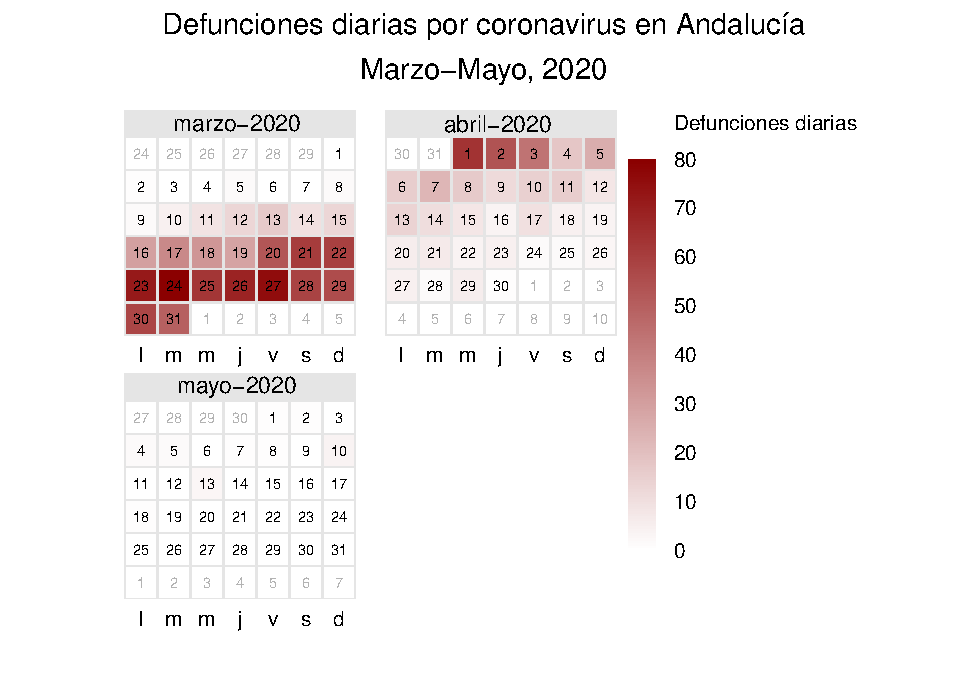
\includegraphics{bookdown-demo_files/figure-latex/unnamed-chunk-1-1.pdf}

\begin{Shaded}
\begin{Highlighting}[]
\CommentTok{\#dev.off()}
\CommentTok{\#\# Calendario curados}
\NormalTok{datos \textless{}{-}}\StringTok{ }\NormalTok{filasandalucia }\OperatorTok{\%\textgreater{}\%}\StringTok{ }
\StringTok{  }\NormalTok{dplyr}\OperatorTok{::}\KeywordTok{select}\NormalTok{(}\DataTypeTok{date =}\NormalTok{ fecha, Curados) }\OperatorTok{\%\textgreater{}\%}\StringTok{ }
\StringTok{  }\KeywordTok{mutate}\NormalTok{(}\DataTypeTok{date =} \KeywordTok{as.Date}\NormalTok{(date,}\DataTypeTok{format=}\StringTok{"\%d/\%m/\%Y"}\NormalTok{)) }\OperatorTok{\%\textgreater{}\%}\StringTok{ }
\StringTok{  }\CommentTok{\# Quitar febrero}
\StringTok{  }\KeywordTok{filter}\NormalTok{(}\KeywordTok{month}\NormalTok{(date) }\OperatorTok{!=}\StringTok{ }\DecValTok{2}\NormalTok{)}
\NormalTok{datos \textless{}{-}}\StringTok{ }\KeywordTok{as.data.frame}\NormalTok{(datos)}
\CommentTok{\#png("15.png", width = 10, height = 3.5, units = "in", res = 300)}
\KeywordTok{calendarPlot}\NormalTok{(datos,}
             \DataTypeTok{pollutant =} \StringTok{"Curados"}\NormalTok{,}
             \CommentTok{\# Título}
             \DataTypeTok{main =} \StringTok{"Curados cada día de coronavirus en Andalucía }\CharTok{\textbackslash{}n}\StringTok{Marzo{-}Mayo, 2020"}\NormalTok{,}
             \CommentTok{\# Para que el calendario empiece en lunes}
             \DataTypeTok{w.shift =} \DecValTok{2}\NormalTok{,}
             \DataTypeTok{limits =} \KeywordTok{c}\NormalTok{(}\DecValTok{0}\NormalTok{, }\KeywordTok{max}\NormalTok{(datos}\OperatorTok{$}\NormalTok{Curados)),}
             \CommentTok{\# Colores para los eventos (del 0 al 3)}
             \DataTypeTok{cols =} \KeywordTok{c}\NormalTok{(}\StringTok{"white"}\NormalTok{, }\StringTok{"darkgreen"}\NormalTok{),}
             \DataTypeTok{key.header =} \StringTok{"Curados cada día"}\NormalTok{)}
\end{Highlighting}
\end{Shaded}

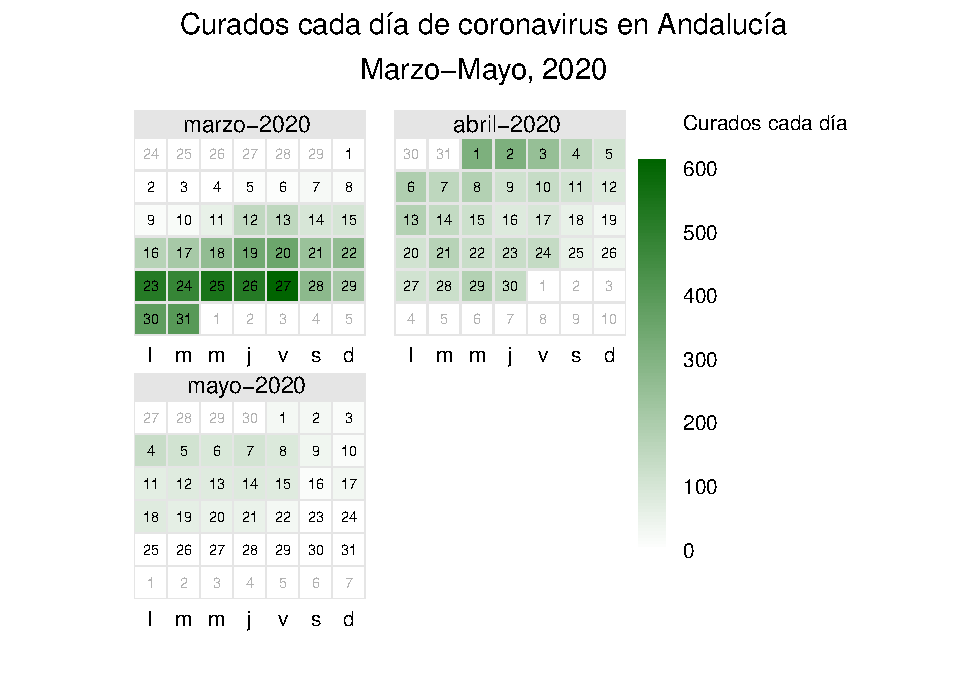
\includegraphics{bookdown-demo_files/figure-latex/unnamed-chunk-1-2.pdf}

\begin{Shaded}
\begin{Highlighting}[]
\CommentTok{\#dev.off()}
\end{Highlighting}
\end{Shaded}

\hypertarget{confirmed-cases-bar-graph}{%
\section{Confirmed cases bar graph}\label{confirmed-cases-bar-graph}}

\begin{Shaded}
\begin{Highlighting}[]
\CommentTok{\# Librerías a utilizar}
\KeywordTok{library}\NormalTok{(tidyverse)}
\KeywordTok{library}\NormalTok{(gganimate)}
\KeywordTok{library}\NormalTok{(readxl)}
\CommentTok{\# Cargo los datos a trabajar}
\NormalTok{cs\_export \textless{}{-}}\StringTok{ }\KeywordTok{read\_excel}\NormalTok{(}\StringTok{"cs\_export.xls"}\NormalTok{) }\OperatorTok{\%\textgreater{}\%}\StringTok{ }\KeywordTok{print}\NormalTok{()}
\end{Highlighting}
\end{Shaded}

\begin{verbatim}
## # A tibble: 687 x 8
##    `Fecha declarac~ Territorio `Confirmados PC~ Hospitalizados   UCI Curados
##    <chr>            <chr>                 <dbl>          <dbl> <dbl>   <dbl>
##  1 22/05/2020       Andalucía                 9              6     0      26
##  2 22/05/2020       Almería                   1              2     0       4
##  3 22/05/2020       Córdoba                   0              0     0       1
##  4 22/05/2020       Granada                   0              1     0      11
##  5 22/05/2020       Huelva                    1              1     0       0
##  6 22/05/2020       Jaén                      5              2     0       1
##  7 22/05/2020       Málaga                    2              0     0       5
##  8 22/05/2020       Sevilla                   0              0     0       4
##  9 21/05/2020       Andalucía                16              5     0      52
## 10 21/05/2020       Almería                   0              0     0       4
## # ... with 677 more rows, and 2 more variables: Defunciones <dbl>, `Total
## #   confirmados (PCR+test)` <dbl>
\end{verbatim}

\begin{Shaded}
\begin{Highlighting}[]
\CommentTok{\# proceso los datos a utlizar}
\NormalTok{confirmados \textless{}{-}}\StringTok{ }
\StringTok{ }\NormalTok{cs\_export }\OperatorTok{\%\textgreater{}\%}\StringTok{ }
\StringTok{  }\KeywordTok{group\_by}\NormalTok{(Territorio, }\StringTok{\textasciigrave{}}\DataTypeTok{Fecha declaración}\StringTok{\textasciigrave{}}\NormalTok{)}\OperatorTok{\%\textgreater{}\%}\StringTok{ }
\StringTok{  }\KeywordTok{print}\NormalTok{()}
\end{Highlighting}
\end{Shaded}

\begin{verbatim}
## # A tibble: 687 x 8
## # Groups:   Territorio, Fecha declaración [686]
##    `Fecha declarac~ Territorio `Confirmados PC~ Hospitalizados   UCI Curados
##    <chr>            <chr>                 <dbl>          <dbl> <dbl>   <dbl>
##  1 22/05/2020       Andalucía                 9              6     0      26
##  2 22/05/2020       Almería                   1              2     0       4
##  3 22/05/2020       Córdoba                   0              0     0       1
##  4 22/05/2020       Granada                   0              1     0      11
##  5 22/05/2020       Huelva                    1              1     0       0
##  6 22/05/2020       Jaén                      5              2     0       1
##  7 22/05/2020       Málaga                    2              0     0       5
##  8 22/05/2020       Sevilla                   0              0     0       4
##  9 21/05/2020       Andalucía                16              5     0      52
## 10 21/05/2020       Almería                   0              0     0       4
## # ... with 677 more rows, and 2 more variables: Defunciones <dbl>, `Total
## #   confirmados (PCR+test)` <dbl>
\end{verbatim}

\begin{Shaded}
\begin{Highlighting}[]
\NormalTok{almeria \textless{}{-}}\StringTok{ }\NormalTok{confirmados }\OperatorTok{\%\textgreater{}\%}\StringTok{ }\KeywordTok{filter}\NormalTok{(Territorio}\OperatorTok{==}\StringTok{"Almería"}\NormalTok{)}
\NormalTok{almeriaacum \textless{}{-}}\StringTok{ }\KeywordTok{colSums}\NormalTok{(almeria[}\DecValTok{3}\OperatorTok{:}\DecValTok{8}\NormalTok{])}
\NormalTok{cadiz \textless{}{-}}\StringTok{ }\NormalTok{confirmados }\OperatorTok{\%\textgreater{}\%}\StringTok{ }\KeywordTok{filter}\NormalTok{(Territorio}\OperatorTok{==}\StringTok{"Cádiz"}\NormalTok{)}
\NormalTok{cadizacum \textless{}{-}}\StringTok{ }\KeywordTok{colSums}\NormalTok{(cadiz[}\DecValTok{3}\OperatorTok{:}\DecValTok{8}\NormalTok{])}
\NormalTok{cordoba \textless{}{-}}\StringTok{ }\NormalTok{confirmados }\OperatorTok{\%\textgreater{}\%}\StringTok{ }\KeywordTok{filter}\NormalTok{(Territorio}\OperatorTok{==}\StringTok{"Córdoba"}\NormalTok{)}
\NormalTok{cordobaacum \textless{}{-}}\StringTok{ }\KeywordTok{colSums}\NormalTok{(cordoba[}\DecValTok{3}\OperatorTok{:}\DecValTok{8}\NormalTok{])}
\NormalTok{granada \textless{}{-}}\StringTok{ }\NormalTok{confirmados }\OperatorTok{\%\textgreater{}\%}\StringTok{ }\KeywordTok{filter}\NormalTok{(Territorio}\OperatorTok{==}\StringTok{"Granada"}\NormalTok{)}
\NormalTok{granadaacum \textless{}{-}}\StringTok{ }\KeywordTok{colSums}\NormalTok{(granada[}\DecValTok{3}\OperatorTok{:}\DecValTok{8}\NormalTok{])}
\NormalTok{huelva \textless{}{-}}\StringTok{ }\NormalTok{confirmados }\OperatorTok{\%\textgreater{}\%}\StringTok{ }\KeywordTok{filter}\NormalTok{(Territorio}\OperatorTok{==}\StringTok{"Huelva"}\NormalTok{)}
\NormalTok{huelvaacum \textless{}{-}}\StringTok{ }\KeywordTok{colSums}\NormalTok{(huelva[}\DecValTok{3}\OperatorTok{:}\DecValTok{8}\NormalTok{])}
\NormalTok{jaen \textless{}{-}}\StringTok{ }\NormalTok{confirmados }\OperatorTok{\%\textgreater{}\%}\StringTok{ }\KeywordTok{filter}\NormalTok{(Territorio}\OperatorTok{==}\StringTok{"Jaén"}\NormalTok{)}
\NormalTok{jaenacum \textless{}{-}}\StringTok{ }\KeywordTok{colSums}\NormalTok{(jaen[}\DecValTok{3}\OperatorTok{:}\DecValTok{8}\NormalTok{])}
\NormalTok{malaga \textless{}{-}}\StringTok{ }\NormalTok{confirmados }\OperatorTok{\%\textgreater{}\%}\StringTok{ }\KeywordTok{filter}\NormalTok{(Territorio}\OperatorTok{==}\StringTok{"Málaga"}\NormalTok{)}
\NormalTok{malagaacum \textless{}{-}}\StringTok{ }\KeywordTok{colSums}\NormalTok{(malaga[}\DecValTok{3}\OperatorTok{:}\DecValTok{8}\NormalTok{])}
\NormalTok{sevilla \textless{}{-}}\StringTok{ }\NormalTok{confirmados }\OperatorTok{\%\textgreater{}\%}\StringTok{ }\KeywordTok{filter}\NormalTok{(Territorio}\OperatorTok{==}\StringTok{"Sevilla"}\NormalTok{)}
\NormalTok{sevillaacum \textless{}{-}}\StringTok{ }\KeywordTok{colSums}\NormalTok{(sevilla[}\DecValTok{3}\OperatorTok{:}\DecValTok{8}\NormalTok{])}
\NormalTok{dfaux \textless{}{-}}\StringTok{ }\KeywordTok{data.frame}\NormalTok{(}\StringTok{"Provincia"}\NormalTok{=}\KeywordTok{c}\NormalTok{(}\StringTok{"Sevilla"}\NormalTok{,}\StringTok{"Málaga"}\NormalTok{,}\StringTok{"Jaén"}\NormalTok{,}\StringTok{"Huelva"}\NormalTok{,}\StringTok{"Granada"}\NormalTok{,}\StringTok{"Córdoba"}\NormalTok{,}\StringTok{"Cádiz"}\NormalTok{,}\StringTok{"Almería"}\NormalTok{),}\StringTok{"ConfirmadosAcum"}\NormalTok{=}\KeywordTok{c}\NormalTok{(sevillaacum[}\DecValTok{6}\NormalTok{],malagaacum[}\DecValTok{6}\NormalTok{],jaenacum[}\DecValTok{6}\NormalTok{],huelvaacum[}\DecValTok{6}\NormalTok{],granadaacum[}\DecValTok{6}\NormalTok{],cordobaacum[}\DecValTok{6}\NormalTok{],cadizacum[}\DecValTok{6}\NormalTok{],almeriaacum[}\DecValTok{6}\NormalTok{]))}
\CommentTok{\# genero el gráfico estático}
\NormalTok{plot\_conf \textless{}{-}}\StringTok{ }
\StringTok{  }\KeywordTok{ggplot}\NormalTok{(dfaux, }
         \KeywordTok{aes}\NormalTok{(}\DataTypeTok{x =}\NormalTok{ dfaux}\OperatorTok{$}\NormalTok{ConfirmadosAcum, }
             \DataTypeTok{y =}\NormalTok{ dfaux}\OperatorTok{$}\NormalTok{Provincia, }
             \DataTypeTok{colour =} \KeywordTok{as.factor}\NormalTok{(dfaux}\OperatorTok{$}\NormalTok{Provincia), }
             \DataTypeTok{fill =} \KeywordTok{as.factor}\NormalTok{(dfaux}\OperatorTok{$}\NormalTok{Provincia))) }\OperatorTok{+}\StringTok{ }
\StringTok{  }\KeywordTok{geom\_bar}\NormalTok{(}\DataTypeTok{stat =} \StringTok{"identity"}\NormalTok{,}\DataTypeTok{position=}\StringTok{"stack"}\NormalTok{) }\OperatorTok{+}\StringTok{ }
\StringTok{  }\KeywordTok{scale\_x\_continuous}\NormalTok{(}\DataTypeTok{breaks =} \KeywordTok{seq}\NormalTok{(}\DecValTok{500}\NormalTok{, }\DecValTok{5000}\NormalTok{, }\DecValTok{500}\NormalTok{), }\DataTypeTok{expand =} \KeywordTok{c}\NormalTok{(}\DecValTok{0}\NormalTok{,}\DecValTok{0}\NormalTok{)) }\OperatorTok{+}\StringTok{ }
\StringTok{  }\KeywordTok{theme\_bw}\NormalTok{() }\OperatorTok{+}\StringTok{ }
\StringTok{  }\KeywordTok{theme}\NormalTok{(}\DataTypeTok{axis.title =} \KeywordTok{element\_blank}\NormalTok{(), }
        \DataTypeTok{axis.ticks.y =} \KeywordTok{element\_blank}\NormalTok{(), }
        \DataTypeTok{legend.position =} \StringTok{"none"}\NormalTok{, }
        \DataTypeTok{panel.grid.minor =} \KeywordTok{element\_blank}\NormalTok{(), }
        \DataTypeTok{panel.grid.major.y =} \KeywordTok{element\_blank}\NormalTok{())}\OperatorTok{+}\KeywordTok{ggtitle}\NormalTok{(}\StringTok{"Casos confirmados mediante tests por provincias"}\NormalTok{)}
\NormalTok{plot\_conf}
\end{Highlighting}
\end{Shaded}

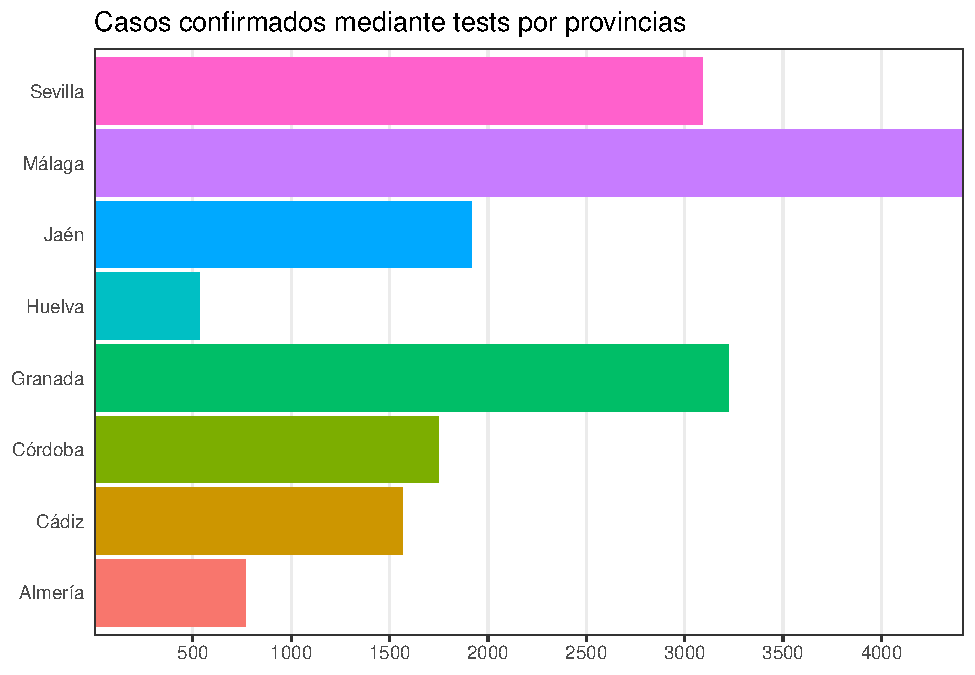
\includegraphics{bookdown-demo_files/figure-latex/unnamed-chunk-2-1.pdf}

\hypertarget{andalusia-bar-graphs}{%
\section{Andalusia bar graphs}\label{andalusia-bar-graphs}}

\begin{Shaded}
\begin{Highlighting}[]
\KeywordTok{library}\NormalTok{(readxl)}
\KeywordTok{library}\NormalTok{(dplyr)}
\KeywordTok{library}\NormalTok{(ggplot2)}
\KeywordTok{library}\NormalTok{(lubridate)}
\KeywordTok{library}\NormalTok{(openair)}
\KeywordTok{library}\NormalTok{(lattice)}
\NormalTok{cs\_export \textless{}{-}}\StringTok{ }\KeywordTok{read\_excel}\NormalTok{(}\StringTok{"cs\_export.xls"}\NormalTok{)}
\NormalTok{filasandalucia \textless{}{-}}\StringTok{ }\KeywordTok{filter}\NormalTok{(cs\_export, Territorio}\OperatorTok{==}\StringTok{"Andalucía"}\NormalTok{ )}
\NormalTok{aux \textless{}{-}}\StringTok{ }\NormalTok{filasandalucia}
\NormalTok{fechas \textless{}{-}}\StringTok{ }\KeywordTok{as.Date}\NormalTok{(aux}\OperatorTok{$}\StringTok{\textasciigrave{}}\DataTypeTok{Fecha declaración}\StringTok{\textasciigrave{}}\NormalTok{,}\StringTok{"\%d/\%m/\%Y"}\NormalTok{)}
\NormalTok{aux}\OperatorTok{$}\StringTok{\textasciigrave{}}\DataTypeTok{Fecha declaración}\StringTok{\textasciigrave{}}\NormalTok{ \textless{}{-}}\StringTok{ }\KeywordTok{sort}\NormalTok{(fechas)}
\NormalTok{c \textless{}{-}}\StringTok{ }\NormalTok{aux}\OperatorTok{$}\NormalTok{Curados}
\NormalTok{h \textless{}{-}}\StringTok{ }\NormalTok{aux}\OperatorTok{$}\NormalTok{Hospitalizados}
\NormalTok{d \textless{}{-}}\StringTok{ }\NormalTok{aux}\OperatorTok{$}\NormalTok{Defunciones}
\NormalTok{uci \textless{}{-}}\StringTok{ }\NormalTok{aux}\OperatorTok{$}\NormalTok{UCI}
\NormalTok{conf \textless{}{-}}\StringTok{ }\NormalTok{aux}\OperatorTok{$}\StringTok{\textasciigrave{}}\DataTypeTok{Confirmados PCR}\StringTok{\textasciigrave{}}
\NormalTok{totalconf \textless{}{-}}\StringTok{ }\NormalTok{aux}\OperatorTok{$}\StringTok{\textasciigrave{}}\DataTypeTok{Total confirmados (PCR+test)}\StringTok{\textasciigrave{}}
\NormalTok{salidac \textless{}{-}}\StringTok{ }\KeywordTok{vector}\NormalTok{(}\StringTok{"numeric"}\NormalTok{,}\KeywordTok{length}\NormalTok{(c))}
\NormalTok{salidah \textless{}{-}}\KeywordTok{vector}\NormalTok{(}\StringTok{"numeric"}\NormalTok{,}\KeywordTok{length}\NormalTok{(h))}
\NormalTok{salidad \textless{}{-}}\StringTok{ }\KeywordTok{vector}\NormalTok{(}\StringTok{"numeric"}\NormalTok{,}\KeywordTok{length}\NormalTok{(d))}
\NormalTok{salidauci \textless{}{-}}\StringTok{ }\KeywordTok{vector}\NormalTok{(}\StringTok{"numeric"}\NormalTok{,}\KeywordTok{length}\NormalTok{(uci))}
\NormalTok{salidaconf \textless{}{-}}\StringTok{ }\KeywordTok{vector}\NormalTok{(}\StringTok{"numeric"}\NormalTok{,}\KeywordTok{length}\NormalTok{(conf))}
\NormalTok{salidatotalconf \textless{}{-}}\StringTok{ }\KeywordTok{vector}\NormalTok{(}\StringTok{"numeric"}\NormalTok{,}\KeywordTok{length}\NormalTok{(totalconf))}
\ControlFlowTok{for}\NormalTok{(i }\ControlFlowTok{in} \KeywordTok{seq\_along}\NormalTok{(c))\{}
  
\NormalTok{  salidac[}\KeywordTok{length}\NormalTok{(c)}\OperatorTok{+}\DecValTok{1}\OperatorTok{{-}}\NormalTok{i] \textless{}{-}}\StringTok{ }\NormalTok{c[i]}
\NormalTok{  salidah[}\KeywordTok{length}\NormalTok{(h)}\OperatorTok{+}\DecValTok{1}\OperatorTok{{-}}\NormalTok{i] \textless{}{-}}\StringTok{ }\NormalTok{h[i]}
\NormalTok{  salidad[}\KeywordTok{length}\NormalTok{(d)}\OperatorTok{+}\DecValTok{1}\OperatorTok{{-}}\NormalTok{i] \textless{}{-}}\StringTok{ }\NormalTok{d[i]}
\NormalTok{  salidauci[}\KeywordTok{length}\NormalTok{(uci)}\OperatorTok{+}\DecValTok{1}\OperatorTok{{-}}\NormalTok{i] \textless{}{-}}\StringTok{ }\NormalTok{uci[i]}
\NormalTok{  salidaconf[}\KeywordTok{length}\NormalTok{(conf)}\OperatorTok{+}\DecValTok{1}\OperatorTok{{-}}\NormalTok{i] \textless{}{-}}\StringTok{ }\NormalTok{conf[i]}
\NormalTok{  salidatotalconf[}\KeywordTok{length}\NormalTok{(totalconf)}\OperatorTok{+}\DecValTok{1}\OperatorTok{{-}}\NormalTok{i] \textless{}{-}}\StringTok{ }\NormalTok{totalconf[i]}
  
\NormalTok{\}}
\NormalTok{aux}\OperatorTok{$}\NormalTok{Curados \textless{}{-}}\StringTok{ }\NormalTok{salidac}
\NormalTok{aux}\OperatorTok{$}\NormalTok{Hospitalizados \textless{}{-}}\StringTok{ }\NormalTok{salidah}
\NormalTok{aux}\OperatorTok{$}\NormalTok{Defunciones \textless{}{-}}\StringTok{ }\NormalTok{salidad}
\NormalTok{aux}\OperatorTok{$}\NormalTok{UCI \textless{}{-}}\StringTok{ }\NormalTok{salidauci}
\NormalTok{aux}\OperatorTok{$}\StringTok{\textasciigrave{}}\DataTypeTok{Confirmados PCR}\StringTok{\textasciigrave{}}\NormalTok{ \textless{}{-}}\StringTok{ }\NormalTok{salidaconf}
\NormalTok{aux}\OperatorTok{$}\StringTok{\textasciigrave{}}\DataTypeTok{Total confirmados (PCR+test)}\StringTok{\textasciigrave{}}\NormalTok{ \textless{}{-}}\StringTok{ }\NormalTok{salidatotalconf}
\KeywordTok{barplot}\NormalTok{(}\DataTypeTok{names.arg=}\NormalTok{aux}\OperatorTok{$}\StringTok{\textasciigrave{}}\DataTypeTok{Fecha declaración}\StringTok{\textasciigrave{}}\NormalTok{,aux}\OperatorTok{$}\NormalTok{Defunciones,}\DataTypeTok{main=}\StringTok{"Defunciones diarias en Andalucía"}\NormalTok{,}\DataTypeTok{col=}\StringTok{"grey45"}\NormalTok{)}
\end{Highlighting}
\end{Shaded}

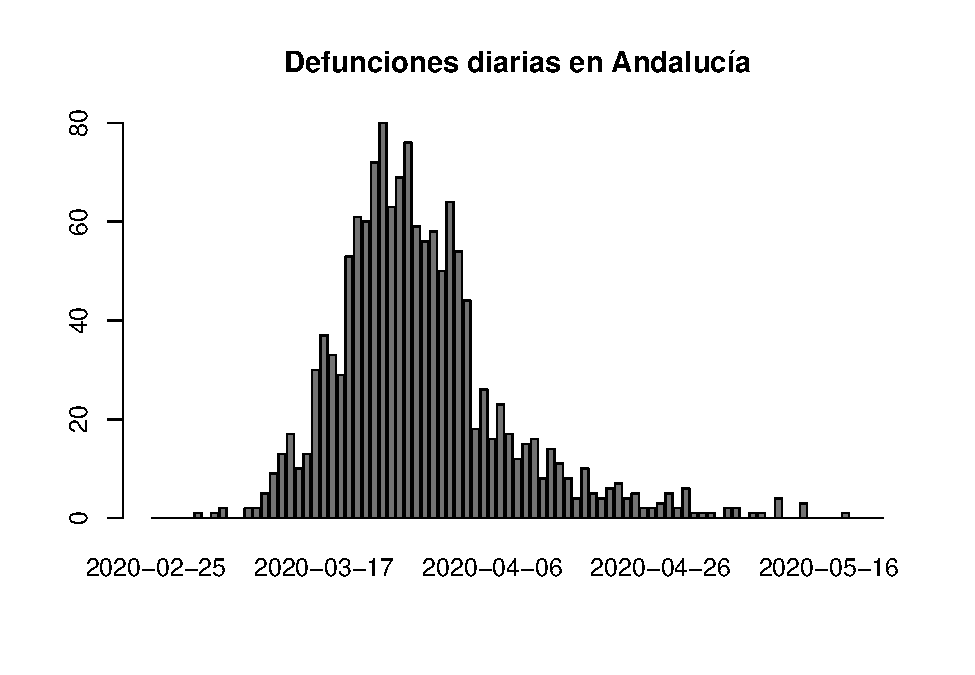
\includegraphics{bookdown-demo_files/figure-latex/unnamed-chunk-3-1.pdf}

\begin{Shaded}
\begin{Highlighting}[]
\KeywordTok{barplot}\NormalTok{(}\DataTypeTok{names.arg=}\NormalTok{aux}\OperatorTok{$}\StringTok{\textasciigrave{}}\DataTypeTok{Fecha declaración}\StringTok{\textasciigrave{}}\NormalTok{,aux}\OperatorTok{$}\NormalTok{Curados,}\DataTypeTok{main=}\StringTok{"Curaciones diarias en Andalucía"}\NormalTok{,}\DataTypeTok{col=}\StringTok{"limegreen"}\NormalTok{)}
\end{Highlighting}
\end{Shaded}

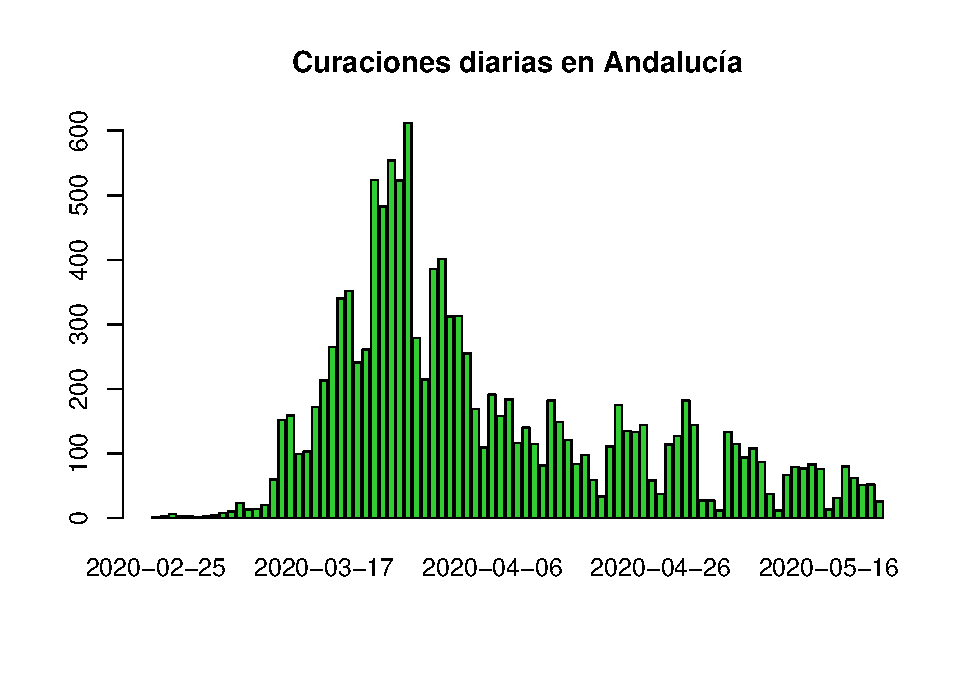
\includegraphics{bookdown-demo_files/figure-latex/unnamed-chunk-3-2.pdf}

\begin{Shaded}
\begin{Highlighting}[]
\KeywordTok{barplot}\NormalTok{(}\DataTypeTok{names.arg=}\NormalTok{aux}\OperatorTok{$}\StringTok{\textasciigrave{}}\DataTypeTok{Fecha declaración}\StringTok{\textasciigrave{}}\NormalTok{,aux}\OperatorTok{$}\NormalTok{Hospitalizados,}\DataTypeTok{main=}\StringTok{"Hospitalizaciones diarias en Andalucía"}\NormalTok{,}\DataTypeTok{col=}\StringTok{"mediumorchid4"}\NormalTok{)}
\end{Highlighting}
\end{Shaded}

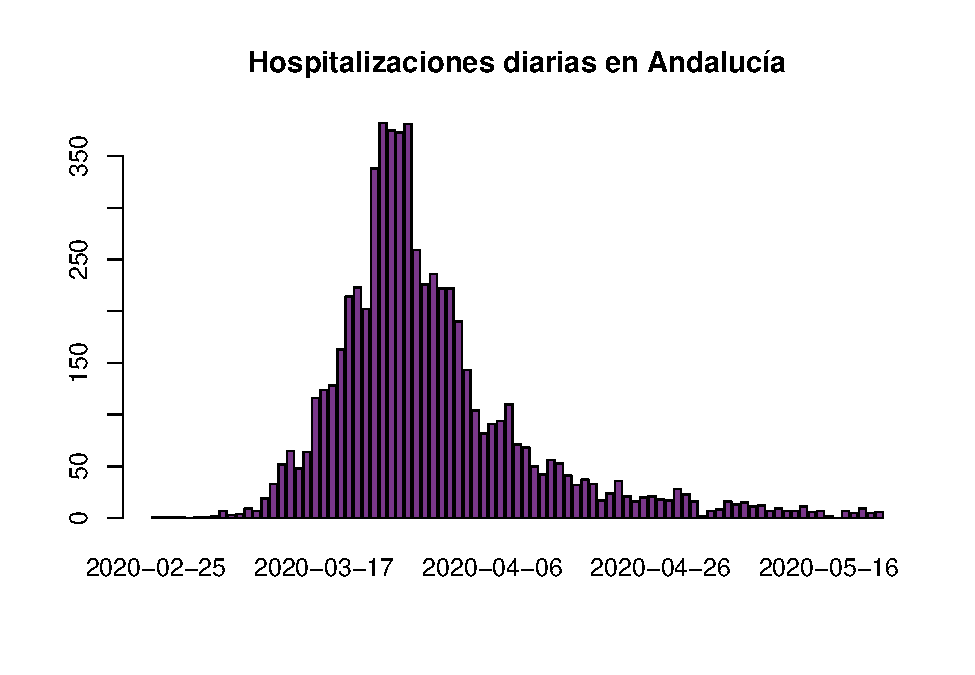
\includegraphics{bookdown-demo_files/figure-latex/unnamed-chunk-3-3.pdf}

\begin{Shaded}
\begin{Highlighting}[]
\KeywordTok{barplot}\NormalTok{(}\DataTypeTok{names.arg=}\NormalTok{aux}\OperatorTok{$}\StringTok{\textasciigrave{}}\DataTypeTok{Fecha declaración}\StringTok{\textasciigrave{}}\NormalTok{,aux}\OperatorTok{$}\NormalTok{UCI,}\DataTypeTok{main=}\StringTok{"Ingresos diarios en UCI en Andalucía"}\NormalTok{,}\DataTypeTok{col=}\StringTok{"tomato3"}\NormalTok{)}
\end{Highlighting}
\end{Shaded}

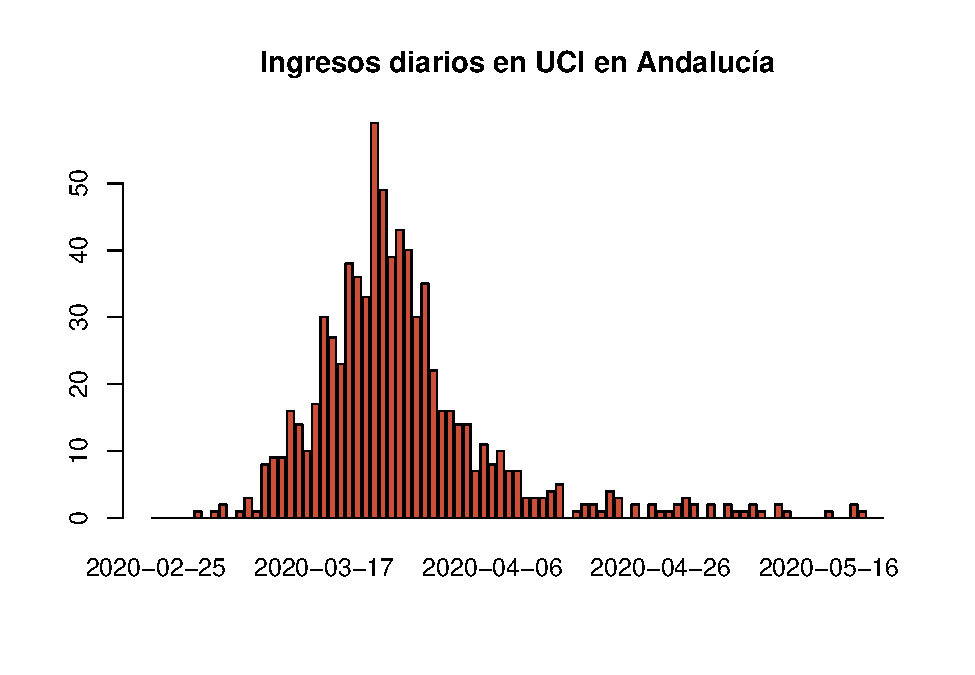
\includegraphics{bookdown-demo_files/figure-latex/unnamed-chunk-3-4.pdf}

\begin{Shaded}
\begin{Highlighting}[]
\KeywordTok{barplot}\NormalTok{(}\DataTypeTok{names.arg=}\NormalTok{aux}\OperatorTok{$}\StringTok{\textasciigrave{}}\DataTypeTok{Fecha declaración}\StringTok{\textasciigrave{}}\NormalTok{,aux}\OperatorTok{$}\StringTok{\textasciigrave{}}\DataTypeTok{Confirmados PCR}\StringTok{\textasciigrave{}}\NormalTok{,}\DataTypeTok{main=}\StringTok{"Positivos en test PCR en Andalucía"}\NormalTok{,}\DataTypeTok{col=}\StringTok{"orange2"}\NormalTok{)}
\end{Highlighting}
\end{Shaded}

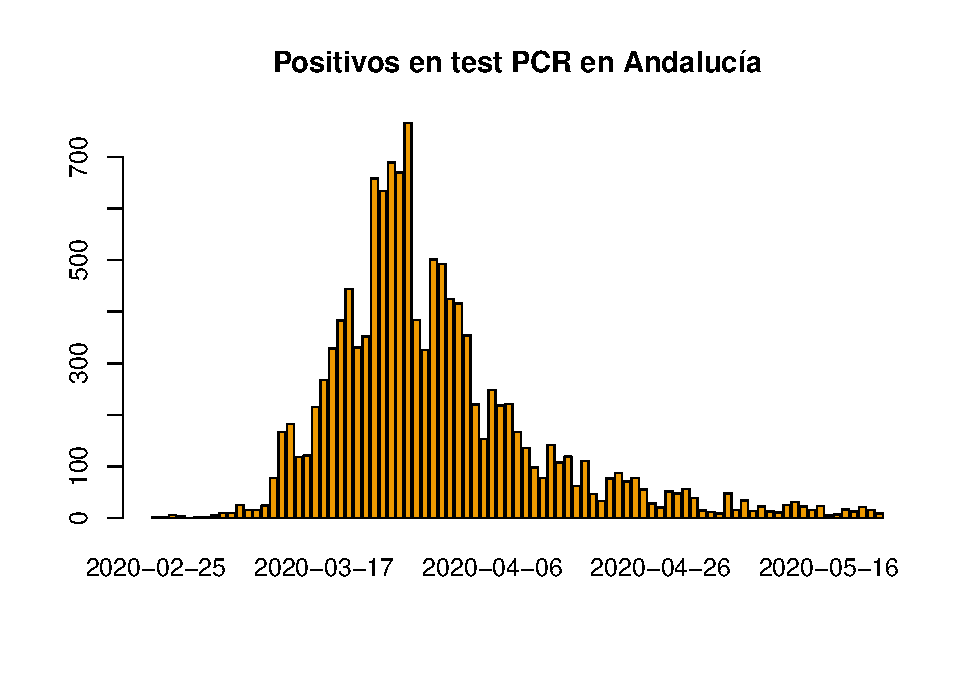
\includegraphics{bookdown-demo_files/figure-latex/unnamed-chunk-3-5.pdf}

\begin{Shaded}
\begin{Highlighting}[]
\KeywordTok{barplot}\NormalTok{(}\DataTypeTok{names.arg=}\NormalTok{aux}\OperatorTok{$}\StringTok{\textasciigrave{}}\DataTypeTok{Fecha declaración}\StringTok{\textasciigrave{}}\NormalTok{,aux}\OperatorTok{$}\StringTok{\textasciigrave{}}\DataTypeTok{Total confirmados (PCR+test)}\StringTok{\textasciigrave{}}\NormalTok{,}\DataTypeTok{ylim=}\KeywordTok{c}\NormalTok{(}\DecValTok{0}\NormalTok{,}\KeywordTok{max}\NormalTok{(aux}\OperatorTok{$}\StringTok{\textasciigrave{}}\DataTypeTok{Total confirmados (PCR+test)}\StringTok{\textasciigrave{}}\NormalTok{)),}\DataTypeTok{main=}\StringTok{"Confirmados diarios en Andalucía (PCR+test)"}\NormalTok{,}\DataTypeTok{col=}\StringTok{"orange4"}\NormalTok{)}
\end{Highlighting}
\end{Shaded}

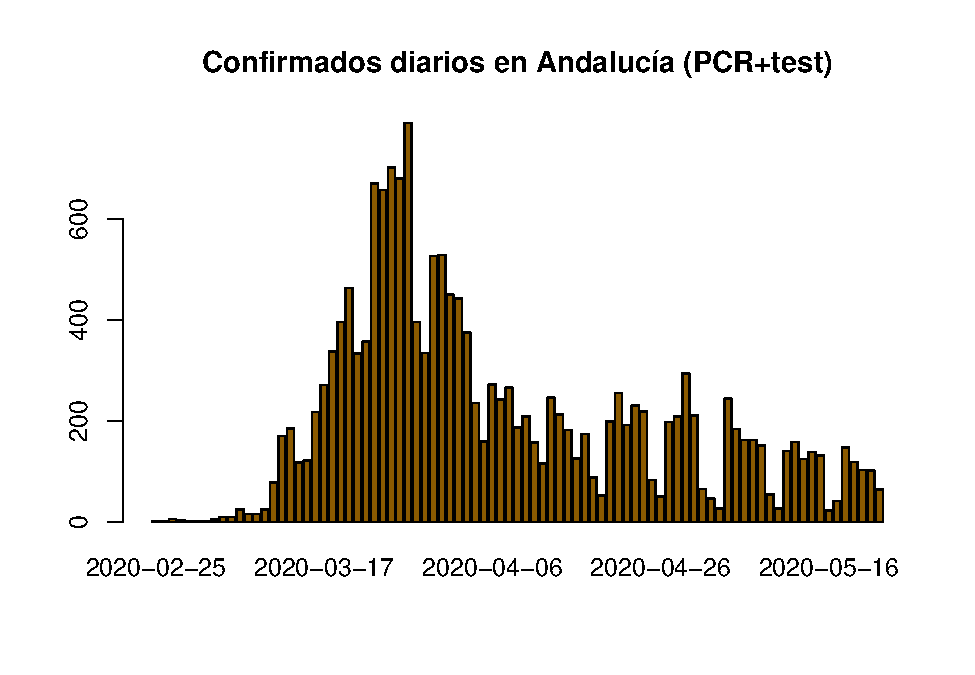
\includegraphics{bookdown-demo_files/figure-latex/unnamed-chunk-3-6.pdf}

\hypertarget{map-of-andalusia}{%
\section{Map of Andalusia}\label{map-of-andalusia}}

\begin{Shaded}
\begin{Highlighting}[]
\CommentTok{\# para manipular dataframes}
\KeywordTok{library}\NormalTok{(tidyverse)}
\CommentTok{\# para importar archivos shapefiles y excel}
\KeywordTok{library}\NormalTok{(rgdal)}
\KeywordTok{library}\NormalTok{(readxl)}
\CommentTok{\# Para transformar los archivos shapefiles }
\KeywordTok{library}\NormalTok{(broom)}
\KeywordTok{library}\NormalTok{(ggplot2)}
\KeywordTok{library}\NormalTok{(plotly)}
\CommentTok{\# Guardamos el archivo shapefile}
\NormalTok{shapefile\_provincias \textless{}{-}}\StringTok{ }\NormalTok{rgdal}\OperatorTok{::}\KeywordTok{readOGR}\NormalTok{(}\StringTok{"Provincias\_ETRS89\_30N/Provincias\_ETRS89\_30N.shp"}\NormalTok{)}
\end{Highlighting}
\end{Shaded}

\begin{verbatim}
## OGR data source with driver: ESRI Shapefile 
## Source: "C:\Users\Beatriz Huertas\Desktop\3º Ingeniería informática\2º cuatrimestre\Laboratorio de computación científica\Book covid analysis\Provincias_ETRS89_30N\Provincias_ETRS89_30N.shp", layer: "Provincias_ETRS89_30N"
## with 52 features
## It has 5 fields
\end{verbatim}

\begin{Shaded}
\begin{Highlighting}[]
\CommentTok{\# Para convertir el archivo shapefile en un dataframe utilizamos la función tidy()}
\NormalTok{data\_provincias \textless{}{-}}\StringTok{ }\KeywordTok{tidy}\NormalTok{(shapefile\_provincias)}
\NormalTok{nombres\_provincias \textless{}{-}}\StringTok{ }\KeywordTok{data.frame}\NormalTok{(shapefile\_provincias}\OperatorTok{$}\NormalTok{Texto)}
\NormalTok{nombres\_provincias}\OperatorTok{$}\NormalTok{id \textless{}{-}}\StringTok{ }\KeywordTok{as.character}\NormalTok{(}\KeywordTok{seq}\NormalTok{(}\DecValTok{0}\NormalTok{, }\KeywordTok{nrow}\NormalTok{(nombres\_provincias)}\OperatorTok{{-}}\DecValTok{1}\NormalTok{))}
\KeywordTok{head}\NormalTok{(nombres\_provincias)}
\end{Highlighting}
\end{Shaded}

\begin{verbatim}
##   shapefile_provincias.Texto id
## 1                     Ã\201lava  0
## 2                   Albacete  1
## 3                   Alicante  2
## 4                   Almería  3
## 5                     Ã\201vila  4
## 6                    Badajoz  5
\end{verbatim}

\begin{Shaded}
\begin{Highlighting}[]
\NormalTok{data\_provincias\_mapa \textless{}{-}}\StringTok{ }\KeywordTok{left\_join}\NormalTok{(data\_provincias, nombres\_provincias, }\DataTypeTok{by =} \StringTok{"id"}\NormalTok{)}
\NormalTok{reemplazos \textless{}{-}}\KeywordTok{cbind}\NormalTok{(data\_provincias,}\KeywordTok{gsub}\NormalTok{(}\StringTok{"Almer�a"}\NormalTok{,}\StringTok{"Almeria"}\NormalTok{, data\_provincias\_mapa}\OperatorTok{$}\NormalTok{shapefile\_provincias.Texto)                   )}
\KeywordTok{colnames}\NormalTok{(reemplazos)[}\DecValTok{8}\NormalTok{] \textless{}{-}}\StringTok{ "Provincias"}
\NormalTok{reemplazos}\OperatorTok{$}\NormalTok{Provincias \textless{}{-}}\StringTok{ }\KeywordTok{as.character}\NormalTok{(reemplazos}\OperatorTok{$}\NormalTok{Provincias)}
\NormalTok{reemplazos}\OperatorTok{$}\NormalTok{Provincias[}\DecValTok{2443}\OperatorTok{:}\DecValTok{3298}\NormalTok{] \textless{}{-}}\StringTok{ "Almeria"}
\NormalTok{reemplazos}\OperatorTok{$}\NormalTok{Provincias \textless{}{-}}\StringTok{ }\KeywordTok{as.factor}\NormalTok{(reemplazos}\OperatorTok{$}\NormalTok{Provincias)}
\NormalTok{provinciasandalucia \textless{}{-}}\StringTok{ }\KeywordTok{filter}\NormalTok{(reemplazos,reemplazos}\OperatorTok{$}\NormalTok{Provincias }\OperatorTok{\%in\%}\StringTok{ }\KeywordTok{c}\NormalTok{(}\StringTok{"Sevilla"}\NormalTok{,}\StringTok{"Huelva"}\NormalTok{,}\StringTok{"Córdoba"}\NormalTok{,}\StringTok{"Málaga"}\NormalTok{,}\StringTok{"Jaén"}\NormalTok{,}\StringTok{"Almeria"}\NormalTok{,}\StringTok{"Cádiz"}\NormalTok{,}\StringTok{"Granada"}\NormalTok{))}
\NormalTok{cs\_export \textless{}{-}}\StringTok{ }\KeywordTok{read\_excel}\NormalTok{(}\StringTok{"cs\_export.xls"}\NormalTok{) }\OperatorTok{\%\textgreater{}\%}\StringTok{ }\KeywordTok{print}\NormalTok{()}
\end{Highlighting}
\end{Shaded}

\begin{verbatim}
## # A tibble: 687 x 8
##    `Fecha declarac~ Territorio `Confirmados PC~ Hospitalizados   UCI Curados
##    <chr>            <chr>                 <dbl>          <dbl> <dbl>   <dbl>
##  1 22/05/2020       Andalucía                 9              6     0      26
##  2 22/05/2020       Almería                   1              2     0       4
##  3 22/05/2020       Córdoba                   0              0     0       1
##  4 22/05/2020       Granada                   0              1     0      11
##  5 22/05/2020       Huelva                    1              1     0       0
##  6 22/05/2020       Jaén                      5              2     0       1
##  7 22/05/2020       Málaga                    2              0     0       5
##  8 22/05/2020       Sevilla                   0              0     0       4
##  9 21/05/2020       Andalucía                16              5     0      52
## 10 21/05/2020       Almería                   0              0     0       4
## # ... with 677 more rows, and 2 more variables: Defunciones <dbl>, `Total
## #   confirmados (PCR+test)` <dbl>
\end{verbatim}

\begin{Shaded}
\begin{Highlighting}[]
\CommentTok{\# proceso los datos a utlizar}
\NormalTok{confirmados \textless{}{-}}\StringTok{ }
\StringTok{  }\NormalTok{cs\_export }\OperatorTok{\%\textgreater{}\%}\StringTok{ }
\StringTok{  }\KeywordTok{group\_by}\NormalTok{(Territorio, }\StringTok{\textasciigrave{}}\DataTypeTok{Fecha declaración}\StringTok{\textasciigrave{}}\NormalTok{)}\OperatorTok{\%\textgreater{}\%}\StringTok{ }
\StringTok{  }\KeywordTok{print}\NormalTok{()}
\end{Highlighting}
\end{Shaded}

\begin{verbatim}
## # A tibble: 687 x 8
## # Groups:   Territorio, Fecha declaración [686]
##    `Fecha declarac~ Territorio `Confirmados PC~ Hospitalizados   UCI Curados
##    <chr>            <chr>                 <dbl>          <dbl> <dbl>   <dbl>
##  1 22/05/2020       Andalucía                 9              6     0      26
##  2 22/05/2020       Almería                   1              2     0       4
##  3 22/05/2020       Córdoba                   0              0     0       1
##  4 22/05/2020       Granada                   0              1     0      11
##  5 22/05/2020       Huelva                    1              1     0       0
##  6 22/05/2020       Jaén                      5              2     0       1
##  7 22/05/2020       Málaga                    2              0     0       5
##  8 22/05/2020       Sevilla                   0              0     0       4
##  9 21/05/2020       Andalucía                16              5     0      52
## 10 21/05/2020       Almería                   0              0     0       4
## # ... with 677 more rows, and 2 more variables: Defunciones <dbl>, `Total
## #   confirmados (PCR+test)` <dbl>
\end{verbatim}

\begin{Shaded}
\begin{Highlighting}[]
\NormalTok{almeria \textless{}{-}}\StringTok{ }\NormalTok{confirmados }\OperatorTok{\%\textgreater{}\%}\StringTok{ }\KeywordTok{filter}\NormalTok{(Territorio}\OperatorTok{==}\StringTok{"Almería"}\NormalTok{)}
\NormalTok{almeriaacum \textless{}{-}}\StringTok{ }\KeywordTok{colSums}\NormalTok{(almeria[}\DecValTok{3}\OperatorTok{:}\DecValTok{8}\NormalTok{])}
\NormalTok{cadiz \textless{}{-}}\StringTok{ }\NormalTok{confirmados }\OperatorTok{\%\textgreater{}\%}\StringTok{ }\KeywordTok{filter}\NormalTok{(Territorio}\OperatorTok{==}\StringTok{"Cádiz"}\NormalTok{)}
\NormalTok{cadizacum \textless{}{-}}\StringTok{ }\KeywordTok{colSums}\NormalTok{(cadiz[}\DecValTok{3}\OperatorTok{:}\DecValTok{8}\NormalTok{])}
\NormalTok{cordoba \textless{}{-}}\StringTok{ }\NormalTok{confirmados }\OperatorTok{\%\textgreater{}\%}\StringTok{ }\KeywordTok{filter}\NormalTok{(Territorio}\OperatorTok{==}\StringTok{"Córdoba"}\NormalTok{)}
\NormalTok{cordobaacum \textless{}{-}}\StringTok{ }\KeywordTok{colSums}\NormalTok{(cordoba[}\DecValTok{3}\OperatorTok{:}\DecValTok{8}\NormalTok{])}
\NormalTok{granada \textless{}{-}}\StringTok{ }\NormalTok{confirmados }\OperatorTok{\%\textgreater{}\%}\StringTok{ }\KeywordTok{filter}\NormalTok{(Territorio}\OperatorTok{==}\StringTok{"Granada"}\NormalTok{)}
\NormalTok{granadaacum \textless{}{-}}\StringTok{ }\KeywordTok{colSums}\NormalTok{(granada[}\DecValTok{3}\OperatorTok{:}\DecValTok{8}\NormalTok{])}
\NormalTok{huelva \textless{}{-}}\StringTok{ }\NormalTok{confirmados }\OperatorTok{\%\textgreater{}\%}\StringTok{ }\KeywordTok{filter}\NormalTok{(Territorio}\OperatorTok{==}\StringTok{"Huelva"}\NormalTok{)}
\NormalTok{huelvaacum \textless{}{-}}\StringTok{ }\KeywordTok{colSums}\NormalTok{(huelva[}\DecValTok{3}\OperatorTok{:}\DecValTok{8}\NormalTok{])}
\NormalTok{jaen \textless{}{-}}\StringTok{ }\NormalTok{confirmados }\OperatorTok{\%\textgreater{}\%}\StringTok{ }\KeywordTok{filter}\NormalTok{(Territorio}\OperatorTok{==}\StringTok{"Jaén"}\NormalTok{)}
\NormalTok{jaenacum \textless{}{-}}\StringTok{ }\KeywordTok{colSums}\NormalTok{(jaen[}\DecValTok{3}\OperatorTok{:}\DecValTok{8}\NormalTok{])}
\NormalTok{malaga \textless{}{-}}\StringTok{ }\NormalTok{confirmados }\OperatorTok{\%\textgreater{}\%}\StringTok{ }\KeywordTok{filter}\NormalTok{(Territorio}\OperatorTok{==}\StringTok{"Málaga"}\NormalTok{)}
\NormalTok{malagaacum \textless{}{-}}\StringTok{ }\KeywordTok{colSums}\NormalTok{(malaga[}\DecValTok{3}\OperatorTok{:}\DecValTok{8}\NormalTok{])}
\NormalTok{sevilla \textless{}{-}}\StringTok{ }\NormalTok{confirmados }\OperatorTok{\%\textgreater{}\%}\StringTok{ }\KeywordTok{filter}\NormalTok{(Territorio}\OperatorTok{==}\StringTok{"Sevilla"}\NormalTok{)}
\NormalTok{sevillaacum \textless{}{-}}\StringTok{ }\KeywordTok{colSums}\NormalTok{(sevilla[}\DecValTok{3}\OperatorTok{:}\DecValTok{8}\NormalTok{])}
\NormalTok{dfaux \textless{}{-}}\StringTok{ }\KeywordTok{data.frame}\NormalTok{(}\StringTok{"Provincia"}\NormalTok{=}\KeywordTok{c}\NormalTok{(}\StringTok{"Sevilla"}\NormalTok{,}\StringTok{"Málaga"}\NormalTok{,}\StringTok{"Jaén"}\NormalTok{,}\StringTok{"Huelva"}\NormalTok{,}\StringTok{"Granada"}\NormalTok{,}\StringTok{"Córdoba"}\NormalTok{,}\StringTok{"Cádiz"}\NormalTok{,}\StringTok{"AlmerÃ�a"}\NormalTok{),}\StringTok{"Confirmados"}\NormalTok{=}\KeywordTok{c}\NormalTok{(sevillaacum[}\DecValTok{6}\NormalTok{],malagaacum[}\DecValTok{6}\NormalTok{],jaenacum[}\DecValTok{6}\NormalTok{],huelvaacum[}\DecValTok{6}\NormalTok{],granadaacum[}\DecValTok{6}\NormalTok{],cordobaacum[}\DecValTok{6}\NormalTok{],cadizacum[}\DecValTok{6}\NormalTok{],almeriaacum[}\DecValTok{6}\NormalTok{]),}\StringTok{"Hospitalizados"}\NormalTok{=}\KeywordTok{c}\NormalTok{(sevillaacum[}\DecValTok{2}\NormalTok{],malagaacum[}\DecValTok{2}\NormalTok{],jaenacum[}\DecValTok{2}\NormalTok{],huelvaacum[}\DecValTok{2}\NormalTok{],granadaacum[}\DecValTok{2}\NormalTok{],cordobaacum[}\DecValTok{2}\NormalTok{],cadizacum[}\DecValTok{2}\NormalTok{],almeriaacum[}\DecValTok{2}\NormalTok{]),}\StringTok{"Curados"}\NormalTok{=}\KeywordTok{c}\NormalTok{(sevillaacum[}\DecValTok{4}\NormalTok{],malagaacum[}\DecValTok{4}\NormalTok{],jaenacum[}\DecValTok{4}\NormalTok{],huelvaacum[}\DecValTok{4}\NormalTok{],granadaacum[}\DecValTok{4}\NormalTok{],cordobaacum[}\DecValTok{4}\NormalTok{],cadizacum[}\DecValTok{4}\NormalTok{],almeriaacum[}\DecValTok{4}\NormalTok{]),}\StringTok{"Defunciones"}\NormalTok{=}\KeywordTok{c}\NormalTok{(sevillaacum[}\DecValTok{5}\NormalTok{],malagaacum[}\DecValTok{5}\NormalTok{],jaenacum[}\DecValTok{5}\NormalTok{],huelvaacum[}\DecValTok{5}\NormalTok{],granadaacum[}\DecValTok{5}\NormalTok{],cordobaacum[}\DecValTok{5}\NormalTok{],cadizacum[}\DecValTok{5}\NormalTok{],almeriaacum[}\DecValTok{5}\NormalTok{]))}
\NormalTok{dfaux}\OperatorTok{$}\NormalTok{id \textless{}{-}}\StringTok{ }\KeywordTok{as.character}\NormalTok{(}\KeywordTok{c}\NormalTok{(}\DecValTok{40}\NormalTok{,}\DecValTok{28}\NormalTok{,}\DecValTok{22}\NormalTok{,}\DecValTok{20}\NormalTok{,}\DecValTok{17}\NormalTok{,}\DecValTok{13}\NormalTok{,}\DecValTok{10}\NormalTok{,}\DecValTok{3}\NormalTok{))}
\NormalTok{confirmadosmapa \textless{}{-}}\StringTok{ }\NormalTok{provinciasandalucia }\OperatorTok{\%\textgreater{}\%}\StringTok{ }
\StringTok{  }\KeywordTok{left\_join}\NormalTok{(dfaux, }\DataTypeTok{by=} \StringTok{"id"}\NormalTok{)}
\NormalTok{mapa \textless{}{-}}\StringTok{ }\NormalTok{confirmadosmapa }\OperatorTok{\%\textgreater{}\%}
\StringTok{  }\KeywordTok{ggplot}\NormalTok{(}\KeywordTok{aes}\NormalTok{(}\DataTypeTok{x=}\NormalTok{long, }\DataTypeTok{y=}\NormalTok{ lat, }\DataTypeTok{group =}\NormalTok{ group)) }\OperatorTok{+}
\StringTok{  }\KeywordTok{geom\_polygon}\NormalTok{(}\KeywordTok{aes}\NormalTok{(}\DataTypeTok{fill=}\NormalTok{Confirmados), }\DataTypeTok{color=} \StringTok{"white"}\NormalTok{, }\DataTypeTok{size =} \FloatTok{0.2}\NormalTok{) }\OperatorTok{+}
\StringTok{  }\KeywordTok{labs}\NormalTok{( }\DataTypeTok{title =} \StringTok{"Tasa de Contagios por Provincia"}\NormalTok{,}
        \DataTypeTok{fill =} \StringTok{""}\NormalTok{) }\OperatorTok{+}
\StringTok{  }\KeywordTok{theme\_minimal}\NormalTok{() }\OperatorTok{+}
\StringTok{  }\KeywordTok{theme}\NormalTok{(}
    \DataTypeTok{axis.line =} \KeywordTok{element\_blank}\NormalTok{(),}
    \DataTypeTok{axis.text =} \KeywordTok{element\_blank}\NormalTok{(),}
    \DataTypeTok{axis.title =} \KeywordTok{element\_blank}\NormalTok{(),}
    \DataTypeTok{axis.ticks =} \KeywordTok{element\_blank}\NormalTok{(),}
    \DataTypeTok{plot.background =} \KeywordTok{element\_rect}\NormalTok{(}\DataTypeTok{fill =} \StringTok{"snow"}\NormalTok{, }\DataTypeTok{color =} \OtherTok{NA}\NormalTok{),}
    \DataTypeTok{panel.background =} \KeywordTok{element\_rect}\NormalTok{(}\DataTypeTok{fill=} \StringTok{"snow"}\NormalTok{, }\DataTypeTok{color =} \OtherTok{NA}\NormalTok{),}
    \DataTypeTok{plot.title =} \KeywordTok{element\_text}\NormalTok{(}\DataTypeTok{size =} \DecValTok{16}\NormalTok{, }\DataTypeTok{hjust =} \DecValTok{0}\NormalTok{),}
    \DataTypeTok{plot.subtitle =} \KeywordTok{element\_text}\NormalTok{(}\DataTypeTok{size =} \DecValTok{12}\NormalTok{, }\DataTypeTok{hjust =} \DecValTok{0}\NormalTok{),}
    \DataTypeTok{plot.caption =} \KeywordTok{element\_text}\NormalTok{(}\DataTypeTok{size =} \DecValTok{8}\NormalTok{, }\DataTypeTok{hjust =} \DecValTok{1}\NormalTok{),}
    \DataTypeTok{legend.title =} \KeywordTok{element\_text}\NormalTok{(}\DataTypeTok{color =} \StringTok{"grey40"}\NormalTok{, }\DataTypeTok{size =} \DecValTok{8}\NormalTok{),}
    \DataTypeTok{legend.text =} \KeywordTok{element\_text}\NormalTok{(}\DataTypeTok{color =} \StringTok{"grey40"}\NormalTok{, }\DataTypeTok{size =} \DecValTok{7}\NormalTok{, }\DataTypeTok{hjust =} \DecValTok{0}\NormalTok{),}
    \DataTypeTok{legend.position =} \KeywordTok{c}\NormalTok{(}\FloatTok{0.93}\NormalTok{, }\FloatTok{0.3}\NormalTok{),}
    \DataTypeTok{plot.margin =} \KeywordTok{unit}\NormalTok{(}\KeywordTok{c}\NormalTok{(}\FloatTok{0.5}\NormalTok{,}\DecValTok{2}\NormalTok{,}\FloatTok{0.5}\NormalTok{,}\DecValTok{1}\NormalTok{), }\StringTok{"cm"}\NormalTok{)) }\OperatorTok{+}
\StringTok{  }\KeywordTok{scale\_fill\_gradient}\NormalTok{(}\DataTypeTok{low =} \StringTok{"yellow"}\NormalTok{, }\DataTypeTok{high =} \StringTok{"red"}\NormalTok{)}
\KeywordTok{ggplotly}\NormalTok{(mapa) }\OperatorTok{\%\textgreater{}\%}\StringTok{  }
\StringTok{  }\KeywordTok{layout}\NormalTok{(}\DataTypeTok{title =} \StringTok{\textquotesingle{}Tasa de Contagios por Provincia\textquotesingle{}}\NormalTok{)}
\end{Highlighting}
\end{Shaded}

\hypertarget{htmlwidget-7aeae24ee6aa7dccd339}{}

\begin{Shaded}
\begin{Highlighting}[]
\CommentTok{\#\# Hospitalizados}
\NormalTok{mapa \textless{}{-}}\StringTok{ }\NormalTok{confirmadosmapa }\OperatorTok{\%\textgreater{}\%}
\StringTok{  }\KeywordTok{ggplot}\NormalTok{(}\KeywordTok{aes}\NormalTok{(}\DataTypeTok{x=}\NormalTok{long, }\DataTypeTok{y=}\NormalTok{ lat, }\DataTypeTok{group =}\NormalTok{ group)) }\OperatorTok{+}
\StringTok{  }\KeywordTok{geom\_polygon}\NormalTok{(}\KeywordTok{aes}\NormalTok{(}\DataTypeTok{fill=}\NormalTok{Hospitalizados), }\DataTypeTok{color=} \StringTok{"white"}\NormalTok{, }\DataTypeTok{size =} \FloatTok{0.2}\NormalTok{) }\OperatorTok{+}
\StringTok{  }\KeywordTok{labs}\NormalTok{( }\DataTypeTok{title =} \StringTok{"Tasa de Hospitalizados por Provincia"}\NormalTok{,}
        \DataTypeTok{fill =} \StringTok{""}\NormalTok{) }\OperatorTok{+}
\StringTok{  }\KeywordTok{theme\_minimal}\NormalTok{() }\OperatorTok{+}
\StringTok{  }\KeywordTok{theme}\NormalTok{(}
    \DataTypeTok{axis.line =} \KeywordTok{element\_blank}\NormalTok{(),}
    \DataTypeTok{axis.text =} \KeywordTok{element\_blank}\NormalTok{(),}
    \DataTypeTok{axis.title =} \KeywordTok{element\_blank}\NormalTok{(),}
    \DataTypeTok{axis.ticks =} \KeywordTok{element\_blank}\NormalTok{(),}
    \DataTypeTok{plot.background =} \KeywordTok{element\_rect}\NormalTok{(}\DataTypeTok{fill =} \StringTok{"snow"}\NormalTok{, }\DataTypeTok{color =} \OtherTok{NA}\NormalTok{),}
    \DataTypeTok{panel.background =} \KeywordTok{element\_rect}\NormalTok{(}\DataTypeTok{fill=} \StringTok{"snow"}\NormalTok{, }\DataTypeTok{color =} \OtherTok{NA}\NormalTok{),}
    \DataTypeTok{plot.title =} \KeywordTok{element\_text}\NormalTok{(}\DataTypeTok{size =} \DecValTok{16}\NormalTok{, }\DataTypeTok{hjust =} \DecValTok{0}\NormalTok{),}
    \DataTypeTok{plot.subtitle =} \KeywordTok{element\_text}\NormalTok{(}\DataTypeTok{size =} \DecValTok{12}\NormalTok{, }\DataTypeTok{hjust =} \DecValTok{0}\NormalTok{),}
    \DataTypeTok{plot.caption =} \KeywordTok{element\_text}\NormalTok{(}\DataTypeTok{size =} \DecValTok{8}\NormalTok{, }\DataTypeTok{hjust =} \DecValTok{1}\NormalTok{),}
    \DataTypeTok{legend.title =} \KeywordTok{element\_text}\NormalTok{(}\DataTypeTok{color =} \StringTok{"grey40"}\NormalTok{, }\DataTypeTok{size =} \DecValTok{8}\NormalTok{),}
    \DataTypeTok{legend.text =} \KeywordTok{element\_text}\NormalTok{(}\DataTypeTok{color =} \StringTok{"grey40"}\NormalTok{, }\DataTypeTok{size =} \DecValTok{7}\NormalTok{, }\DataTypeTok{hjust =} \DecValTok{0}\NormalTok{),}
    \DataTypeTok{legend.position =} \KeywordTok{c}\NormalTok{(}\FloatTok{0.93}\NormalTok{, }\FloatTok{0.3}\NormalTok{),}
    \DataTypeTok{plot.margin =} \KeywordTok{unit}\NormalTok{(}\KeywordTok{c}\NormalTok{(}\FloatTok{0.5}\NormalTok{,}\DecValTok{2}\NormalTok{,}\FloatTok{0.5}\NormalTok{,}\DecValTok{1}\NormalTok{), }\StringTok{"cm"}\NormalTok{)) }\OperatorTok{+}
\StringTok{  }\KeywordTok{scale\_fill\_gradient}\NormalTok{(}\DataTypeTok{low =} \StringTok{"green"}\NormalTok{, }\DataTypeTok{high =} \StringTok{"red"}\NormalTok{)}
\KeywordTok{ggplotly}\NormalTok{(mapa) }\OperatorTok{\%\textgreater{}\%}\StringTok{  }
\StringTok{  }\KeywordTok{layout}\NormalTok{(}\DataTypeTok{title =} \StringTok{\textquotesingle{}Tasa de Hospitalizados por Provincia\textquotesingle{}}\NormalTok{)}
\end{Highlighting}
\end{Shaded}

\hypertarget{htmlwidget-1908f753aaf894b37f1e}{}

\begin{Shaded}
\begin{Highlighting}[]
\CommentTok{\#\# Curados}
\NormalTok{mapa \textless{}{-}}\StringTok{ }\NormalTok{confirmadosmapa }\OperatorTok{\%\textgreater{}\%}
\StringTok{  }\KeywordTok{ggplot}\NormalTok{(}\KeywordTok{aes}\NormalTok{(}\DataTypeTok{x=}\NormalTok{long, }\DataTypeTok{y=}\NormalTok{ lat, }\DataTypeTok{group =}\NormalTok{ group)) }\OperatorTok{+}
\StringTok{  }\KeywordTok{geom\_polygon}\NormalTok{(}\KeywordTok{aes}\NormalTok{(}\DataTypeTok{fill=}\NormalTok{Curados), }\DataTypeTok{color=} \StringTok{"white"}\NormalTok{, }\DataTypeTok{size =} \FloatTok{0.2}\NormalTok{) }\OperatorTok{+}
\StringTok{  }\KeywordTok{labs}\NormalTok{( }\DataTypeTok{title =} \StringTok{"Tasa de Curados por Provincia"}\NormalTok{,}
        \DataTypeTok{fill =} \StringTok{""}\NormalTok{) }\OperatorTok{+}
\StringTok{  }\KeywordTok{theme\_minimal}\NormalTok{() }\OperatorTok{+}
\StringTok{  }\KeywordTok{theme}\NormalTok{(}
    \DataTypeTok{axis.line =} \KeywordTok{element\_blank}\NormalTok{(),}
    \DataTypeTok{axis.text =} \KeywordTok{element\_blank}\NormalTok{(),}
    \DataTypeTok{axis.title =} \KeywordTok{element\_blank}\NormalTok{(),}
    \DataTypeTok{axis.ticks =} \KeywordTok{element\_blank}\NormalTok{(),}
    \DataTypeTok{plot.background =} \KeywordTok{element\_rect}\NormalTok{(}\DataTypeTok{fill =} \StringTok{"snow"}\NormalTok{, }\DataTypeTok{color =} \OtherTok{NA}\NormalTok{),}
    \DataTypeTok{panel.background =} \KeywordTok{element\_rect}\NormalTok{(}\DataTypeTok{fill=} \StringTok{"snow"}\NormalTok{, }\DataTypeTok{color =} \OtherTok{NA}\NormalTok{),}
    \DataTypeTok{plot.title =} \KeywordTok{element\_text}\NormalTok{(}\DataTypeTok{size =} \DecValTok{16}\NormalTok{, }\DataTypeTok{hjust =} \DecValTok{0}\NormalTok{),}
    \DataTypeTok{plot.subtitle =} \KeywordTok{element\_text}\NormalTok{(}\DataTypeTok{size =} \DecValTok{12}\NormalTok{, }\DataTypeTok{hjust =} \DecValTok{0}\NormalTok{),}
    \DataTypeTok{plot.caption =} \KeywordTok{element\_text}\NormalTok{(}\DataTypeTok{size =} \DecValTok{8}\NormalTok{, }\DataTypeTok{hjust =} \DecValTok{1}\NormalTok{),}
    \DataTypeTok{legend.title =} \KeywordTok{element\_text}\NormalTok{(}\DataTypeTok{color =} \StringTok{"grey40"}\NormalTok{, }\DataTypeTok{size =} \DecValTok{8}\NormalTok{),}
    \DataTypeTok{legend.text =} \KeywordTok{element\_text}\NormalTok{(}\DataTypeTok{color =} \StringTok{"grey40"}\NormalTok{, }\DataTypeTok{size =} \DecValTok{7}\NormalTok{, }\DataTypeTok{hjust =} \DecValTok{0}\NormalTok{),}
    \DataTypeTok{legend.position =} \KeywordTok{c}\NormalTok{(}\FloatTok{0.93}\NormalTok{, }\FloatTok{0.3}\NormalTok{),}
    \DataTypeTok{plot.margin =} \KeywordTok{unit}\NormalTok{(}\KeywordTok{c}\NormalTok{(}\FloatTok{0.5}\NormalTok{,}\DecValTok{2}\NormalTok{,}\FloatTok{0.5}\NormalTok{,}\DecValTok{1}\NormalTok{), }\StringTok{"cm"}\NormalTok{)) }\OperatorTok{+}
\StringTok{  }\KeywordTok{scale\_fill\_gradient}\NormalTok{(}\DataTypeTok{low =}\StringTok{"aquamarine"}\NormalTok{, }\DataTypeTok{high =} \StringTok{"darkblue"}\NormalTok{)}
\KeywordTok{ggplotly}\NormalTok{(mapa) }\OperatorTok{\%\textgreater{}\%}\StringTok{  }
\StringTok{  }\KeywordTok{layout}\NormalTok{(}\DataTypeTok{title =} \StringTok{\textquotesingle{}Tasa de Curados por Provincia\textquotesingle{}}\NormalTok{)}
\end{Highlighting}
\end{Shaded}

\hypertarget{htmlwidget-fa43c3e4e6439b0c5aa5}{}

\begin{Shaded}
\begin{Highlighting}[]
\CommentTok{\#\# Defunciones}
\NormalTok{mapa \textless{}{-}}\StringTok{ }\NormalTok{confirmadosmapa }\OperatorTok{\%\textgreater{}\%}
\StringTok{  }\KeywordTok{ggplot}\NormalTok{(}\KeywordTok{aes}\NormalTok{(}\DataTypeTok{x=}\NormalTok{long, }\DataTypeTok{y=}\NormalTok{ lat, }\DataTypeTok{group =}\NormalTok{ group)) }\OperatorTok{+}
\StringTok{  }\KeywordTok{geom\_polygon}\NormalTok{(}\KeywordTok{aes}\NormalTok{(}\DataTypeTok{fill=}\NormalTok{Defunciones), }\DataTypeTok{color=} \StringTok{"white"}\NormalTok{, }\DataTypeTok{size =} \FloatTok{0.2}\NormalTok{) }\OperatorTok{+}
\StringTok{  }\KeywordTok{labs}\NormalTok{( }\DataTypeTok{title =} \StringTok{"Tasa de Defunciones por Provincia"}\NormalTok{,}
        \DataTypeTok{fill =} \StringTok{""}\NormalTok{) }\OperatorTok{+}
\StringTok{  }\KeywordTok{theme\_minimal}\NormalTok{() }\OperatorTok{+}
\StringTok{  }\KeywordTok{theme}\NormalTok{(}
    \DataTypeTok{axis.line =} \KeywordTok{element\_blank}\NormalTok{(),}
    \DataTypeTok{axis.text =} \KeywordTok{element\_blank}\NormalTok{(),}
    \DataTypeTok{axis.title =} \KeywordTok{element\_blank}\NormalTok{(),}
    \DataTypeTok{axis.ticks =} \KeywordTok{element\_blank}\NormalTok{(),}
    \DataTypeTok{plot.background =} \KeywordTok{element\_rect}\NormalTok{(}\DataTypeTok{fill =} \StringTok{"snow"}\NormalTok{, }\DataTypeTok{color =} \OtherTok{NA}\NormalTok{),}
    \DataTypeTok{panel.background =} \KeywordTok{element\_rect}\NormalTok{(}\DataTypeTok{fill=} \StringTok{"snow"}\NormalTok{, }\DataTypeTok{color =} \OtherTok{NA}\NormalTok{),}
    \DataTypeTok{plot.title =} \KeywordTok{element\_text}\NormalTok{(}\DataTypeTok{size =} \DecValTok{16}\NormalTok{, }\DataTypeTok{hjust =} \DecValTok{0}\NormalTok{),}
    \DataTypeTok{plot.subtitle =} \KeywordTok{element\_text}\NormalTok{(}\DataTypeTok{size =} \DecValTok{12}\NormalTok{, }\DataTypeTok{hjust =} \DecValTok{0}\NormalTok{),}
    \DataTypeTok{plot.caption =} \KeywordTok{element\_text}\NormalTok{(}\DataTypeTok{size =} \DecValTok{8}\NormalTok{, }\DataTypeTok{hjust =} \DecValTok{1}\NormalTok{),}
    \DataTypeTok{legend.title =} \KeywordTok{element\_text}\NormalTok{(}\DataTypeTok{color =} \StringTok{"grey40"}\NormalTok{, }\DataTypeTok{size =} \DecValTok{8}\NormalTok{),}
    \DataTypeTok{legend.text =} \KeywordTok{element\_text}\NormalTok{(}\DataTypeTok{color =} \StringTok{"grey40"}\NormalTok{, }\DataTypeTok{size =} \DecValTok{7}\NormalTok{, }\DataTypeTok{hjust =} \DecValTok{0}\NormalTok{),}
    \DataTypeTok{legend.position =} \KeywordTok{c}\NormalTok{(}\FloatTok{0.93}\NormalTok{, }\FloatTok{0.3}\NormalTok{),}
    \DataTypeTok{plot.margin =} \KeywordTok{unit}\NormalTok{(}\KeywordTok{c}\NormalTok{(}\FloatTok{0.5}\NormalTok{,}\DecValTok{2}\NormalTok{,}\FloatTok{0.5}\NormalTok{,}\DecValTok{1}\NormalTok{), }\StringTok{"cm"}\NormalTok{)) }\OperatorTok{+}
\StringTok{  }\KeywordTok{scale\_fill\_gradient}\NormalTok{(}\DataTypeTok{low =}\StringTok{"gray46"}\NormalTok{, }\DataTypeTok{high =} \StringTok{"gray8"}\NormalTok{)}
\KeywordTok{ggplotly}\NormalTok{(mapa) }\OperatorTok{\%\textgreater{}\%}\StringTok{  }
\StringTok{  }\KeywordTok{layout}\NormalTok{(}\DataTypeTok{title =} \StringTok{\textquotesingle{}Tasa de Defunciones por Provincia\textquotesingle{}}\NormalTok{)}
\end{Highlighting}
\end{Shaded}

\hypertarget{htmlwidget-a732c932f79a7ce8c7b1}{}

\hypertarget{association-rules}{%
\chapter{Association Rules}\label{association-rules}}

\begin{Shaded}
\begin{Highlighting}[]
\KeywordTok{library}\NormalTok{(readxl)}
\KeywordTok{library}\NormalTok{(dplyr)}
\KeywordTok{library}\NormalTok{(arules)}
\KeywordTok{library}\NormalTok{(arulesViz)}
\NormalTok{datos \textless{}{-}}\StringTok{ }\KeywordTok{read\_excel}\NormalTok{(}\StringTok{"cs\_export.xls"}\NormalTok{)}
\CommentTok{\#View(head(datos))}
\NormalTok{datos \textless{}{-}}\StringTok{ }\KeywordTok{na.omit}\NormalTok{(datos)}
\end{Highlighting}
\end{Shaded}

We split the data of each province from those of Andalusia

\begin{Shaded}
\begin{Highlighting}[]
\NormalTok{datos}\OperatorTok{$}\StringTok{\textasciigrave{}}\DataTypeTok{Fecha declaración}\StringTok{\textasciigrave{}}\NormalTok{ \textless{}{-}}\StringTok{ }\KeywordTok{as.Date}\NormalTok{(datos}\OperatorTok{$}\StringTok{\textasciigrave{}}\DataTypeTok{Fecha declaración}\StringTok{\textasciigrave{}}\NormalTok{, }\StringTok{"\%d/\%m/\%Y"}\NormalTok{)}
\NormalTok{datos}\OperatorTok{$}\NormalTok{Territorio \textless{}{-}}\StringTok{ }\KeywordTok{as.factor}\NormalTok{(datos}\OperatorTok{$}\NormalTok{Territorio)}
\NormalTok{filasandalucia \textless{}{-}}\StringTok{ }\KeywordTok{filter}\NormalTok{(datos, Territorio}\OperatorTok{==}\StringTok{"Andalucía"}\NormalTok{ )}
\NormalTok{provincias \textless{}{-}}\StringTok{ }\KeywordTok{setdiff}\NormalTok{(datos,filasandalucia)}
\KeywordTok{nrow}\NormalTok{(provincias)}
\end{Highlighting}
\end{Shaded}

\begin{verbatim}
## [1] 687
\end{verbatim}

\begin{Shaded}
\begin{Highlighting}[]
\KeywordTok{nrow}\NormalTok{(filasandalucia)}
\end{Highlighting}
\end{Shaded}

\begin{verbatim}
## [1] 87
\end{verbatim}

When working with numerical data the first step we have to carry out is to discretize them. The ICU and Death columns are very skewed so we use a different method.

\begin{Shaded}
\begin{Highlighting}[]
\KeywordTok{summary}\NormalTok{(provincias}\OperatorTok{$}\NormalTok{UCI)}
\end{Highlighting}
\end{Shaded}

\begin{verbatim}
##    Min. 1st Qu.  Median    Mean 3rd Qu.    Max. 
##    0.00    0.00    0.00    2.23    2.00   59.00
\end{verbatim}

\begin{Shaded}
\begin{Highlighting}[]
\KeywordTok{summary}\NormalTok{(provincias}\OperatorTok{$}\NormalTok{Defunciones)}
\end{Highlighting}
\end{Shaded}

\begin{verbatim}
##    Min. 1st Qu.  Median    Mean 3rd Qu.    Max. 
##   0.000   0.000   1.000   4.044   4.000  80.000
\end{verbatim}

\begin{Shaded}
\begin{Highlighting}[]
\ControlFlowTok{for}\NormalTok{(i }\ControlFlowTok{in} \KeywordTok{c}\NormalTok{(}\DecValTok{3}\NormalTok{,}\DecValTok{4}\NormalTok{,}\DecValTok{6}\NormalTok{,}\DecValTok{8}\NormalTok{))\{}
\NormalTok{  provincias[[i]] \textless{}{-}}\StringTok{ }\KeywordTok{discretize}\NormalTok{(provincias[[i]],}\DataTypeTok{breaks =} \DecValTok{4}\NormalTok{, }\DataTypeTok{labels =} \KeywordTok{c}\NormalTok{(}\StringTok{"Bajo"}\NormalTok{,}\StringTok{"Normal"}\NormalTok{,}\StringTok{"Alto"}\NormalTok{,}\StringTok{"Muy alto"}\NormalTok{))  }
\NormalTok{\}}
\NormalTok{provincias}\OperatorTok{$}\NormalTok{UCI \textless{}{-}}\StringTok{ }\KeywordTok{ordered}\NormalTok{(}\KeywordTok{cut}\NormalTok{(provincias}\OperatorTok{$}\NormalTok{UCI, }\KeywordTok{c}\NormalTok{(}\OperatorTok{{-}}\DecValTok{1}\NormalTok{,}\DecValTok{40}\NormalTok{,}\DecValTok{60}\NormalTok{),}
  \DataTypeTok{labels =} \KeywordTok{c}\NormalTok{(}\StringTok{"Bajo"}\NormalTok{, }\StringTok{"Alto"}\NormalTok{)))}
\NormalTok{provincias}\OperatorTok{$}\NormalTok{Defunciones \textless{}{-}}\StringTok{  }\KeywordTok{ordered}\NormalTok{(}\KeywordTok{cut}\NormalTok{(provincias}\OperatorTok{$}\NormalTok{Defunciones, }\KeywordTok{c}\NormalTok{(}\OperatorTok{{-}}\DecValTok{1}\NormalTok{,}\DecValTok{5}\NormalTok{,}\DecValTok{80}\NormalTok{),}
  \DataTypeTok{labels =} \KeywordTok{c}\NormalTok{(}\StringTok{"Bajo"}\NormalTok{, }\StringTok{"Alto"}\NormalTok{)))}
\ControlFlowTok{for}\NormalTok{(i }\ControlFlowTok{in} \KeywordTok{c}\NormalTok{(}\DecValTok{3}\NormalTok{,}\DecValTok{4}\NormalTok{,}\DecValTok{6}\NormalTok{,}\DecValTok{8}\NormalTok{))\{}
\NormalTok{  filasandalucia[[i]] \textless{}{-}}\StringTok{ }\KeywordTok{discretize}\NormalTok{(filasandalucia[[i]],}\DataTypeTok{breaks =} \DecValTok{4}\NormalTok{, }\DataTypeTok{labels =} \KeywordTok{c}\NormalTok{(}\StringTok{"Bajo"}\NormalTok{,}\StringTok{"Normal"}\NormalTok{,}\StringTok{"Alto"}\NormalTok{,}\StringTok{"Muy alto"}\NormalTok{))  }
\NormalTok{\}}
\NormalTok{filasandalucia}\OperatorTok{$}\NormalTok{UCI \textless{}{-}}\StringTok{ }\KeywordTok{ordered}\NormalTok{(}\KeywordTok{cut}\NormalTok{(filasandalucia}\OperatorTok{$}\NormalTok{UCI, }\KeywordTok{c}\NormalTok{(}\OperatorTok{{-}}\DecValTok{1}\NormalTok{,}\DecValTok{40}\NormalTok{,}\DecValTok{60}\NormalTok{),}
  \DataTypeTok{labels =} \KeywordTok{c}\NormalTok{(}\StringTok{"Bajo"}\NormalTok{, }\StringTok{"Alto"}\NormalTok{)))}
\NormalTok{filasandalucia}\OperatorTok{$}\NormalTok{Defunciones \textless{}{-}}\StringTok{  }\KeywordTok{ordered}\NormalTok{(}\KeywordTok{cut}\NormalTok{(filasandalucia}\OperatorTok{$}\NormalTok{Defunciones, }\KeywordTok{c}\NormalTok{(}\OperatorTok{{-}}\DecValTok{1}\NormalTok{,}\DecValTok{5}\NormalTok{,}\DecValTok{80}\NormalTok{),}
  \DataTypeTok{labels =} \KeywordTok{c}\NormalTok{(}\StringTok{"Bajo"}\NormalTok{, }\StringTok{"Alto"}\NormalTok{)))}
\end{Highlighting}
\end{Shaded}

We apply the \emph{apriori} algorithm to the provinces dataset

\begin{Shaded}
\begin{Highlighting}[]
\NormalTok{reglas \textless{}{-}}\StringTok{ }\KeywordTok{apriori}\NormalTok{(provincias[}\DecValTok{3}\OperatorTok{:}\KeywordTok{length}\NormalTok{(provincias)],}\DataTypeTok{parameter=}\KeywordTok{list}\NormalTok{(}\DataTypeTok{supp=}\FloatTok{0.05}\NormalTok{,}\DataTypeTok{conf=}\FloatTok{0.5}\NormalTok{, }\DataTypeTok{minlen=}\DecValTok{2}\NormalTok{))}
\end{Highlighting}
\end{Shaded}

\begin{verbatim}
## Apriori
## 
## Parameter specification:
##  confidence minval smax arem  aval originalSupport maxtime support minlen
##         0.5    0.1    1 none FALSE            TRUE       5    0.05      2
##  maxlen target   ext
##      10  rules FALSE
## 
## Algorithmic control:
##  filter tree heap memopt load sort verbose
##     0.1 TRUE TRUE  FALSE TRUE    2    TRUE
## 
## Absolute minimum support count: 34 
## 
## set item appearances ...[0 item(s)] done [0.00s].
## set transactions ...[20 item(s), 687 transaction(s)] done [0.00s].
## sorting and recoding items ... [19 item(s)] done [0.00s].
## creating transaction tree ... done [0.00s].
## checking subsets of size 1 2 3 4 5 6 done [0.00s].
## writing ... [833 rule(s)] done [0.00s].
## creating S4 object  ... done [0.00s].
\end{verbatim}

\begin{Shaded}
\begin{Highlighting}[]
\NormalTok{reglas \textless{}{-}}\StringTok{ }\KeywordTok{sort}\NormalTok{(reglas,}\DataTypeTok{by=}\StringTok{"lift"}\NormalTok{)}
\NormalTok{reglas \textless{}{-}}\StringTok{ }\NormalTok{reglas[}\OperatorTok{!}\KeywordTok{is.redundant}\NormalTok{(reglas)]}
\KeywordTok{summary}\NormalTok{(reglas)}
\end{Highlighting}
\end{Shaded}

\begin{verbatim}
## set of 183 rules
## 
## rule length distribution (lhs + rhs):sizes
##  2  3  4  5 
## 74 79 26  4 
## 
##    Min. 1st Qu.  Median    Mean 3rd Qu.    Max. 
##   2.000   2.000   3.000   2.781   3.000   5.000 
## 
## summary of quality measures:
##     support          confidence          lift            count      
##  Min.   :0.05095   Min.   :0.5068   Min.   :0.9801   Min.   : 35.0  
##  1st Qu.:0.10771   1st Qu.:0.7183   1st Qu.:2.0605   1st Qu.: 74.0  
##  Median :0.15138   Median :0.8111   Median :2.9720   Median :104.0  
##  Mean   :0.16187   Mean   :0.8128   Mean   :2.7265   Mean   :111.2  
##  3rd Qu.:0.19505   3rd Qu.:0.9606   3rd Qu.:3.5112   3rd Qu.:134.0  
##  Max.   :0.81951   Max.   :1.0000   Max.   :4.4593   Max.   :563.0  
## 
## mining info:
##                              data ntransactions support confidence
##  provincias[3:length(provincias)]           687    0.05        0.5
\end{verbatim}

In principle, we will try to predict the behavior of the \emph{Hospitalized} variable based on, for example, \emph{Total confirmed (PCR + test)}

\begin{Shaded}
\begin{Highlighting}[]
\CommentTok{\#reglas\_3 \textless{}{-} reglas[which(size(reglas)==3)]}
\CommentTok{\#inspect(head(reglas\_3))}
\NormalTok{s1 \textless{}{-}}\StringTok{ }\KeywordTok{subset}\NormalTok{(reglas,}\DataTypeTok{subset=}\NormalTok{lhs }\OperatorTok{\%pin\%}\StringTok{ "Total confirmados"}\NormalTok{)}
\KeywordTok{inspect}\NormalTok{(}\KeywordTok{head}\NormalTok{(s1))}
\end{Highlighting}
\end{Shaded}

\begin{verbatim}
##     lhs                                        rhs                   support confidence     lift count
## [1] {Confirmados PCR=Muy alto,                                                                        
##      Hospitalizados=Muy alto,                                                                         
##      Curados=Muy alto,                                                                                
##      Total confirmados (PCR+test)=Muy alto} => {Defunciones=Alto} 0.14410480  0.8048780 4.459284    99
## [2] {Confirmados PCR=Muy alto,                                                                        
##      Hospitalizados=Muy alto,                                                                         
##      Total confirmados (PCR+test)=Muy alto} => {Defunciones=Alto} 0.15429403  0.8030303 4.449047   106
## [3] {Hospitalizados=Muy alto,                                                                         
##      Curados=Muy alto,                                                                                
##      Total confirmados (PCR+test)=Muy alto} => {Defunciones=Alto} 0.14410480  0.7983871 4.423322    99
## [4] {Hospitalizados=Muy alto,                                                                         
##      Total confirmados (PCR+test)=Muy alto} => {Defunciones=Alto} 0.15429403  0.7910448 4.382643   106
## [5] {Confirmados PCR=Muy alto,                                                                        
##      Total confirmados (PCR+test)=Muy alto} => {Defunciones=Alto} 0.15574964  0.7697842 4.264853   107
## [6] {Confirmados PCR=Bajo,                                                                            
##      Hospitalizados=Normal,                                                                           
##      Total confirmados (PCR+test)=Bajo}     => {Curados=Bajo}     0.06695779  0.9387755 3.956680    46
\end{verbatim}

\begin{Shaded}
\begin{Highlighting}[]
\NormalTok{s1 \textless{}{-}}\StringTok{ }\KeywordTok{subset}\NormalTok{(s1,}\DataTypeTok{subset=}\NormalTok{rhs }\OperatorTok{\%pin\%}\StringTok{ "Hospitalizados"}\NormalTok{)}
\KeywordTok{inspect}\NormalTok{(}\KeywordTok{head}\NormalTok{(s1))}
\end{Highlighting}
\end{Shaded}

\begin{verbatim}
##     lhs                                        rhs                          support confidence     lift count
## [1] {Defunciones=Alto,                                                                                       
##      Total confirmados (PCR+test)=Muy alto} => {Hospitalizados=Muy alto} 0.15429403  0.9906542 3.889025   106
## [2] {Confirmados PCR=Muy alto,                                                                               
##      Total confirmados (PCR+test)=Muy alto} => {Hospitalizados=Muy alto} 0.19213974  0.9496403 3.728016   132
## [3] {Confirmados PCR=Bajo,                                                                                   
##      Total confirmados (PCR+test)=Bajo}     => {Hospitalizados=Bajo}     0.08733624  0.5454545 3.345779    60
## [4] {Curados=Muy alto,                                                                                       
##      Total confirmados (PCR+test)=Muy alto} => {Hospitalizados=Muy alto} 0.18049491  0.8104575 3.181625   124
## [5] {Total confirmados (PCR+test)=Muy alto} => {Hospitalizados=Muy alto} 0.19505095  0.7570621 2.972010   134
## [6] {Confirmados PCR=Alto,                                                                                   
##      Curados=Alto,                                                                                           
##      Defunciones=Bajo,                                                                                       
##      Total confirmados (PCR+test)=Alto}     => {Hospitalizados=Alto}     0.08588064  0.8194444 2.886966    59
\end{verbatim}

We can see a clear relationship between the number of confirmed and the number of hospitalized.

In the following way we look for implications that on the right side have the variable \emph{Defunctions}

\begin{Shaded}
\begin{Highlighting}[]
\NormalTok{s2 \textless{}{-}}\StringTok{ }\KeywordTok{subset}\NormalTok{(reglas,}\DataTypeTok{subset=}\NormalTok{rhs }\OperatorTok{\%pin\%}\StringTok{ "Defunciones"}\NormalTok{)}
\KeywordTok{inspect}\NormalTok{(}\KeywordTok{head}\NormalTok{(s2))}
\end{Highlighting}
\end{Shaded}

\begin{verbatim}
##     lhs                                        rhs                  support confidence     lift count
## [1] {Confirmados PCR=Muy alto,                                                                       
##      Hospitalizados=Muy alto,                                                                        
##      Curados=Muy alto,                                                                               
##      Total confirmados (PCR+test)=Muy alto} => {Defunciones=Alto} 0.1441048  0.8048780 4.459284    99
## [2] {Confirmados PCR=Muy alto,                                                                       
##      Hospitalizados=Muy alto,                                                                        
##      Total confirmados (PCR+test)=Muy alto} => {Defunciones=Alto} 0.1542940  0.8030303 4.449047   106
## [3] {Hospitalizados=Muy alto,                                                                        
##      Curados=Muy alto,                                                                               
##      Total confirmados (PCR+test)=Muy alto} => {Defunciones=Alto} 0.1441048  0.7983871 4.423322    99
## [4] {Hospitalizados=Muy alto,                                                                        
##      Total confirmados (PCR+test)=Muy alto} => {Defunciones=Alto} 0.1542940  0.7910448 4.382643   106
## [5] {Confirmados PCR=Muy alto,                                                                       
##      Total confirmados (PCR+test)=Muy alto} => {Defunciones=Alto} 0.1557496  0.7697842 4.264853   107
## [6] {Confirmados PCR=Muy alto,                                                                       
##      Hospitalizados=Muy alto,                                                                        
##      Curados=Muy alto}                      => {Defunciones=Alto} 0.1499272  0.7686567 4.258606   103
\end{verbatim}

\begin{Shaded}
\begin{Highlighting}[]
\NormalTok{s2Alto \textless{}{-}}\StringTok{ }\KeywordTok{subset}\NormalTok{(reglas,}\DataTypeTok{subset=}\NormalTok{rhs }\OperatorTok{\%pin\%}\StringTok{ "Defunciones=Alto"}\NormalTok{)}
\KeywordTok{plot}\NormalTok{(s2Alto, }\DataTypeTok{method=}\StringTok{"graph"}\NormalTok{)}
\end{Highlighting}
\end{Shaded}

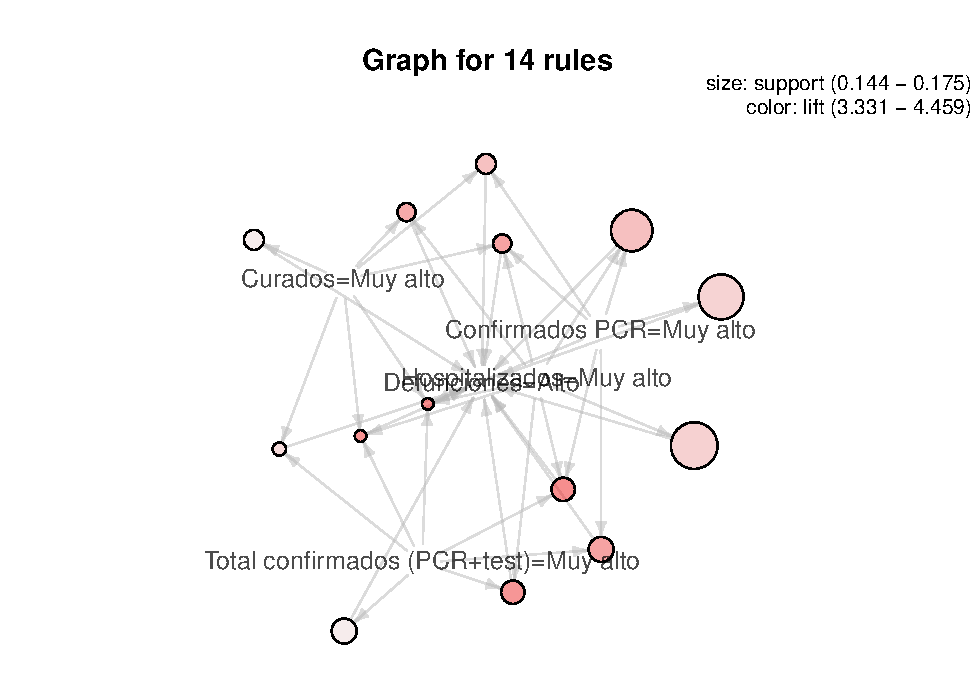
\includegraphics{bookdown-demo_files/figure-latex/unnamed-chunk-8-1.pdf}

As we can see, most of the rules give us very obvious information such as ** \{Hospitalized = Very high, Total confirmed (PCR + test) = Very high\} =\textgreater{} \{Deaths = High\} **
It can also be interpreted as that there is a strong correlation between the different columns, but it is more efficient to apply regression methods in these cases in which we have quantitative variables.

\hypertarget{fcar}{%
\chapter{fcaR}\label{fcar}}

\begin{Shaded}
\begin{Highlighting}[]
\KeywordTok{library}\NormalTok{(}\StringTok{"fcaR"}\NormalTok{)}
\KeywordTok{library}\NormalTok{(}\StringTok{"arules"}\NormalTok{)}
\NormalTok{covid \textless{}{-}}\StringTok{ }\KeywordTok{read.csv}\NormalTok{(}\StringTok{"COVID.csv"}\NormalTok{, }\DataTypeTok{header =} \OtherTok{TRUE}\NormalTok{, }\DataTypeTok{sep =} \StringTok{","}\NormalTok{)}
\KeywordTok{head}\NormalTok{(covid)}
\end{Highlighting}
\end{Shaded}

\begin{verbatim}
##   ï..Fecha.declaración Territorio Confirmados.PCR Hospitalizados UCI Curados
## 1                    87          1               9              6   0      26
## 2                    87          2               1              2   0       4
## 3                    87          3               0              0   0       1
## 4                    87          4               0              1   0      11
## 5                    87          5               1              1   0       0
## 6                    87          6               5              2   0       1
##   Defunciones Total.confirmados..PCR.test.
## 1           0                           64
## 2           0                            7
## 3           0                            1
## 4           0                           14
## 5           0                            1
## 6           0                            9
\end{verbatim}

\begin{Shaded}
\begin{Highlighting}[]
\NormalTok{fc\_covid \textless{}{-}}\StringTok{ }\NormalTok{FormalContext}\OperatorTok{$}\KeywordTok{new}\NormalTok{(covid)}
\KeywordTok{print}\NormalTok{(fc\_covid)}
\end{Highlighting}
\end{Shaded}

\begin{verbatim}
## Warning: Too many attributes, output will be truncated.
\end{verbatim}

\begin{verbatim}
## FormalContext with 687 objects and 8 attributes.
## Attributes' names are: ï..Fecha.declaración, Territorio, Confirmados.PCR,
##   Hospitalizados, UCI, Curados, ...
## Matrix:
##      ï..Fecha.declaración Territorio Confirmados.PCR Hospitalizados UCI
## [1,]                    87          1               9              6   0
## [2,]                    87          2               1              2   0
## [3,]                    87          3               0              0   0
## [4,]                    87          4               0              1   0
## [5,]                    87          5               1              1   0
## [6,]                    87          6               5              2   0
##      Curados Defunciones
## [1,]      26           0
## [2,]       4           0
## [3,]       1           0
## [4,]      11           0
## [5,]       0           0
## [6,]       1           0
\end{verbatim}

\begin{Shaded}
\begin{Highlighting}[]
\NormalTok{fc\_covid}\OperatorTok{$}\KeywordTok{plot}\NormalTok{()}
\end{Highlighting}
\end{Shaded}

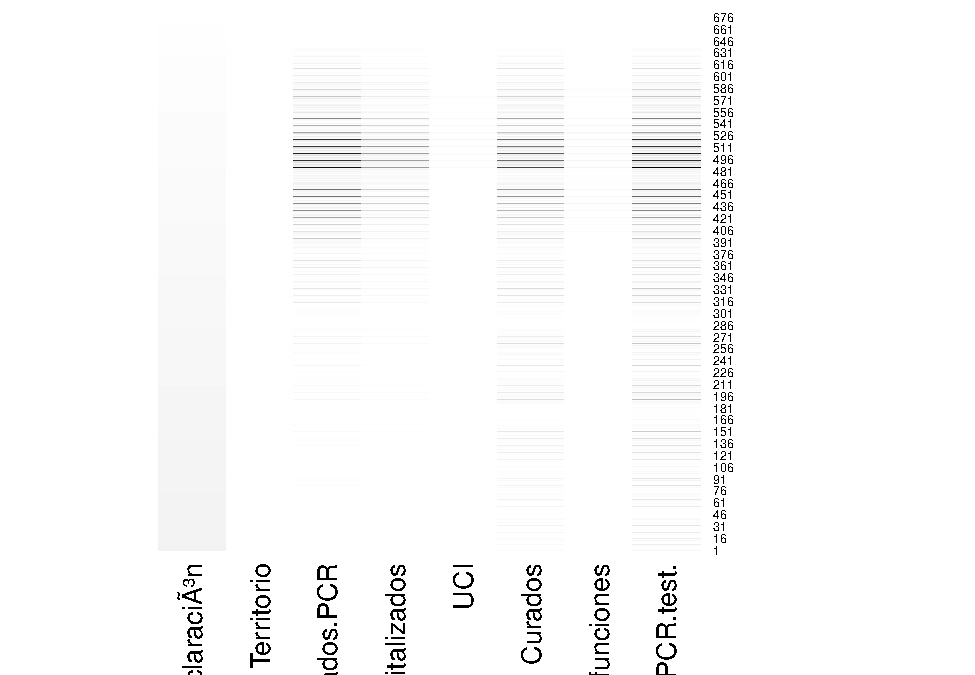
\includegraphics{bookdown-demo_files/figure-latex/unnamed-chunk-9-1.pdf}

\begin{Shaded}
\begin{Highlighting}[]
\NormalTok{fc\_covid}\OperatorTok{$}\NormalTok{objects}
\end{Highlighting}
\end{Shaded}

\begin{verbatim}
##   [1] "1"   "2"   "3"   "4"   "5"   "6"   "7"   "8"   "9"   "10"  "11"  "12" 
##  [13] "13"  "14"  "15"  "16"  "17"  "18"  "19"  "20"  "21"  "22"  "23"  "24" 
##  [25] "25"  "26"  "27"  "28"  "29"  "30"  "31"  "32"  "33"  "34"  "35"  "36" 
##  [37] "37"  "38"  "39"  "40"  "41"  "42"  "43"  "44"  "45"  "46"  "47"  "48" 
##  [49] "49"  "50"  "51"  "52"  "53"  "54"  "55"  "56"  "57"  "58"  "59"  "60" 
##  [61] "61"  "62"  "63"  "64"  "65"  "66"  "67"  "68"  "69"  "70"  "71"  "72" 
##  [73] "73"  "74"  "75"  "76"  "77"  "78"  "79"  "80"  "81"  "82"  "83"  "84" 
##  [85] "85"  "86"  "87"  "88"  "89"  "90"  "91"  "92"  "93"  "94"  "95"  "96" 
##  [97] "97"  "98"  "99"  "100" "101" "102" "103" "104" "105" "106" "107" "108"
## [109] "109" "110" "111" "112" "113" "114" "115" "116" "117" "118" "119" "120"
## [121] "121" "122" "123" "124" "125" "126" "127" "128" "129" "130" "131" "132"
## [133] "133" "134" "135" "136" "137" "138" "139" "140" "141" "142" "143" "144"
## [145] "145" "146" "147" "148" "149" "150" "151" "152" "153" "154" "155" "156"
## [157] "157" "158" "159" "160" "161" "162" "163" "164" "165" "166" "167" "168"
## [169] "169" "170" "171" "172" "173" "174" "175" "176" "177" "178" "179" "180"
## [181] "181" "182" "183" "184" "185" "186" "187" "188" "189" "190" "191" "192"
## [193] "193" "194" "195" "196" "197" "198" "199" "200" "201" "202" "203" "204"
## [205] "205" "206" "207" "208" "209" "210" "211" "212" "213" "214" "215" "216"
## [217] "217" "218" "219" "220" "221" "222" "223" "224" "225" "226" "227" "228"
## [229] "229" "230" "231" "232" "233" "234" "235" "236" "237" "238" "239" "240"
## [241] "241" "242" "243" "244" "245" "246" "247" "248" "249" "250" "251" "252"
## [253] "253" "254" "255" "256" "257" "258" "259" "260" "261" "262" "263" "264"
## [265] "265" "266" "267" "268" "269" "270" "271" "272" "273" "274" "275" "276"
## [277] "277" "278" "279" "280" "281" "282" "283" "284" "285" "286" "287" "288"
## [289] "289" "290" "291" "292" "293" "294" "295" "296" "297" "298" "299" "300"
## [301] "301" "302" "303" "304" "305" "306" "307" "308" "309" "310" "311" "312"
## [313] "313" "314" "315" "316" "317" "318" "319" "320" "321" "322" "323" "324"
## [325] "325" "326" "327" "328" "329" "330" "331" "332" "333" "334" "335" "336"
## [337] "337" "338" "339" "340" "341" "342" "343" "344" "345" "346" "347" "348"
## [349] "349" "350" "351" "352" "353" "354" "355" "356" "357" "358" "359" "360"
## [361] "361" "362" "363" "364" "365" "366" "367" "368" "369" "370" "371" "372"
## [373] "373" "374" "375" "376" "377" "378" "379" "380" "381" "382" "383" "384"
## [385] "385" "386" "387" "388" "389" "390" "391" "392" "393" "394" "395" "396"
## [397] "397" "398" "399" "400" "401" "402" "403" "404" "405" "406" "407" "408"
## [409] "409" "410" "411" "412" "413" "414" "415" "416" "417" "418" "419" "420"
## [421] "421" "422" "423" "424" "425" "426" "427" "428" "429" "430" "431" "432"
## [433] "433" "434" "435" "436" "437" "438" "439" "440" "441" "442" "443" "444"
## [445] "445" "446" "447" "448" "449" "450" "451" "452" "453" "454" "455" "456"
## [457] "457" "458" "459" "460" "461" "462" "463" "464" "465" "466" "467" "468"
## [469] "469" "470" "471" "472" "473" "474" "475" "476" "477" "478" "479" "480"
## [481] "481" "482" "483" "484" "485" "486" "487" "488" "489" "490" "491" "492"
## [493] "493" "494" "495" "496" "497" "498" "499" "500" "501" "502" "503" "504"
## [505] "505" "506" "507" "508" "509" "510" "511" "512" "513" "514" "515" "516"
## [517] "517" "518" "519" "520" "521" "522" "523" "524" "525" "526" "527" "528"
## [529] "529" "530" "531" "532" "533" "534" "535" "536" "537" "538" "539" "540"
## [541] "541" "542" "543" "544" "545" "546" "547" "548" "549" "550" "551" "552"
## [553] "553" "554" "555" "556" "557" "558" "559" "560" "561" "562" "563" "564"
## [565] "565" "566" "567" "568" "569" "570" "571" "572" "573" "574" "575" "576"
## [577] "577" "578" "579" "580" "581" "582" "583" "584" "585" "586" "587" "588"
## [589] "589" "590" "591" "592" "593" "594" "595" "596" "597" "598" "599" "600"
## [601] "601" "602" "603" "604" "605" "606" "607" "608" "609" "610" "611" "612"
## [613] "613" "614" "615" "616" "617" "618" "619" "620" "621" "622" "623" "624"
## [625] "625" "626" "627" "628" "629" "630" "631" "632" "633" "634" "635" "636"
## [637] "637" "638" "639" "640" "641" "642" "643" "644" "645" "646" "647" "648"
## [649] "649" "650" "651" "652" "653" "654" "655" "656" "657" "658" "659" "660"
## [661] "661" "662" "663" "664" "665" "666" "667" "668" "669" "670" "671" "672"
## [673] "673" "674" "675" "676" "677" "678" "679" "680" "681" "682" "683" "684"
## [685] "685" "686" "687"
\end{verbatim}

We find the implications and the concepts.

\begin{Shaded}
\begin{Highlighting}[]
\NormalTok{S \textless{}{-}}\StringTok{ }\NormalTok{SparseSet}\OperatorTok{$}\KeywordTok{new}\NormalTok{(}\DataTypeTok{attributes =}\NormalTok{ fc\_covid}\OperatorTok{$}\NormalTok{objects)}
\NormalTok{fc\_covid}\OperatorTok{$}\KeywordTok{find\_implications}\NormalTok{()}
\NormalTok{fc\_covid}\OperatorTok{$}\NormalTok{implications}
\end{Highlighting}
\end{Shaded}

As we can see, there are no implications. Maybe this could be fixed discretizing the columns with data about the patients and healed.

\begin{Shaded}
\begin{Highlighting}[]
\NormalTok{fc\_covid}\OperatorTok{$}\KeywordTok{find\_concepts}\NormalTok{()}
\NormalTok{fc\_covid}\OperatorTok{$}\NormalTok{concepts}
\end{Highlighting}
\end{Shaded}

\begin{verbatim}
## A set of 24 concepts:
## 1: ({1, 2, 3, 4, 5, 6, 7, 8, 9, 10, 11, 12, 13, 14, 15, 16, 17, 18, 19, 20, 21, 22, 23, 24, 25, 26, 27, 28, 29, 30, 31, 32, 33, 34, 35, 36, 37, 38, 39, 40, 41, 42, 43, 44, 45, 46, 47, 48, 49, 50, 51, 52, 53, 54, 55, 56, 57, 58, 59, 60, 61, 62, 63, 64, 65, 66, 67, 68, 69, 70, 71, 72, 73, 74, 75, 76, 77, 78, 79, 80, 81, 82, 83, 84, 85, 86, 87, 88, 89, 90, 91, 92, 93, 94, 95, 96, 97, 98, 99, 100, 101, 102, 103, 104, 105, 106, 107, 108, 109, 110, 111, 112, 113, 114, 115, 116, 117, 118, 119, 120, 121, 122, 123, 124, 125, 126, 127, 128, 129, 130, 131, 132, 133, 134, 135, 136, 137, 138, 139, 140, 141, 142, 143, 144, 145, 146, 147, 148, 149, 150, 151, 152, 153, 154, 155, 156, 157, 158, 159, 160, 161, 162, 163, 164, 165, 166, 167, 168, 169, 170, 171, 172, 173, 174, 175, 176, 177, 178, 179, 180, 181, 182, 183, 184, 185, 186, 187, 188, 189, 190, 191, 192, 193, 194, 195, 196, 197, 198, 199, 200, 201, 202, 203, 204, 205, 206, 207, 208, 209, 210, 211, 212, 213, 214, 215, 216, 217, 218, 219, 220, 221, 222, 223, 224, 225, 226, 227, 228, 229, 230, 231, 232, 233, 234, 235, 236, 237, 238, 239, 240, 241, 242, 243, 244, 245, 246, 247, 248, 249, 250, 251, 252, 253, 254, 255, 256, 257, 258, 259, 260, 261, 262, 263, 264, 265, 266, 267, 268, 269, 270, 271, 272, 273, 274, 275, 276, 277, 278, 279, 280, 281, 282, 283, 284, 285, 286, 287, 288, 289, 290, 291, 292, 293, 294, 295, 296, 297, 298, 299, 300, 301, 302, 303, 304, 305, 306, 307, 308, 309, 310, 311, 312, 313, 314, 315, 316, 317, 318, 319, 320, 321, 322, 323, 324, 325, 326, 327, 328, 329, 330, 331, 332, 333, 334, 335, 336, 337, 338, 339, 340, 341, 342, 343, 344, 345, 346, 347, 348, 349, 350, 351, 352, 353, 354, 355, 356, 357, 358, 359, 360, 361, 362, 363, 364, 365, 366, 367, 368, 369, 370, 371, 372, 373, 374, 375, 376, 377, 378, 379, 380, 381, 382, 383, 384, 385, 386, 387, 388, 389, 390, 391, 392, 393, 394, 395, 396, 397, 398, 399, 400, 401, 402, 403, 404, 405, 406, 407, 408, 409, 410, 411, 412, 413, 414, 415, 416, 417, 418, 419, 420, 421, 422, 423, 424, 425, 426, 427, 428, 429, 430, 431, 432, 433, 434, 435, 436, 437, 438, 439, 440, 441, 442, 443, 444, 445, 446, 447, 448, 449, 450, 451, 452, 453, 454, 455, 456, 457, 458, 459, 460, 461, 462, 463, 464, 465, 466, 467, 468, 469, 470, 471, 472, 473, 474, 475, 476, 477, 478, 479, 480, 481, 482, 483, 484, 485, 486, 487, 488, 489, 490, 491, 492, 493, 494, 495, 496, 497, 498, 499, 500, 501, 502, 503, 504, 505, 506, 507, 508, 509, 510, 511, 512, 513, 514, 515, 516, 517, 518, 519, 520, 521, 522, 523, 524, 525, 526, 527, 528, 529, 530, 531, 532, 533, 534, 535, 536, 537, 538, 539, 540, 541, 542, 543, 544, 545, 546, 547, 548, 549, 550, 551, 552, 553, 554, 555, 556, 557, 558, 559, 560, 561, 562, 563, 564, 565, 566, 567, 568, 569, 570, 571, 572, 573, 574, 575, 576, 577, 578, 579, 580, 581, 582, 583, 584, 585, 586, 587, 588, 589, 590, 591, 592, 593, 594, 595, 596, 597, 598, 599, 600, 601, 602, 603, 604, 605, 606, 607, 608, 609, 610, 611, 612, 613, 614, 615, 616, 617, 618, 619, 620, 621, 622, 623, 624, 625, 626, 627, 628, 629, 630, 631, 632, 633, 634, 635, 636, 637, 638, 639, 640, 641, 642, 643, 644, 645, 646, 647, 648, 649, 650, 651, 652, 653, 654, 655, 656, 657, 658, 659, 660, 661, 662, 663, 664, 665, 666, 667, 668, 669, 670, 671, 672, 673, 674, 675, 676, 677, 678, 679, 680, 681, 682, 683, 684, 685, 686, 687}, {ï..Fecha.declaración, Territorio, Total.confirmados..PCR.test.})
## 2: ({33, 36, 74, 75, 78, 81, 101, 104, 105, 106, 107, 116, 123, 125, 129, 143, 144, 147, 152, 156, 158, 167, 171, 174, 180, 183, 189, 192, 196, 200, 201, 205, 207, 210, 215, 217, 218, 219, 221, 224, 228, 229, 233, 236, 239, 243, 245, 249, 254, 256, 258, 262, 263, 265, 266, 267, 269, 270, 271, 272, 274, 276, 278, 279, 280, 281, 282, 283, 288, 290, 291, 292, 294, 297, 298, 299, 301, 304, 305, 306, 308, 311, 312, 313, 315, 317, 319, 323, 324, 326, 329, 330, 331, 332, 333, 335, 337, 339, 340, 341, 342, 343, 344, 346, 348, 350, 351, 353, 354, 355, 357, 358, 359, 360, 362, 364, 365, 366, 367, 368, 369, 370, 372, 373, 376, 377, 378, 380, 381, 382, 383, 384, 385, 386, 387, 388, 389, 390, 391, 392, 393, 394, 395, 396, 400, 402, 403, 404, 405, 408, 409, 410, 411, 412, 413, 414, 418, 419, 420, 421, 422, 423, 424, 425, 426, 427, 428, 429, 430, 431, 432, 433, 434, 435, 436, 437, 438, 439, 440, 441, 442, 443, 444, 445, 447, 448, 449, 450, 451, 452, 453, 454, 455, 456, 457, 458, 459, 460, 461, 462, 463, 464, 465, 466, 467, 468, 469, 470, 471, 472, 473, 474, 475, 476, 477, 479, 480, 481, 482, 483, 484, 485, 486, 487, 488, 489, 490, 491, 492, 493, 494, 495, 496, 497, 498, 499, 500, 501, 502, 503, 504, 505, 506, 507, 508, 509, 510, 511, 512, 513, 514, 515, 516, 517, 518, 519, 520, 521, 522, 523, 524, 525, 526, 527, 528, 529, 530, 531, 532, 533, 534, 535, 536, 537, 538, 539, 540, 541, 542, 543, 544, 545, 546, 547, 548, 549, 550, 551, 552, 553, 554, 555, 556, 557, 558, 560, 562, 563, 564, 565, 566, 567, 568, 570, 571, 573, 574, 575, 576, 577, 578, 579, 580, 582, 583, 584, 585, 586, 587, 588, 589, 590, 591, 592, 593, 594, 597, 598, 600, 601, 602, 603, 607, 609, 610, 611, 612, 613, 614, 615, 616, 617, 618, 619, 620, 621, 623, 624, 626, 627, 629, 631, 634, 635, 637, 642, 644, 647, 648, 651, 652, 663, 665, 667, 668, 672, 673}, {ï..Fecha.declaración, Territorio, Defunciones, Total.confirmados..PCR.test.})
## 3: ({1, 2, 3, 4, 6, 7, 8, 9, 10, 11, 12, 13, 14, 15, 16, 17, 18, 19, 20, 21, 22, 23, 24, 25, 26, 27, 28, 29, 30, 31, 32, 33, 34, 35, 36, 37, 39, 40, 41, 42, 43, 44, 45, 47, 48, 49, 50, 51, 52, 53, 55, 56, 57, 58, 59, 60, 61, 62, 63, 64, 65, 66, 67, 68, 69, 70, 71, 72, 73, 74, 75, 76, 77, 78, 79, 80, 81, 82, 83, 84, 85, 86, 87, 88, 89, 90, 91, 92, 93, 94, 95, 96, 98, 99, 100, 101, 102, 103, 106, 107, 108, 109, 110, 111, 112, 114, 115, 116, 117, 118, 119, 120, 121, 123, 124, 125, 126, 127, 128, 129, 130, 131, 132, 133, 134, 135, 136, 137, 138, 139, 140, 141, 142, 143, 144, 145, 146, 147, 148, 149, 150, 151, 152, 153, 154, 155, 156, 157, 158, 159, 160, 161, 163, 164, 165, 166, 167, 168, 169, 170, 172, 173, 174, 177, 178, 179, 181, 182, 183, 184, 185, 186, 187, 188, 189, 190, 191, 192, 193, 194, 195, 196, 197, 198, 199, 200, 201, 202, 203, 204, 205, 206, 207, 208, 209, 210, 211, 212, 213, 214, 215, 216, 217, 218, 219, 220, 222, 223, 224, 225, 226, 227, 228, 229, 230, 231, 232, 233, 234, 235, 236, 237, 238, 239, 240, 241, 242, 243, 244, 245, 246, 247, 248, 249, 250, 251, 252, 253, 254, 255, 256, 257, 258, 259, 260, 261, 262, 263, 264, 265, 266, 267, 268, 269, 270, 271, 272, 273, 274, 275, 276, 277, 278, 279, 280, 281, 282, 283, 285, 286, 287, 288, 289, 290, 291, 292, 293, 295, 296, 297, 298, 299, 300, 301, 302, 303, 304, 305, 306, 307, 308, 309, 310, 311, 312, 313, 314, 315, 316, 317, 318, 319, 320, 321, 322, 323, 324, 325, 326, 327, 328, 329, 330, 331, 332, 333, 334, 335, 336, 337, 338, 339, 340, 341, 342, 343, 344, 345, 346, 347, 348, 349, 350, 351, 352, 353, 354, 355, 356, 357, 358, 359, 360, 361, 362, 363, 364, 365, 366, 367, 368, 369, 370, 371, 372, 373, 374, 375, 376, 377, 378, 379, 380, 381, 382, 383, 384, 385, 386, 387, 388, 389, 390, 391, 392, 393, 394, 395, 396, 397, 398, 399, 400, 401, 402, 403, 404, 405, 406, 407, 408, 409, 410, 411, 412, 413, 414, 415, 416, 417, 418, 419, 420, 421, 422, 423, 424, 425, 426, 427, 428, 429, 430, 431, 432, 433, 434, 435, 436, 437, 438, 439, 440, 441, 442, 443, 444, 445, 446, 447, 448, 449, 450, 451, 452, 453, 454, 455, 456, 457, 458, 459, 460, 461, 462, 463, 464, 465, 466, 467, 468, 469, 470, 471, 472, 473, 474, 475, 476, 477, 478, 479, 480, 481, 482, 483, 484, 485, 486, 487, 488, 489, 490, 491, 492, 493, 494, 495, 496, 497, 498, 499, 500, 501, 502, 503, 504, 505, 506, 507, 508, 509, 510, 511, 512, 513, 514, 515, 516, 517, 518, 519, 520, 521, 522, 523, 524, 525, 526, 527, 528, 529, 530, 531, 532, 533, 534, 535, 536, 537, 538, 539, 540, 541, 542, 543, 544, 545, 546, 547, 548, 549, 550, 551, 552, 553, 554, 555, 556, 557, 558, 559, 560, 561, 562, 563, 564, 565, 566, 567, 568, 569, 570, 571, 572, 573, 574, 575, 576, 577, 578, 579, 580, 581, 582, 583, 584, 585, 586, 587, 588, 589, 590, 591, 592, 593, 594, 595, 596, 597, 598, 599, 600, 601, 602, 603, 604, 605, 606, 607, 608, 609, 610, 611, 612, 613, 614, 615, 616, 617, 618, 619, 620, 621, 622, 623, 624, 625, 626, 627, 628, 629, 630, 631, 632, 633, 634, 635, 636, 637, 638, 639, 640, 641, 642, 643, 644, 645, 646, 647, 648, 650, 652, 653, 654, 655, 656, 657, 658, 659, 660, 661, 662, 663, 664, 665, 666, 667, 668, 669, 670, 671, 672, 673, 674, 675, 676, 677, 678, 679, 680, 681, 682, 683, 684, 685, 686, 687}, {ï..Fecha.declaración, Territorio, Curados, Total.confirmados..PCR.test.})
## 4: ({33, 36, 74, 75, 78, 81, 101, 106, 107, 116, 123, 125, 129, 143, 144, 147, 152, 156, 158, 167, 174, 183, 189, 192, 196, 200, 201, 205, 207, 210, 215, 217, 218, 219, 224, 228, 229, 233, 236, 239, 243, 245, 249, 254, 256, 258, 262, 263, 265, 266, 267, 269, 270, 271, 272, 274, 276, 278, 279, 280, 281, 282, 283, 288, 290, 291, 292, 297, 298, 299, 301, 304, 305, 306, 308, 311, 312, 313, 315, 317, 319, 323, 324, 326, 329, 330, 331, 332, 333, 335, 337, 339, 340, 341, 342, 343, 344, 346, 348, 350, 351, 353, 354, 355, 357, 358, 359, 360, 362, 364, 365, 366, 367, 368, 369, 370, 372, 373, 376, 377, 378, 380, 381, 382, 383, 384, 385, 386, 387, 388, 389, 390, 391, 392, 393, 394, 395, 396, 400, 402, 403, 404, 405, 408, 409, 410, 411, 412, 413, 414, 418, 419, 420, 421, 422, 423, 424, 425, 426, 427, 428, 429, 430, 431, 432, 433, 434, 435, 436, 437, 438, 439, 440, 441, 442, 443, 444, 445, 447, 448, 449, 450, 451, 452, 453, 454, 455, 456, 457, 458, 459, 460, 461, 462, 463, 464, 465, 466, 467, 468, 469, 470, 471, 472, 473, 474, 475, 476, 477, 479, 480, 481, 482, 483, 484, 485, 486, 487, 488, 489, 490, 491, 492, 493, 494, 495, 496, 497, 498, 499, 500, 501, 502, 503, 504, 505, 506, 507, 508, 509, 510, 511, 512, 513, 514, 515, 516, 517, 518, 519, 520, 521, 522, 523, 524, 525, 526, 527, 528, 529, 530, 531, 532, 533, 534, 535, 536, 537, 538, 539, 540, 541, 542, 543, 544, 545, 546, 547, 548, 549, 550, 551, 552, 553, 554, 555, 556, 557, 558, 560, 562, 563, 564, 565, 566, 567, 568, 570, 571, 573, 574, 575, 576, 577, 578, 579, 580, 582, 583, 584, 585, 586, 587, 588, 589, 590, 591, 592, 593, 594, 597, 598, 600, 601, 602, 603, 607, 609, 610, 611, 612, 613, 614, 615, 616, 617, 618, 619, 620, 621, 623, 624, 626, 627, 629, 631, 634, 635, 637, 642, 644, 647, 648, 652, 663, 665, 667, 668, 672, 673}, {ï..Fecha.declaración, Territorio, Curados, Defunciones, Total.confirmados..PCR.test.})
## 5: ({1, 2, 4, 5, 6, 9, 12, 14, 15, 16, 17, 18, 19, 20, 21, 22, 24, 26, 28, 30, 32, 33, 36, 37, 40, 49, 50, 54, 57, 58, 60, 61, 63, 64, 66, 67, 68, 71, 74, 75, 77, 78, 81, 82, 83, 84, 87, 89, 91, 92, 93, 94, 95, 96, 98, 99, 101, 102, 103, 104, 105, 106, 107, 108, 109, 111, 114, 115, 116, 117, 118, 120, 122, 123, 124, 125, 128, 129, 131, 133, 134, 135, 137, 138, 140, 141, 142, 143, 144, 145, 147, 149, 150, 151, 152, 154, 156, 158, 159, 160, 161, 162, 163, 164, 165, 166, 167, 171, 173, 174, 178, 180, 183, 184, 185, 186, 187, 189, 190, 192, 194, 195, 196, 199, 200, 201, 202, 203, 204, 205, 207, 208, 209, 210, 211, 213, 214, 215, 216, 217, 218, 219, 221, 223, 224, 225, 226, 227, 228, 229, 230, 231, 232, 233, 234, 235, 236, 237, 238, 239, 240, 241, 243, 244, 245, 246, 247, 249, 251, 252, 253, 254, 255, 256, 258, 259, 260, 261, 262, 263, 265, 266, 267, 268, 269, 270, 271, 272, 274, 275, 276, 278, 279, 280, 281, 282, 283, 285, 286, 287, 288, 290, 291, 292, 293, 294, 295, 297, 298, 299, 300, 301, 302, 303, 304, 305, 306, 307, 308, 310, 311, 312, 313, 314, 315, 316, 317, 318, 319, 320, 321, 322, 323, 324, 325, 326, 327, 328, 329, 330, 331, 332, 333, 334, 335, 336, 337, 338, 339, 340, 341, 342, 343, 344, 345, 346, 347, 348, 349, 350, 351, 352, 353, 354, 355, 356, 357, 358, 359, 360, 361, 362, 363, 364, 365, 366, 367, 368, 369, 371, 372, 373, 374, 375, 376, 377, 378, 379, 380, 381, 382, 383, 384, 385, 386, 387, 388, 389, 390, 391, 392, 393, 394, 395, 396, 397, 398, 399, 400, 402, 403, 404, 405, 406, 407, 408, 409, 410, 411, 412, 413, 414, 415, 416, 417, 418, 419, 420, 421, 422, 423, 424, 425, 426, 427, 428, 429, 430, 431, 432, 433, 434, 435, 436, 437, 438, 439, 440, 441, 442, 443, 444, 445, 446, 447, 448, 449, 450, 451, 452, 453, 454, 455, 456, 457, 458, 459, 460, 461, 462, 463, 464, 465, 466, 467, 468, 469, 470, 471, 472, 473, 474, 475, 476, 477, 478, 479, 480, 481, 482, 483, 484, 485, 486, 487, 488, 489, 490, 491, 492, 493, 494, 495, 496, 497, 498, 499, 500, 501, 502, 503, 504, 505, 506, 507, 508, 509, 510, 511, 512, 513, 514, 515, 516, 517, 518, 519, 520, 521, 522, 523, 524, 525, 526, 527, 528, 529, 530, 531, 532, 533, 534, 535, 536, 537, 538, 539, 540, 541, 542, 543, 544, 545, 546, 547, 548, 549, 550, 551, 552, 553, 554, 555, 556, 557, 558, 559, 560, 561, 562, 563, 564, 565, 566, 567, 568, 569, 570, 571, 573, 574, 575, 576, 577, 578, 579, 580, 581, 582, 583, 584, 585, 586, 587, 588, 589, 590, 591, 592, 593, 594, 596, 597, 598, 599, 600, 601, 602, 603, 604, 605, 606, 607, 609, 610, 611, 612, 613, 614, 615, 616, 617, 618, 619, 620, 621, 622, 623, 624, 626, 627, 628, 629, 631, 632, 633, 634, 635, 636, 637, 638, 639, 640, 641, 642, 643, 644, 647, 648, 649, 651, 652, 653, 656, 657, 658, 661, 663, 664, 665, 666, 667, 668, 670, 671, 672, 673, 677, 678, 679, 681, 683, 684, 686, 687}, {ï..Fecha.declaración, Territorio, Hospitalizados, Total.confirmados..PCR.test.})
## 6: ({33, 36, 74, 75, 78, 81, 101, 104, 105, 106, 107, 116, 123, 125, 129, 143, 144, 147, 152, 156, 158, 167, 171, 174, 180, 183, 189, 192, 196, 200, 201, 205, 207, 210, 215, 217, 218, 219, 221, 224, 228, 229, 233, 236, 239, 243, 245, 249, 254, 256, 258, 262, 263, 265, 266, 267, 269, 270, 271, 272, 274, 276, 278, 279, 280, 281, 282, 283, 288, 290, 291, 292, 294, 297, 298, 299, 301, 304, 305, 306, 308, 311, 312, 313, 315, 317, 319, 323, 324, 326, 329, 330, 331, 332, 333, 335, 337, 339, 340, 341, 342, 343, 344, 346, 348, 350, 351, 353, 354, 355, 357, 358, 359, 360, 362, 364, 365, 366, 367, 368, 369, 372, 373, 376, 377, 378, 380, 381, 382, 383, 384, 385, 386, 387, 388, 389, 390, 391, 392, 393, 394, 395, 396, 400, 402, 403, 404, 405, 408, 409, 410, 411, 412, 413, 414, 418, 419, 420, 421, 422, 423, 424, 425, 426, 427, 428, 429, 430, 431, 432, 433, 434, 435, 436, 437, 438, 439, 440, 441, 442, 443, 444, 445, 447, 448, 449, 450, 451, 452, 453, 454, 455, 456, 457, 458, 459, 460, 461, 462, 463, 464, 465, 466, 467, 468, 469, 470, 471, 472, 473, 474, 475, 476, 477, 479, 480, 481, 482, 483, 484, 485, 486, 487, 488, 489, 490, 491, 492, 493, 494, 495, 496, 497, 498, 499, 500, 501, 502, 503, 504, 505, 506, 507, 508, 509, 510, 511, 512, 513, 514, 515, 516, 517, 518, 519, 520, 521, 522, 523, 524, 525, 526, 527, 528, 529, 530, 531, 532, 533, 534, 535, 536, 537, 538, 539, 540, 541, 542, 543, 544, 545, 546, 547, 548, 549, 550, 551, 552, 553, 554, 555, 556, 557, 558, 560, 562, 563, 564, 565, 566, 567, 568, 570, 571, 573, 574, 575, 576, 577, 578, 579, 580, 582, 583, 584, 585, 586, 587, 588, 589, 590, 591, 592, 593, 594, 597, 598, 600, 601, 602, 603, 607, 609, 610, 611, 612, 613, 614, 615, 616, 617, 618, 619, 620, 621, 623, 624, 626, 627, 629, 631, 634, 635, 637, 642, 644, 647, 648, 651, 652, 663, 665, 667, 668, 672, 673}, {ï..Fecha.declaración, Territorio, Hospitalizados, Defunciones, Total.confirmados..PCR.test.})
## 7: ({1, 2, 4, 6, 9, 12, 14, 15, 16, 17, 18, 19, 20, 21, 22, 24, 26, 28, 30, 32, 33, 36, 37, 40, 49, 50, 57, 58, 60, 61, 63, 64, 66, 67, 68, 71, 74, 75, 77, 78, 81, 82, 83, 84, 87, 89, 91, 92, 93, 94, 95, 96, 98, 99, 101, 102, 103, 106, 107, 108, 109, 111, 114, 115, 116, 117, 118, 120, 123, 124, 125, 128, 129, 131, 133, 134, 135, 137, 138, 140, 141, 142, 143, 144, 145, 147, 149, 150, 151, 152, 154, 156, 158, 159, 160, 161, 163, 164, 165, 166, 167, 173, 174, 178, 183, 184, 185, 186, 187, 189, 190, 192, 194, 195, 196, 199, 200, 201, 202, 203, 204, 205, 207, 208, 209, 210, 211, 213, 214, 215, 216, 217, 218, 219, 223, 224, 225, 226, 227, 228, 229, 230, 231, 232, 233, 234, 235, 236, 237, 238, 239, 240, 241, 243, 244, 245, 246, 247, 249, 251, 252, 253, 254, 255, 256, 258, 259, 260, 261, 262, 263, 265, 266, 267, 268, 269, 270, 271, 272, 274, 275, 276, 278, 279, 280, 281, 282, 283, 285, 286, 287, 288, 290, 291, 292, 293, 295, 297, 298, 299, 300, 301, 302, 303, 304, 305, 306, 307, 308, 310, 311, 312, 313, 314, 315, 316, 317, 318, 319, 320, 321, 322, 323, 324, 325, 326, 327, 328, 329, 330, 331, 332, 333, 334, 335, 336, 337, 338, 339, 340, 341, 342, 343, 344, 345, 346, 347, 348, 349, 350, 351, 352, 353, 354, 355, 356, 357, 358, 359, 360, 361, 362, 363, 364, 365, 366, 367, 368, 369, 371, 372, 373, 374, 375, 376, 377, 378, 379, 380, 381, 382, 383, 384, 385, 386, 387, 388, 389, 390, 391, 392, 393, 394, 395, 396, 397, 398, 399, 400, 402, 403, 404, 405, 406, 407, 408, 409, 410, 411, 412, 413, 414, 415, 416, 417, 418, 419, 420, 421, 422, 423, 424, 425, 426, 427, 428, 429, 430, 431, 432, 433, 434, 435, 436, 437, 438, 439, 440, 441, 442, 443, 444, 445, 446, 447, 448, 449, 450, 451, 452, 453, 454, 455, 456, 457, 458, 459, 460, 461, 462, 463, 464, 465, 466, 467, 468, 469, 470, 471, 472, 473, 474, 475, 476, 477, 478, 479, 480, 481, 482, 483, 484, 485, 486, 487, 488, 489, 490, 491, 492, 493, 494, 495, 496, 497, 498, 499, 500, 501, 502, 503, 504, 505, 506, 507, 508, 509, 510, 511, 512, 513, 514, 515, 516, 517, 518, 519, 520, 521, 522, 523, 524, 525, 526, 527, 528, 529, 530, 531, 532, 533, 534, 535, 536, 537, 538, 539, 540, 541, 542, 543, 544, 545, 546, 547, 548, 549, 550, 551, 552, 553, 554, 555, 556, 557, 558, 559, 560, 561, 562, 563, 564, 565, 566, 567, 568, 569, 570, 571, 573, 574, 575, 576, 577, 578, 579, 580, 581, 582, 583, 584, 585, 586, 587, 588, 589, 590, 591, 592, 593, 594, 596, 597, 598, 599, 600, 601, 602, 603, 604, 605, 606, 607, 609, 610, 611, 612, 613, 614, 615, 616, 617, 618, 619, 620, 621, 622, 623, 624, 626, 627, 628, 629, 631, 632, 633, 634, 635, 636, 637, 638, 639, 640, 641, 642, 643, 644, 647, 648, 652, 653, 656, 657, 658, 661, 663, 664, 665, 666, 667, 668, 670, 671, 672, 673, 677, 678, 679, 681, 683, 684, 686, 687}, {ï..Fecha.declaración, Territorio, Hospitalizados, Curados, Total.confirmados..PCR.test.})
## 8: ({33, 36, 74, 75, 78, 81, 101, 106, 107, 116, 123, 125, 129, 143, 144, 147, 152, 156, 158, 167, 174, 183, 189, 192, 196, 200, 201, 205, 207, 210, 215, 217, 218, 219, 224, 228, 229, 233, 236, 239, 243, 245, 249, 254, 256, 258, 262, 263, 265, 266, 267, 269, 270, 271, 272, 274, 276, 278, 279, 280, 281, 282, 283, 288, 290, 291, 292, 297, 298, 299, 301, 304, 305, 306, 308, 311, 312, 313, 315, 317, 319, 323, 324, 326, 329, 330, 331, 332, 333, 335, 337, 339, 340, 341, 342, 343, 344, 346, 348, 350, 351, 353, 354, 355, 357, 358, 359, 360, 362, 364, 365, 366, 367, 368, 369, 372, 373, 376, 377, 378, 380, 381, 382, 383, 384, 385, 386, 387, 388, 389, 390, 391, 392, 393, 394, 395, 396, 400, 402, 403, 404, 405, 408, 409, 410, 411, 412, 413, 414, 418, 419, 420, 421, 422, 423, 424, 425, 426, 427, 428, 429, 430, 431, 432, 433, 434, 435, 436, 437, 438, 439, 440, 441, 442, 443, 444, 445, 447, 448, 449, 450, 451, 452, 453, 454, 455, 456, 457, 458, 459, 460, 461, 462, 463, 464, 465, 466, 467, 468, 469, 470, 471, 472, 473, 474, 475, 476, 477, 479, 480, 481, 482, 483, 484, 485, 486, 487, 488, 489, 490, 491, 492, 493, 494, 495, 496, 497, 498, 499, 500, 501, 502, 503, 504, 505, 506, 507, 508, 509, 510, 511, 512, 513, 514, 515, 516, 517, 518, 519, 520, 521, 522, 523, 524, 525, 526, 527, 528, 529, 530, 531, 532, 533, 534, 535, 536, 537, 538, 539, 540, 541, 542, 543, 544, 545, 546, 547, 548, 549, 550, 551, 552, 553, 554, 555, 556, 557, 558, 560, 562, 563, 564, 565, 566, 567, 568, 570, 571, 573, 574, 575, 576, 577, 578, 579, 580, 582, 583, 584, 585, 586, 587, 588, 589, 590, 591, 592, 593, 594, 597, 598, 600, 601, 602, 603, 607, 609, 610, 611, 612, 613, 614, 615, 616, 617, 618, 619, 620, 621, 623, 624, 626, 627, 629, 631, 634, 635, 637, 642, 644, 647, 648, 652, 663, 665, 667, 668, 672, 673}, {ï..Fecha.declaración, Territorio, Hospitalizados, Curados, Defunciones, Total.confirmados..PCR.test.})
## 9: ({16, 21, 24, 26, 32, 49, 50, 92, 95, 101, 105, 106, 116, 124, 125, 128, 131, 134, 140, 143, 144, 152, 158, 159, 167, 171, 183, 184, 189, 192, 196, 199, 201, 205, 207, 210, 218, 219, 226, 228, 233, 245, 249, 252, 263, 267, 271, 272, 276, 279, 280, 281, 282, 288, 291, 295, 297, 303, 306, 307, 324, 325, 326, 328, 330, 332, 333, 337, 340, 342, 346, 347, 348, 351, 355, 356, 360, 364, 366, 369, 371, 376, 377, 378, 380, 381, 384, 385, 386, 387, 388, 390, 393, 395, 396, 400, 402, 403, 404, 405, 407, 409, 411, 412, 413, 414, 416, 418, 419, 422, 423, 424, 426, 427, 429, 430, 431, 432, 434, 435, 436, 438, 439, 440, 441, 444, 445, 447, 448, 449, 450, 451, 452, 454, 455, 456, 457, 458, 459, 460, 461, 463, 465, 466, 467, 468, 469, 470, 471, 472, 473, 474, 475, 476, 477, 478, 479, 480, 481, 482, 483, 484, 485, 486, 487, 488, 489, 490, 492, 493, 494, 495, 496, 497, 498, 499, 500, 501, 502, 503, 504, 505, 506, 507, 508, 509, 510, 511, 512, 513, 514, 515, 516, 517, 518, 519, 520, 521, 522, 523, 524, 525, 526, 527, 528, 529, 530, 531, 532, 533, 534, 535, 536, 537, 538, 539, 540, 541, 542, 543, 544, 545, 546, 547, 548, 549, 550, 551, 552, 553, 554, 555, 556, 557, 558, 560, 561, 562, 563, 564, 565, 566, 567, 568, 570, 571, 573, 574, 575, 576, 577, 578, 579, 580, 581, 582, 583, 584, 585, 588, 589, 590, 591, 592, 593, 594, 597, 598, 600, 601, 602, 603, 604, 606, 607, 609, 610, 611, 612, 613, 614, 615, 616, 617, 618, 619, 620, 621, 622, 623, 624, 626, 628, 629, 631, 633, 634, 635, 637, 640, 642, 643, 644, 647, 648, 649, 651, 652, 653, 657, 663, 665, 667, 668, 672, 673}, {ï..Fecha.declaración, Territorio, Hospitalizados, UCI, Total.confirmados..PCR.test.})
## 10: ({101, 105, 106, 116, 125, 143, 144, 152, 158, 167, 171, 183, 189, 192, 196, 201, 205, 207, 210, 218, 219, 228, 233, 245, 249, 263, 267, 271, 272, 276, 279, 280, 281, 282, 288, 291, 297, 306, 324, 326, 330, 332, 333, 337, 340, 342, 346, 348, 351, 355, 360, 364, 366, 369, 376, 377, 378, 380, 381, 384, 385, 386, 387, 388, 390, 393, 395, 396, 400, 402, 403, 404, 405, 409, 411, 412, 413, 414, 418, 419, 422, 423, 424, 426, 427, 429, 430, 431, 432, 434, 435, 436, 438, 439, 440, 441, 444, 445, 447, 448, 449, 450, 451, 452, 454, 455, 456, 457, 458, 459, 460, 461, 463, 465, 466, 467, 468, 469, 470, 471, 472, 473, 474, 475, 476, 477, 479, 480, 481, 482, 483, 484, 485, 486, 487, 488, 489, 490, 492, 493, 494, 495, 496, 497, 498, 499, 500, 501, 502, 503, 504, 505, 506, 507, 508, 509, 510, 511, 512, 513, 514, 515, 516, 517, 518, 519, 520, 521, 522, 523, 524, 525, 526, 527, 528, 529, 530, 531, 532, 533, 534, 535, 536, 537, 538, 539, 540, 541, 542, 543, 544, 545, 546, 547, 548, 549, 550, 551, 552, 553, 554, 555, 556, 557, 558, 560, 562, 563, 564, 565, 566, 567, 568, 570, 571, 573, 574, 575, 576, 577, 578, 579, 580, 582, 583, 584, 585, 588, 589, 590, 591, 592, 593, 594, 597, 598, 600, 601, 602, 603, 607, 609, 610, 611, 612, 613, 614, 615, 616, 617, 618, 619, 620, 621, 623, 624, 626, 629, 631, 634, 635, 637, 642, 644, 647, 648, 651, 652, 663, 665, 667, 668, 672, 673}, {ï..Fecha.declaración, Territorio, Hospitalizados, UCI, Defunciones, Total.confirmados..PCR.test.})
## 11: ({16, 21, 24, 26, 32, 49, 50, 92, 95, 101, 106, 116, 124, 125, 128, 131, 134, 140, 143, 144, 152, 158, 159, 167, 183, 184, 189, 192, 196, 199, 201, 205, 207, 210, 218, 219, 226, 228, 233, 245, 249, 252, 263, 267, 271, 272, 276, 279, 280, 281, 282, 288, 291, 295, 297, 303, 306, 307, 324, 325, 326, 328, 330, 332, 333, 337, 340, 342, 346, 347, 348, 351, 355, 356, 360, 364, 366, 369, 371, 376, 377, 378, 380, 381, 384, 385, 386, 387, 388, 390, 393, 395, 396, 400, 402, 403, 404, 405, 407, 409, 411, 412, 413, 414, 416, 418, 419, 422, 423, 424, 426, 427, 429, 430, 431, 432, 434, 435, 436, 438, 439, 440, 441, 444, 445, 447, 448, 449, 450, 451, 452, 454, 455, 456, 457, 458, 459, 460, 461, 463, 465, 466, 467, 468, 469, 470, 471, 472, 473, 474, 475, 476, 477, 478, 479, 480, 481, 482, 483, 484, 485, 486, 487, 488, 489, 490, 492, 493, 494, 495, 496, 497, 498, 499, 500, 501, 502, 503, 504, 505, 506, 507, 508, 509, 510, 511, 512, 513, 514, 515, 516, 517, 518, 519, 520, 521, 522, 523, 524, 525, 526, 527, 528, 529, 530, 531, 532, 533, 534, 535, 536, 537, 538, 539, 540, 541, 542, 543, 544, 545, 546, 547, 548, 549, 550, 551, 552, 553, 554, 555, 556, 557, 558, 560, 561, 562, 563, 564, 565, 566, 567, 568, 570, 571, 573, 574, 575, 576, 577, 578, 579, 580, 581, 582, 583, 584, 585, 588, 589, 590, 591, 592, 593, 594, 597, 598, 600, 601, 602, 603, 604, 606, 607, 609, 610, 611, 612, 613, 614, 615, 616, 617, 618, 619, 620, 621, 622, 623, 624, 626, 628, 629, 631, 633, 634, 635, 637, 640, 642, 643, 644, 647, 648, 652, 653, 657, 663, 665, 667, 668, 672, 673}, {ï..Fecha.declaración, Territorio, Hospitalizados, UCI, Curados, Total.confirmados..PCR.test.})
## 12: ({101, 106, 116, 125, 143, 144, 152, 158, 167, 183, 189, 192, 196, 201, 205, 207, 210, 218, 219, 228, 233, 245, 249, 263, 267, 271, 272, 276, 279, 280, 281, 282, 288, 291, 297, 306, 324, 326, 330, 332, 333, 337, 340, 342, 346, 348, 351, 355, 360, 364, 366, 369, 376, 377, 378, 380, 381, 384, 385, 386, 387, 388, 390, 393, 395, 396, 400, 402, 403, 404, 405, 409, 411, 412, 413, 414, 418, 419, 422, 423, 424, 426, 427, 429, 430, 431, 432, 434, 435, 436, 438, 439, 440, 441, 444, 445, 447, 448, 449, 450, 451, 452, 454, 455, 456, 457, 458, 459, 460, 461, 463, 465, 466, 467, 468, 469, 470, 471, 472, 473, 474, 475, 476, 477, 479, 480, 481, 482, 483, 484, 485, 486, 487, 488, 489, 490, 492, 493, 494, 495, 496, 497, 498, 499, 500, 501, 502, 503, 504, 505, 506, 507, 508, 509, 510, 511, 512, 513, 514, 515, 516, 517, 518, 519, 520, 521, 522, 523, 524, 525, 526, 527, 528, 529, 530, 531, 532, 533, 534, 535, 536, 537, 538, 539, 540, 541, 542, 543, 544, 545, 546, 547, 548, 549, 550, 551, 552, 553, 554, 555, 556, 557, 558, 560, 562, 563, 564, 565, 566, 567, 568, 570, 571, 573, 574, 575, 576, 577, 578, 579, 580, 582, 583, 584, 585, 588, 589, 590, 591, 592, 593, 594, 597, 598, 600, 601, 602, 603, 607, 609, 610, 611, 612, 613, 614, 615, 616, 617, 618, 619, 620, 621, 623, 624, 626, 629, 631, 634, 635, 637, 642, 644, 647, 648, 652, 663, 665, 667, 668, 672, 673}, {ï..Fecha.declaración, Territorio, Hospitalizados, UCI, Curados, Defunciones, Total.confirmados..PCR.test.})
## 13: ({1, 2, 5, 6, 7, 9, 11, 12, 13, 14, 15, 16, 17, 18, 19, 20, 21, 22, 24, 26, 27, 28, 30, 31, 32, 33, 35, 36, 37, 38, 39, 40, 41, 42, 44, 45, 46, 48, 49, 52, 54, 55, 56, 57, 58, 59, 60, 61, 62, 63, 64, 66, 67, 68, 69, 70, 71, 72, 73, 74, 75, 76, 77, 78, 80, 81, 82, 83, 84, 85, 87, 88, 89, 90, 91, 92, 93, 94, 95, 96, 98, 99, 100, 101, 102, 104, 105, 106, 107, 108, 109, 111, 112, 114, 115, 116, 117, 118, 120, 122, 123, 124, 125, 128, 129, 131, 132, 133, 134, 136, 137, 138, 140, 141, 142, 143, 145, 147, 149, 150, 151, 152, 154, 155, 156, 158, 159, 160, 161, 162, 164, 165, 166, 167, 168, 170, 171, 173, 174, 175, 176, 177, 178, 182, 183, 184, 185, 187, 189, 190, 191, 192, 194, 195, 196, 198, 199, 200, 201, 202, 203, 204, 205, 207, 208, 209, 210, 211, 212, 213, 214, 215, 216, 217, 218, 219, 221, 223, 224, 225, 226, 227, 228, 229, 230, 231, 232, 233, 234, 235, 236, 237, 238, 239, 240, 241, 242, 243, 244, 245, 246, 247, 248, 249, 250, 251, 252, 253, 254, 255, 256, 257, 258, 259, 260, 261, 262, 263, 264, 265, 266, 267, 268, 269, 270, 271, 272, 273, 274, 275, 276, 278, 279, 280, 281, 282, 283, 284, 285, 286, 287, 288, 289, 290, 291, 292, 293, 294, 295, 296, 297, 298, 299, 300, 301, 302, 303, 304, 305, 306, 307, 308, 309, 310, 311, 312, 313, 314, 315, 316, 317, 318, 319, 320, 321, 322, 323, 324, 325, 326, 327, 328, 329, 330, 331, 332, 333, 334, 335, 336, 337, 338, 339, 340, 341, 342, 343, 344, 345, 346, 347, 348, 349, 350, 351, 352, 353, 354, 355, 356, 357, 358, 359, 360, 361, 362, 363, 364, 365, 366, 367, 368, 369, 370, 371, 372, 373, 374, 375, 376, 377, 378, 379, 380, 381, 382, 383, 384, 385, 386, 387, 388, 389, 390, 391, 392, 393, 394, 395, 396, 397, 398, 399, 400, 401, 402, 403, 404, 405, 406, 407, 408, 409, 410, 411, 412, 413, 414, 415, 416, 417, 418, 419, 420, 421, 422, 423, 424, 425, 426, 427, 428, 429, 430, 431, 432, 433, 434, 435, 436, 437, 438, 439, 440, 441, 442, 443, 444, 445, 446, 447, 448, 449, 450, 451, 452, 453, 454, 455, 456, 457, 458, 459, 460, 461, 462, 463, 464, 465, 466, 467, 468, 469, 470, 471, 472, 473, 474, 475, 476, 477, 478, 479, 480, 481, 482, 483, 484, 485, 486, 487, 488, 489, 490, 491, 492, 493, 494, 495, 496, 497, 498, 499, 500, 501, 502, 503, 504, 505, 506, 507, 508, 509, 510, 511, 512, 513, 514, 515, 516, 517, 518, 519, 520, 521, 522, 523, 524, 525, 526, 527, 528, 529, 530, 531, 532, 533, 534, 535, 536, 537, 538, 539, 540, 541, 542, 543, 544, 545, 546, 547, 548, 549, 550, 551, 552, 553, 554, 555, 556, 557, 558, 559, 560, 561, 562, 563, 564, 565, 566, 567, 568, 569, 570, 571, 572, 573, 574, 575, 576, 577, 578, 579, 580, 581, 582, 583, 584, 585, 586, 587, 588, 589, 590, 591, 592, 593, 594, 595, 596, 597, 598, 599, 600, 601, 602, 603, 604, 605, 606, 607, 608, 609, 610, 611, 612, 613, 614, 615, 616, 617, 618, 619, 620, 621, 622, 623, 624, 625, 626, 627, 628, 629, 630, 631, 632, 633, 634, 635, 636, 637, 638, 639, 640, 641, 642, 643, 644, 645, 646, 647, 648, 649, 650, 651, 652, 653, 654, 655, 656, 657, 658, 659, 660, 661, 662, 663, 664, 665, 666, 667, 668, 669, 670, 671, 672, 673, 677, 678, 679, 680, 681, 682, 683, 684, 685, 686, 687}, {ï..Fecha.declaración, Territorio, Confirmados.PCR, Total.confirmados..PCR.test.})
## 14: ({33, 36, 74, 75, 78, 81, 101, 104, 105, 106, 107, 116, 123, 125, 129, 143, 147, 152, 156, 158, 167, 171, 174, 183, 189, 192, 196, 200, 201, 205, 207, 210, 215, 217, 218, 219, 221, 224, 228, 229, 233, 236, 239, 243, 245, 249, 254, 256, 258, 262, 263, 265, 266, 267, 269, 270, 271, 272, 274, 276, 278, 279, 280, 281, 282, 283, 288, 290, 291, 292, 294, 297, 298, 299, 301, 304, 305, 306, 308, 311, 312, 313, 315, 317, 319, 323, 324, 326, 329, 330, 331, 332, 333, 335, 337, 339, 340, 341, 342, 343, 344, 346, 348, 350, 351, 353, 354, 355, 357, 358, 359, 360, 362, 364, 365, 366, 367, 368, 369, 370, 372, 373, 376, 377, 378, 380, 381, 382, 383, 384, 385, 386, 387, 388, 389, 390, 391, 392, 393, 394, 395, 396, 400, 402, 403, 404, 405, 408, 409, 410, 411, 412, 413, 414, 418, 419, 420, 421, 422, 423, 424, 425, 426, 427, 428, 429, 430, 431, 432, 433, 434, 435, 436, 437, 438, 439, 440, 441, 442, 443, 444, 445, 447, 448, 449, 450, 451, 452, 453, 454, 455, 456, 457, 458, 459, 460, 461, 462, 463, 464, 465, 466, 467, 468, 469, 470, 471, 472, 473, 474, 475, 476, 477, 479, 480, 481, 482, 483, 484, 485, 486, 487, 488, 489, 490, 491, 492, 493, 494, 495, 496, 497, 498, 499, 500, 501, 502, 503, 504, 505, 506, 507, 508, 509, 510, 511, 512, 513, 514, 515, 516, 517, 518, 519, 520, 521, 522, 523, 524, 525, 526, 527, 528, 529, 530, 531, 532, 533, 534, 535, 536, 537, 538, 539, 540, 541, 542, 543, 544, 545, 546, 547, 548, 549, 550, 551, 552, 553, 554, 555, 556, 557, 558, 560, 562, 563, 564, 565, 566, 567, 568, 570, 571, 573, 574, 575, 576, 577, 578, 579, 580, 582, 583, 584, 585, 586, 587, 588, 589, 590, 591, 592, 593, 594, 597, 598, 600, 601, 602, 603, 607, 609, 610, 611, 612, 613, 614, 615, 616, 617, 618, 619, 620, 621, 623, 624, 626, 627, 629, 631, 634, 635, 637, 642, 644, 647, 648, 651, 652, 663, 665, 667, 668, 672, 673}, {ï..Fecha.declaración, Territorio, Confirmados.PCR, Defunciones, Total.confirmados..PCR.test.})
## 15: ({1, 2, 6, 7, 9, 11, 12, 13, 14, 15, 16, 17, 18, 19, 20, 21, 22, 24, 26, 27, 28, 30, 31, 32, 33, 35, 36, 37, 39, 40, 41, 42, 44, 45, 48, 49, 52, 55, 56, 57, 58, 59, 60, 61, 62, 63, 64, 66, 67, 68, 69, 70, 71, 72, 73, 74, 75, 76, 77, 78, 80, 81, 82, 83, 84, 85, 87, 88, 89, 90, 91, 92, 93, 94, 95, 96, 98, 99, 100, 101, 102, 106, 107, 108, 109, 111, 112, 114, 115, 116, 117, 118, 120, 123, 124, 125, 128, 129, 131, 132, 133, 134, 136, 137, 138, 140, 141, 142, 143, 145, 147, 149, 150, 151, 152, 154, 155, 156, 158, 159, 160, 161, 164, 165, 166, 167, 168, 170, 173, 174, 177, 178, 182, 183, 184, 185, 187, 189, 190, 191, 192, 194, 195, 196, 198, 199, 200, 201, 202, 203, 204, 205, 207, 208, 209, 210, 211, 212, 213, 214, 215, 216, 217, 218, 219, 223, 224, 225, 226, 227, 228, 229, 230, 231, 232, 233, 234, 235, 236, 237, 238, 239, 240, 241, 242, 243, 244, 245, 246, 247, 248, 249, 250, 251, 252, 253, 254, 255, 256, 257, 258, 259, 260, 261, 262, 263, 264, 265, 266, 267, 268, 269, 270, 271, 272, 273, 274, 275, 276, 278, 279, 280, 281, 282, 283, 285, 286, 287, 288, 289, 290, 291, 292, 293, 295, 296, 297, 298, 299, 300, 301, 302, 303, 304, 305, 306, 307, 308, 309, 310, 311, 312, 313, 314, 315, 316, 317, 318, 319, 320, 321, 322, 323, 324, 325, 326, 327, 328, 329, 330, 331, 332, 333, 334, 335, 336, 337, 338, 339, 340, 341, 342, 343, 344, 345, 346, 347, 348, 349, 350, 351, 352, 353, 354, 355, 356, 357, 358, 359, 360, 361, 362, 363, 364, 365, 366, 367, 368, 369, 370, 371, 372, 373, 374, 375, 376, 377, 378, 379, 380, 381, 382, 383, 384, 385, 386, 387, 388, 389, 390, 391, 392, 393, 394, 395, 396, 397, 398, 399, 400, 401, 402, 403, 404, 405, 406, 407, 408, 409, 410, 411, 412, 413, 414, 415, 416, 417, 418, 419, 420, 421, 422, 423, 424, 425, 426, 427, 428, 429, 430, 431, 432, 433, 434, 435, 436, 437, 438, 439, 440, 441, 442, 443, 444, 445, 446, 447, 448, 449, 450, 451, 452, 453, 454, 455, 456, 457, 458, 459, 460, 461, 462, 463, 464, 465, 466, 467, 468, 469, 470, 471, 472, 473, 474, 475, 476, 477, 478, 479, 480, 481, 482, 483, 484, 485, 486, 487, 488, 489, 490, 491, 492, 493, 494, 495, 496, 497, 498, 499, 500, 501, 502, 503, 504, 505, 506, 507, 508, 509, 510, 511, 512, 513, 514, 515, 516, 517, 518, 519, 520, 521, 522, 523, 524, 525, 526, 527, 528, 529, 530, 531, 532, 533, 534, 535, 536, 537, 538, 539, 540, 541, 542, 543, 544, 545, 546, 547, 548, 549, 550, 551, 552, 553, 554, 555, 556, 557, 558, 559, 560, 561, 562, 563, 564, 565, 566, 567, 568, 569, 570, 571, 572, 573, 574, 575, 576, 577, 578, 579, 580, 581, 582, 583, 584, 585, 586, 587, 588, 589, 590, 591, 592, 593, 594, 595, 596, 597, 598, 599, 600, 601, 602, 603, 604, 605, 606, 607, 608, 609, 610, 611, 612, 613, 614, 615, 616, 617, 618, 619, 620, 621, 622, 623, 624, 625, 626, 627, 628, 629, 630, 631, 632, 633, 634, 635, 636, 637, 638, 639, 640, 641, 642, 643, 644, 645, 646, 647, 648, 650, 652, 653, 654, 655, 656, 657, 658, 659, 660, 661, 662, 663, 664, 665, 666, 667, 668, 669, 670, 671, 672, 673, 677, 678, 679, 680, 681, 682, 683, 684, 685, 686, 687}, {ï..Fecha.declaración, Territorio, Confirmados.PCR, Curados, Total.confirmados..PCR.test.})
## 16: ({33, 36, 74, 75, 78, 81, 101, 106, 107, 116, 123, 125, 129, 143, 147, 152, 156, 158, 167, 174, 183, 189, 192, 196, 200, 201, 205, 207, 210, 215, 217, 218, 219, 224, 228, 229, 233, 236, 239, 243, 245, 249, 254, 256, 258, 262, 263, 265, 266, 267, 269, 270, 271, 272, 274, 276, 278, 279, 280, 281, 282, 283, 288, 290, 291, 292, 297, 298, 299, 301, 304, 305, 306, 308, 311, 312, 313, 315, 317, 319, 323, 324, 326, 329, 330, 331, 332, 333, 335, 337, 339, 340, 341, 342, 343, 344, 346, 348, 350, 351, 353, 354, 355, 357, 358, 359, 360, 362, 364, 365, 366, 367, 368, 369, 370, 372, 373, 376, 377, 378, 380, 381, 382, 383, 384, 385, 386, 387, 388, 389, 390, 391, 392, 393, 394, 395, 396, 400, 402, 403, 404, 405, 408, 409, 410, 411, 412, 413, 414, 418, 419, 420, 421, 422, 423, 424, 425, 426, 427, 428, 429, 430, 431, 432, 433, 434, 435, 436, 437, 438, 439, 440, 441, 442, 443, 444, 445, 447, 448, 449, 450, 451, 452, 453, 454, 455, 456, 457, 458, 459, 460, 461, 462, 463, 464, 465, 466, 467, 468, 469, 470, 471, 472, 473, 474, 475, 476, 477, 479, 480, 481, 482, 483, 484, 485, 486, 487, 488, 489, 490, 491, 492, 493, 494, 495, 496, 497, 498, 499, 500, 501, 502, 503, 504, 505, 506, 507, 508, 509, 510, 511, 512, 513, 514, 515, 516, 517, 518, 519, 520, 521, 522, 523, 524, 525, 526, 527, 528, 529, 530, 531, 532, 533, 534, 535, 536, 537, 538, 539, 540, 541, 542, 543, 544, 545, 546, 547, 548, 549, 550, 551, 552, 553, 554, 555, 556, 557, 558, 560, 562, 563, 564, 565, 566, 567, 568, 570, 571, 573, 574, 575, 576, 577, 578, 579, 580, 582, 583, 584, 585, 586, 587, 588, 589, 590, 591, 592, 593, 594, 597, 598, 600, 601, 602, 603, 607, 609, 610, 611, 612, 613, 614, 615, 616, 617, 618, 619, 620, 621, 623, 624, 626, 627, 629, 631, 634, 635, 637, 642, 644, 647, 648, 652, 663, 665, 667, 668, 672, 673}, {ï..Fecha.declaración, Territorio, Confirmados.PCR, Curados, Defunciones, Total.confirmados..PCR.test.})
## 17: ({1, 2, 5, 6, 9, 12, 14, 15, 16, 17, 18, 19, 20, 21, 22, 24, 26, 28, 30, 32, 33, 36, 37, 40, 49, 54, 57, 58, 60, 61, 63, 64, 66, 67, 68, 71, 74, 75, 77, 78, 81, 82, 83, 84, 87, 89, 91, 92, 93, 94, 95, 96, 98, 99, 101, 102, 104, 105, 106, 107, 108, 109, 111, 114, 115, 116, 117, 118, 120, 122, 123, 124, 125, 128, 129, 131, 133, 134, 137, 138, 140, 141, 142, 143, 145, 147, 149, 150, 151, 152, 154, 156, 158, 159, 160, 161, 162, 164, 165, 166, 167, 171, 173, 174, 178, 183, 184, 185, 187, 189, 190, 192, 194, 195, 196, 199, 200, 201, 202, 203, 204, 205, 207, 208, 209, 210, 211, 213, 214, 215, 216, 217, 218, 219, 221, 223, 224, 225, 226, 227, 228, 229, 230, 231, 232, 233, 234, 235, 236, 237, 238, 239, 240, 241, 243, 244, 245, 246, 247, 249, 251, 252, 253, 254, 255, 256, 258, 259, 260, 261, 262, 263, 265, 266, 267, 268, 269, 270, 271, 272, 274, 275, 276, 278, 279, 280, 281, 282, 283, 285, 286, 287, 288, 290, 291, 292, 293, 294, 295, 297, 298, 299, 300, 301, 302, 303, 304, 305, 306, 307, 308, 310, 311, 312, 313, 314, 315, 316, 317, 318, 319, 320, 321, 322, 323, 324, 325, 326, 327, 328, 329, 330, 331, 332, 333, 334, 335, 336, 337, 338, 339, 340, 341, 342, 343, 344, 345, 346, 347, 348, 349, 350, 351, 352, 353, 354, 355, 356, 357, 358, 359, 360, 361, 362, 363, 364, 365, 366, 367, 368, 369, 371, 372, 373, 374, 375, 376, 377, 378, 379, 380, 381, 382, 383, 384, 385, 386, 387, 388, 389, 390, 391, 392, 393, 394, 395, 396, 397, 398, 399, 400, 402, 403, 404, 405, 406, 407, 408, 409, 410, 411, 412, 413, 414, 415, 416, 417, 418, 419, 420, 421, 422, 423, 424, 425, 426, 427, 428, 429, 430, 431, 432, 433, 434, 435, 436, 437, 438, 439, 440, 441, 442, 443, 444, 445, 446, 447, 448, 449, 450, 451, 452, 453, 454, 455, 456, 457, 458, 459, 460, 461, 462, 463, 464, 465, 466, 467, 468, 469, 470, 471, 472, 473, 474, 475, 476, 477, 478, 479, 480, 481, 482, 483, 484, 485, 486, 487, 488, 489, 490, 491, 492, 493, 494, 495, 496, 497, 498, 499, 500, 501, 502, 503, 504, 505, 506, 507, 508, 509, 510, 511, 512, 513, 514, 515, 516, 517, 518, 519, 520, 521, 522, 523, 524, 525, 526, 527, 528, 529, 530, 531, 532, 533, 534, 535, 536, 537, 538, 539, 540, 541, 542, 543, 544, 545, 546, 547, 548, 549, 550, 551, 552, 553, 554, 555, 556, 557, 558, 559, 560, 561, 562, 563, 564, 565, 566, 567, 568, 569, 570, 571, 573, 574, 575, 576, 577, 578, 579, 580, 581, 582, 583, 584, 585, 586, 587, 588, 589, 590, 591, 592, 593, 594, 596, 597, 598, 599, 600, 601, 602, 603, 604, 605, 606, 607, 609, 610, 611, 612, 613, 614, 615, 616, 617, 618, 619, 620, 621, 622, 623, 624, 626, 627, 628, 629, 631, 632, 633, 634, 635, 636, 637, 638, 639, 640, 641, 642, 643, 644, 647, 648, 649, 651, 652, 653, 656, 657, 658, 661, 663, 664, 665, 666, 667, 668, 670, 671, 672, 673, 677, 678, 679, 681, 683, 684, 686, 687}, {ï..Fecha.declaración, Territorio, Confirmados.PCR, Hospitalizados, Total.confirmados..PCR.test.})
## 18: ({33, 36, 74, 75, 78, 81, 101, 104, 105, 106, 107, 116, 123, 125, 129, 143, 147, 152, 156, 158, 167, 171, 174, 183, 189, 192, 196, 200, 201, 205, 207, 210, 215, 217, 218, 219, 221, 224, 228, 229, 233, 236, 239, 243, 245, 249, 254, 256, 258, 262, 263, 265, 266, 267, 269, 270, 271, 272, 274, 276, 278, 279, 280, 281, 282, 283, 288, 290, 291, 292, 294, 297, 298, 299, 301, 304, 305, 306, 308, 311, 312, 313, 315, 317, 319, 323, 324, 326, 329, 330, 331, 332, 333, 335, 337, 339, 340, 341, 342, 343, 344, 346, 348, 350, 351, 353, 354, 355, 357, 358, 359, 360, 362, 364, 365, 366, 367, 368, 369, 372, 373, 376, 377, 378, 380, 381, 382, 383, 384, 385, 386, 387, 388, 389, 390, 391, 392, 393, 394, 395, 396, 400, 402, 403, 404, 405, 408, 409, 410, 411, 412, 413, 414, 418, 419, 420, 421, 422, 423, 424, 425, 426, 427, 428, 429, 430, 431, 432, 433, 434, 435, 436, 437, 438, 439, 440, 441, 442, 443, 444, 445, 447, 448, 449, 450, 451, 452, 453, 454, 455, 456, 457, 458, 459, 460, 461, 462, 463, 464, 465, 466, 467, 468, 469, 470, 471, 472, 473, 474, 475, 476, 477, 479, 480, 481, 482, 483, 484, 485, 486, 487, 488, 489, 490, 491, 492, 493, 494, 495, 496, 497, 498, 499, 500, 501, 502, 503, 504, 505, 506, 507, 508, 509, 510, 511, 512, 513, 514, 515, 516, 517, 518, 519, 520, 521, 522, 523, 524, 525, 526, 527, 528, 529, 530, 531, 532, 533, 534, 535, 536, 537, 538, 539, 540, 541, 542, 543, 544, 545, 546, 547, 548, 549, 550, 551, 552, 553, 554, 555, 556, 557, 558, 560, 562, 563, 564, 565, 566, 567, 568, 570, 571, 573, 574, 575, 576, 577, 578, 579, 580, 582, 583, 584, 585, 586, 587, 588, 589, 590, 591, 592, 593, 594, 597, 598, 600, 601, 602, 603, 607, 609, 610, 611, 612, 613, 614, 615, 616, 617, 618, 619, 620, 621, 623, 624, 626, 627, 629, 631, 634, 635, 637, 642, 644, 647, 648, 651, 652, 663, 665, 667, 668, 672, 673}, {ï..Fecha.declaración, Territorio, Confirmados.PCR, Hospitalizados, Defunciones, Total.confirmados..PCR.test.})
## 19: ({1, 2, 6, 9, 12, 14, 15, 16, 17, 18, 19, 20, 21, 22, 24, 26, 28, 30, 32, 33, 36, 37, 40, 49, 57, 58, 60, 61, 63, 64, 66, 67, 68, 71, 74, 75, 77, 78, 81, 82, 83, 84, 87, 89, 91, 92, 93, 94, 95, 96, 98, 99, 101, 102, 106, 107, 108, 109, 111, 114, 115, 116, 117, 118, 120, 123, 124, 125, 128, 129, 131, 133, 134, 137, 138, 140, 141, 142, 143, 145, 147, 149, 150, 151, 152, 154, 156, 158, 159, 160, 161, 164, 165, 166, 167, 173, 174, 178, 183, 184, 185, 187, 189, 190, 192, 194, 195, 196, 199, 200, 201, 202, 203, 204, 205, 207, 208, 209, 210, 211, 213, 214, 215, 216, 217, 218, 219, 223, 224, 225, 226, 227, 228, 229, 230, 231, 232, 233, 234, 235, 236, 237, 238, 239, 240, 241, 243, 244, 245, 246, 247, 249, 251, 252, 253, 254, 255, 256, 258, 259, 260, 261, 262, 263, 265, 266, 267, 268, 269, 270, 271, 272, 274, 275, 276, 278, 279, 280, 281, 282, 283, 285, 286, 287, 288, 290, 291, 292, 293, 295, 297, 298, 299, 300, 301, 302, 303, 304, 305, 306, 307, 308, 310, 311, 312, 313, 314, 315, 316, 317, 318, 319, 320, 321, 322, 323, 324, 325, 326, 327, 328, 329, 330, 331, 332, 333, 334, 335, 336, 337, 338, 339, 340, 341, 342, 343, 344, 345, 346, 347, 348, 349, 350, 351, 352, 353, 354, 355, 356, 357, 358, 359, 360, 361, 362, 363, 364, 365, 366, 367, 368, 369, 371, 372, 373, 374, 375, 376, 377, 378, 379, 380, 381, 382, 383, 384, 385, 386, 387, 388, 389, 390, 391, 392, 393, 394, 395, 396, 397, 398, 399, 400, 402, 403, 404, 405, 406, 407, 408, 409, 410, 411, 412, 413, 414, 415, 416, 417, 418, 419, 420, 421, 422, 423, 424, 425, 426, 427, 428, 429, 430, 431, 432, 433, 434, 435, 436, 437, 438, 439, 440, 441, 442, 443, 444, 445, 446, 447, 448, 449, 450, 451, 452, 453, 454, 455, 456, 457, 458, 459, 460, 461, 462, 463, 464, 465, 466, 467, 468, 469, 470, 471, 472, 473, 474, 475, 476, 477, 478, 479, 480, 481, 482, 483, 484, 485, 486, 487, 488, 489, 490, 491, 492, 493, 494, 495, 496, 497, 498, 499, 500, 501, 502, 503, 504, 505, 506, 507, 508, 509, 510, 511, 512, 513, 514, 515, 516, 517, 518, 519, 520, 521, 522, 523, 524, 525, 526, 527, 528, 529, 530, 531, 532, 533, 534, 535, 536, 537, 538, 539, 540, 541, 542, 543, 544, 545, 546, 547, 548, 549, 550, 551, 552, 553, 554, 555, 556, 557, 558, 559, 560, 561, 562, 563, 564, 565, 566, 567, 568, 569, 570, 571, 573, 574, 575, 576, 577, 578, 579, 580, 581, 582, 583, 584, 585, 586, 587, 588, 589, 590, 591, 592, 593, 594, 596, 597, 598, 599, 600, 601, 602, 603, 604, 605, 606, 607, 609, 610, 611, 612, 613, 614, 615, 616, 617, 618, 619, 620, 621, 622, 623, 624, 626, 627, 628, 629, 631, 632, 633, 634, 635, 636, 637, 638, 639, 640, 641, 642, 643, 644, 647, 648, 652, 653, 656, 657, 658, 661, 663, 664, 665, 666, 667, 668, 670, 671, 672, 673, 677, 678, 679, 681, 683, 684, 686, 687}, {ï..Fecha.declaración, Territorio, Confirmados.PCR, Hospitalizados, Curados, Total.confirmados..PCR.test.})
## 20: ({33, 36, 74, 75, 78, 81, 101, 106, 107, 116, 123, 125, 129, 143, 147, 152, 156, 158, 167, 174, 183, 189, 192, 196, 200, 201, 205, 207, 210, 215, 217, 218, 219, 224, 228, 229, 233, 236, 239, 243, 245, 249, 254, 256, 258, 262, 263, 265, 266, 267, 269, 270, 271, 272, 274, 276, 278, 279, 280, 281, 282, 283, 288, 290, 291, 292, 297, 298, 299, 301, 304, 305, 306, 308, 311, 312, 313, 315, 317, 319, 323, 324, 326, 329, 330, 331, 332, 333, 335, 337, 339, 340, 341, 342, 343, 344, 346, 348, 350, 351, 353, 354, 355, 357, 358, 359, 360, 362, 364, 365, 366, 367, 368, 369, 372, 373, 376, 377, 378, 380, 381, 382, 383, 384, 385, 386, 387, 388, 389, 390, 391, 392, 393, 394, 395, 396, 400, 402, 403, 404, 405, 408, 409, 410, 411, 412, 413, 414, 418, 419, 420, 421, 422, 423, 424, 425, 426, 427, 428, 429, 430, 431, 432, 433, 434, 435, 436, 437, 438, 439, 440, 441, 442, 443, 444, 445, 447, 448, 449, 450, 451, 452, 453, 454, 455, 456, 457, 458, 459, 460, 461, 462, 463, 464, 465, 466, 467, 468, 469, 470, 471, 472, 473, 474, 475, 476, 477, 479, 480, 481, 482, 483, 484, 485, 486, 487, 488, 489, 490, 491, 492, 493, 494, 495, 496, 497, 498, 499, 500, 501, 502, 503, 504, 505, 506, 507, 508, 509, 510, 511, 512, 513, 514, 515, 516, 517, 518, 519, 520, 521, 522, 523, 524, 525, 526, 527, 528, 529, 530, 531, 532, 533, 534, 535, 536, 537, 538, 539, 540, 541, 542, 543, 544, 545, 546, 547, 548, 549, 550, 551, 552, 553, 554, 555, 556, 557, 558, 560, 562, 563, 564, 565, 566, 567, 568, 570, 571, 573, 574, 575, 576, 577, 578, 579, 580, 582, 583, 584, 585, 586, 587, 588, 589, 590, 591, 592, 593, 594, 597, 598, 600, 601, 602, 603, 607, 609, 610, 611, 612, 613, 614, 615, 616, 617, 618, 619, 620, 621, 623, 624, 626, 627, 629, 631, 634, 635, 637, 642, 644, 647, 648, 652, 663, 665, 667, 668, 672, 673}, {ï..Fecha.declaración, Territorio, Confirmados.PCR, Hospitalizados, Curados, Defunciones, Total.confirmados..PCR.test.})
## 21: ({16, 21, 24, 26, 32, 49, 92, 95, 101, 105, 106, 116, 124, 125, 128, 131, 134, 140, 143, 152, 158, 159, 167, 171, 183, 184, 189, 192, 196, 199, 201, 205, 207, 210, 218, 219, 226, 228, 233, 245, 249, 252, 263, 267, 271, 272, 276, 279, 280, 281, 282, 288, 291, 295, 297, 303, 306, 307, 324, 325, 326, 328, 330, 332, 333, 337, 340, 342, 346, 347, 348, 351, 355, 356, 360, 364, 366, 369, 371, 376, 377, 378, 380, 381, 384, 385, 386, 387, 388, 390, 393, 395, 396, 400, 402, 403, 404, 405, 407, 409, 411, 412, 413, 414, 416, 418, 419, 422, 423, 424, 426, 427, 429, 430, 431, 432, 434, 435, 436, 438, 439, 440, 441, 444, 445, 447, 448, 449, 450, 451, 452, 454, 455, 456, 457, 458, 459, 460, 461, 463, 465, 466, 467, 468, 469, 470, 471, 472, 473, 474, 475, 476, 477, 478, 479, 480, 481, 482, 483, 484, 485, 486, 487, 488, 489, 490, 492, 493, 494, 495, 496, 497, 498, 499, 500, 501, 502, 503, 504, 505, 506, 507, 508, 509, 510, 511, 512, 513, 514, 515, 516, 517, 518, 519, 520, 521, 522, 523, 524, 525, 526, 527, 528, 529, 530, 531, 532, 533, 534, 535, 536, 537, 538, 539, 540, 541, 542, 543, 544, 545, 546, 547, 548, 549, 550, 551, 552, 553, 554, 555, 556, 557, 558, 560, 561, 562, 563, 564, 565, 566, 567, 568, 570, 571, 573, 574, 575, 576, 577, 578, 579, 580, 581, 582, 583, 584, 585, 588, 589, 590, 591, 592, 593, 594, 597, 598, 600, 601, 602, 603, 604, 606, 607, 609, 610, 611, 612, 613, 614, 615, 616, 617, 618, 619, 620, 621, 622, 623, 624, 626, 628, 629, 631, 633, 634, 635, 637, 640, 642, 643, 644, 647, 648, 649, 651, 652, 653, 657, 663, 665, 667, 668, 672, 673}, {ï..Fecha.declaración, Territorio, Confirmados.PCR, Hospitalizados, UCI, Total.confirmados..PCR.test.})
## 22: ({101, 105, 106, 116, 125, 143, 152, 158, 167, 171, 183, 189, 192, 196, 201, 205, 207, 210, 218, 219, 228, 233, 245, 249, 263, 267, 271, 272, 276, 279, 280, 281, 282, 288, 291, 297, 306, 324, 326, 330, 332, 333, 337, 340, 342, 346, 348, 351, 355, 360, 364, 366, 369, 376, 377, 378, 380, 381, 384, 385, 386, 387, 388, 390, 393, 395, 396, 400, 402, 403, 404, 405, 409, 411, 412, 413, 414, 418, 419, 422, 423, 424, 426, 427, 429, 430, 431, 432, 434, 435, 436, 438, 439, 440, 441, 444, 445, 447, 448, 449, 450, 451, 452, 454, 455, 456, 457, 458, 459, 460, 461, 463, 465, 466, 467, 468, 469, 470, 471, 472, 473, 474, 475, 476, 477, 479, 480, 481, 482, 483, 484, 485, 486, 487, 488, 489, 490, 492, 493, 494, 495, 496, 497, 498, 499, 500, 501, 502, 503, 504, 505, 506, 507, 508, 509, 510, 511, 512, 513, 514, 515, 516, 517, 518, 519, 520, 521, 522, 523, 524, 525, 526, 527, 528, 529, 530, 531, 532, 533, 534, 535, 536, 537, 538, 539, 540, 541, 542, 543, 544, 545, 546, 547, 548, 549, 550, 551, 552, 553, 554, 555, 556, 557, 558, 560, 562, 563, 564, 565, 566, 567, 568, 570, 571, 573, 574, 575, 576, 577, 578, 579, 580, 582, 583, 584, 585, 588, 589, 590, 591, 592, 593, 594, 597, 598, 600, 601, 602, 603, 607, 609, 610, 611, 612, 613, 614, 615, 616, 617, 618, 619, 620, 621, 623, 624, 626, 629, 631, 634, 635, 637, 642, 644, 647, 648, 651, 652, 663, 665, 667, 668, 672, 673}, {ï..Fecha.declaración, Territorio, Confirmados.PCR, Hospitalizados, UCI, Defunciones, Total.confirmados..PCR.test.})
## 23: ({16, 21, 24, 26, 32, 49, 92, 95, 101, 106, 116, 124, 125, 128, 131, 134, 140, 143, 152, 158, 159, 167, 183, 184, 189, 192, 196, 199, 201, 205, 207, 210, 218, 219, 226, 228, 233, 245, 249, 252, 263, 267, 271, 272, 276, 279, 280, 281, 282, 288, 291, 295, 297, 303, 306, 307, 324, 325, 326, 328, 330, 332, 333, 337, 340, 342, 346, 347, 348, 351, 355, 356, 360, 364, 366, 369, 371, 376, 377, 378, 380, 381, 384, 385, 386, 387, 388, 390, 393, 395, 396, 400, 402, 403, 404, 405, 407, 409, 411, 412, 413, 414, 416, 418, 419, 422, 423, 424, 426, 427, 429, 430, 431, 432, 434, 435, 436, 438, 439, 440, 441, 444, 445, 447, 448, 449, 450, 451, 452, 454, 455, 456, 457, 458, 459, 460, 461, 463, 465, 466, 467, 468, 469, 470, 471, 472, 473, 474, 475, 476, 477, 478, 479, 480, 481, 482, 483, 484, 485, 486, 487, 488, 489, 490, 492, 493, 494, 495, 496, 497, 498, 499, 500, 501, 502, 503, 504, 505, 506, 507, 508, 509, 510, 511, 512, 513, 514, 515, 516, 517, 518, 519, 520, 521, 522, 523, 524, 525, 526, 527, 528, 529, 530, 531, 532, 533, 534, 535, 536, 537, 538, 539, 540, 541, 542, 543, 544, 545, 546, 547, 548, 549, 550, 551, 552, 553, 554, 555, 556, 557, 558, 560, 561, 562, 563, 564, 565, 566, 567, 568, 570, 571, 573, 574, 575, 576, 577, 578, 579, 580, 581, 582, 583, 584, 585, 588, 589, 590, 591, 592, 593, 594, 597, 598, 600, 601, 602, 603, 604, 606, 607, 609, 610, 611, 612, 613, 614, 615, 616, 617, 618, 619, 620, 621, 622, 623, 624, 626, 628, 629, 631, 633, 634, 635, 637, 640, 642, 643, 644, 647, 648, 652, 653, 657, 663, 665, 667, 668, 672, 673}, {ï..Fecha.declaración, Territorio, Confirmados.PCR, Hospitalizados, UCI, Curados, Total.confirmados..PCR.test.})
## 24: ({101, 106, 116, 125, 143, 152, 158, 167, 183, 189, 192, 196, 201, 205, 207, 210, 218, 219, 228, 233, 245, 249, 263, 267, 271, 272, 276, 279, 280, 281, 282, 288, 291, 297, 306, 324, 326, 330, 332, 333, 337, 340, 342, 346, 348, 351, 355, 360, 364, 366, 369, 376, 377, 378, 380, 381, 384, 385, 386, 387, 388, 390, 393, 395, 396, 400, 402, 403, 404, 405, 409, 411, 412, 413, 414, 418, 419, 422, 423, 424, 426, 427, 429, 430, 431, 432, 434, 435, 436, 438, 439, 440, 441, 444, 445, 447, 448, 449, 450, 451, 452, 454, 455, 456, 457, 458, 459, 460, 461, 463, 465, 466, 467, 468, 469, 470, 471, 472, 473, 474, 475, 476, 477, 479, 480, 481, 482, 483, 484, 485, 486, 487, 488, 489, 490, 492, 493, 494, 495, 496, 497, 498, 499, 500, 501, 502, 503, 504, 505, 506, 507, 508, 509, 510, 511, 512, 513, 514, 515, 516, 517, 518, 519, 520, 521, 522, 523, 524, 525, 526, 527, 528, 529, 530, 531, 532, 533, 534, 535, 536, 537, 538, 539, 540, 541, 542, 543, 544, 545, 546, 547, 548, 549, 550, 551, 552, 553, 554, 555, 556, 557, 558, 560, 562, 563, 564, 565, 566, 567, 568, 570, 571, 573, 574, 575, 576, 577, 578, 579, 580, 582, 583, 584, 585, 588, 589, 590, 591, 592, 593, 594, 597, 598, 600, 601, 602, 603, 607, 609, 610, 611, 612, 613, 614, 615, 616, 617, 618, 619, 620, 621, 623, 624, 626, 629, 631, 634, 635, 637, 642, 644, 647, 648, 652, 663, 665, 667, 668, 672, 673}, {ï..Fecha.declaración, Territorio, Confirmados.PCR, Hospitalizados, UCI, Curados, Defunciones, Total.confirmados..PCR.test.})
\end{verbatim}

\begin{Shaded}
\begin{Highlighting}[]
\NormalTok{fc\_covid}\OperatorTok{$}\NormalTok{concepts}\OperatorTok{$}\KeywordTok{plot}\NormalTok{()}
\end{Highlighting}
\end{Shaded}

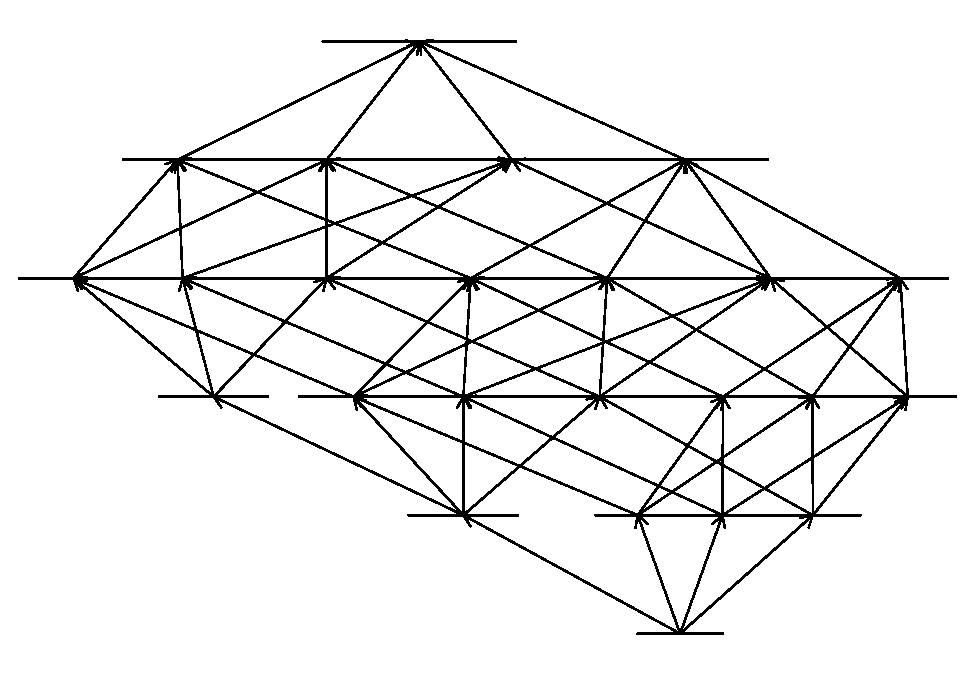
\includegraphics{bookdown-demo_files/figure-latex/unnamed-chunk-11-1.pdf}

In this last plot we can see it's a quite small lattice, and it would require a deeper analysis to extract some conclusions.

\hypertarget{regression}{%
\chapter{Regression}\label{regression}}

\begin{Shaded}
\begin{Highlighting}[]
\KeywordTok{library}\NormalTok{(readxl)}
\KeywordTok{library}\NormalTok{(ggplot2)}
\KeywordTok{library}\NormalTok{(dplyr)}
\KeywordTok{library}\NormalTok{(magrittr)}
\KeywordTok{library}\NormalTok{(ggplot2)}
\KeywordTok{library}\NormalTok{(GGally)}
\end{Highlighting}
\end{Shaded}

We process the dataset to be able to work with it.

\begin{Shaded}
\begin{Highlighting}[]
\KeywordTok{colnames}\NormalTok{(cs) \textless{}{-}}\StringTok{ }\KeywordTok{c}\NormalTok{(}\StringTok{"Fecha"}\NormalTok{, }\StringTok{"Territorio"}\NormalTok{, }\StringTok{"Confirmados\_PCR"}\NormalTok{, }\StringTok{"Hospitalizados"}\NormalTok{, }\StringTok{"UCI"}\NormalTok{, }\StringTok{"Curados"}\NormalTok{, }\StringTok{"Defunciones"}\NormalTok{, }\StringTok{"Total\_confirmados"}\NormalTok{)}
\NormalTok{juntos \textless{}{-}}\StringTok{ }
\StringTok{  }\KeywordTok{filter}\NormalTok{(cs, cs}\OperatorTok{$}\NormalTok{Territorio }\OperatorTok{==}\StringTok{ "Andalucía"}\NormalTok{)}
\NormalTok{juntos \textless{}{-}}\StringTok{ }\KeywordTok{mutate}\NormalTok{(juntos, }\DataTypeTok{Total =} \KeywordTok{cumsum}\NormalTok{(Total\_confirmados))}
                        
                        
\NormalTok{c \textless{}{-}}\StringTok{ }\NormalTok{juntos}\OperatorTok{$}\NormalTok{Curados}
\NormalTok{h \textless{}{-}}\StringTok{ }\NormalTok{juntos}\OperatorTok{$}\NormalTok{Hospitalizados}
\NormalTok{d \textless{}{-}}\StringTok{ }\NormalTok{juntos}\OperatorTok{$}\NormalTok{Defunciones}
\NormalTok{uci \textless{}{-}}\StringTok{ }\NormalTok{juntos}\OperatorTok{$}\NormalTok{UCI}
\NormalTok{conf \textless{}{-}}\StringTok{ }\NormalTok{juntos}\OperatorTok{$}\NormalTok{Confirmados\_PCR}
\NormalTok{totalconf \textless{}{-}}\StringTok{ }\NormalTok{juntos}\OperatorTok{$}\NormalTok{Total\_confirmados}
\NormalTok{salidac \textless{}{-}}\StringTok{ }\KeywordTok{vector}\NormalTok{(}\StringTok{"numeric"}\NormalTok{,}\KeywordTok{length}\NormalTok{(c))}
\NormalTok{salidah \textless{}{-}}\KeywordTok{vector}\NormalTok{(}\StringTok{"numeric"}\NormalTok{,}\KeywordTok{length}\NormalTok{(h))}
\NormalTok{salidad \textless{}{-}}\StringTok{ }\KeywordTok{vector}\NormalTok{(}\StringTok{"numeric"}\NormalTok{,}\KeywordTok{length}\NormalTok{(d))}
\NormalTok{salidauci \textless{}{-}}\StringTok{ }\KeywordTok{vector}\NormalTok{(}\StringTok{"numeric"}\NormalTok{,}\KeywordTok{length}\NormalTok{(uci))}
\NormalTok{salidaconf \textless{}{-}}\StringTok{ }\KeywordTok{vector}\NormalTok{(}\StringTok{"numeric"}\NormalTok{,}\KeywordTok{length}\NormalTok{(conf))}
\NormalTok{salidatotalconf \textless{}{-}}\StringTok{ }\KeywordTok{vector}\NormalTok{(}\StringTok{"numeric"}\NormalTok{,}\KeywordTok{length}\NormalTok{(totalconf))}
\ControlFlowTok{for}\NormalTok{(i }\ControlFlowTok{in} \KeywordTok{seq\_along}\NormalTok{(c))\{}
  
\NormalTok{  salidac[}\KeywordTok{length}\NormalTok{(c)}\OperatorTok{+}\DecValTok{1}\OperatorTok{{-}}\NormalTok{i] \textless{}{-}}\StringTok{ }\NormalTok{c[i]}
\NormalTok{  salidah[}\KeywordTok{length}\NormalTok{(h)}\OperatorTok{+}\DecValTok{1}\OperatorTok{{-}}\NormalTok{i] \textless{}{-}}\StringTok{ }\NormalTok{h[i]}
\NormalTok{  salidad[}\KeywordTok{length}\NormalTok{(d)}\OperatorTok{+}\DecValTok{1}\OperatorTok{{-}}\NormalTok{i] \textless{}{-}}\StringTok{ }\NormalTok{d[i]}
\NormalTok{  salidauci[}\KeywordTok{length}\NormalTok{(uci)}\OperatorTok{+}\DecValTok{1}\OperatorTok{{-}}\NormalTok{i] \textless{}{-}}\StringTok{ }\NormalTok{uci[i]}
\NormalTok{  salidaconf[}\KeywordTok{length}\NormalTok{(conf)}\OperatorTok{+}\DecValTok{1}\OperatorTok{{-}}\NormalTok{i] \textless{}{-}}\StringTok{ }\NormalTok{conf[i]}
\NormalTok{  salidatotalconf[}\KeywordTok{length}\NormalTok{(totalconf)}\OperatorTok{+}\DecValTok{1}\OperatorTok{{-}}\NormalTok{i] \textless{}{-}}\StringTok{ }\NormalTok{totalconf[i]}
  
\NormalTok{\}}
\NormalTok{juntos}\OperatorTok{$}\NormalTok{Curados \textless{}{-}}\StringTok{ }\NormalTok{salidac}
\NormalTok{juntos}\OperatorTok{$}\NormalTok{Hospitalizados \textless{}{-}}\StringTok{ }\NormalTok{salidah}
\NormalTok{juntos}\OperatorTok{$}\NormalTok{Defunciones \textless{}{-}}\StringTok{ }\NormalTok{salidad}
\NormalTok{juntos}\OperatorTok{$}\NormalTok{UCI \textless{}{-}}\StringTok{ }\NormalTok{salidauci}
\NormalTok{juntos}\OperatorTok{$}\NormalTok{Confirmados\_PCR \textless{}{-}}\StringTok{ }\NormalTok{salidaconf}
\NormalTok{juntos}\OperatorTok{$}\NormalTok{Total\_confirmados \textless{}{-}}\StringTok{ }\NormalTok{salidatotalconf}
                     
\NormalTok{  fechas \textless{}{-}}\StringTok{ }\KeywordTok{as.Date}\NormalTok{(juntos}\OperatorTok{$}\NormalTok{Fecha ,}\StringTok{"\%d/\%m/\%Y"}\NormalTok{)}
\NormalTok{juntos}\OperatorTok{$}\NormalTok{Fecha \textless{}{-}}\StringTok{ }\KeywordTok{sort}\NormalTok{(fechas)                      }
\end{Highlighting}
\end{Shaded}

We make the graph of how the cases have increased as a function of time.

\begin{Shaded}
\begin{Highlighting}[]
\KeywordTok{attach}\NormalTok{(juntos)}
\end{Highlighting}
\end{Shaded}

\begin{verbatim}
## The following objects are masked from juntos (pos = 3):
## 
##     Confirmados_PCR, Curados, Defunciones, Fecha, Hospitalizados,
##     Territorio, Total, Total_confirmados, UCI
\end{verbatim}

\begin{Shaded}
\begin{Highlighting}[]
\NormalTok{grafica \textless{}{-}}\StringTok{ }\NormalTok{juntos }\OperatorTok{\%\textgreater{}\%}\StringTok{ }\KeywordTok{ggplot}\NormalTok{(}\KeywordTok{aes}\NormalTok{(}\DataTypeTok{x=}\NormalTok{ Fecha, }\DataTypeTok{y=}\NormalTok{ Total))}\OperatorTok{+}\KeywordTok{geom\_point}\NormalTok{()}
\NormalTok{grafica}
\end{Highlighting}
\end{Shaded}

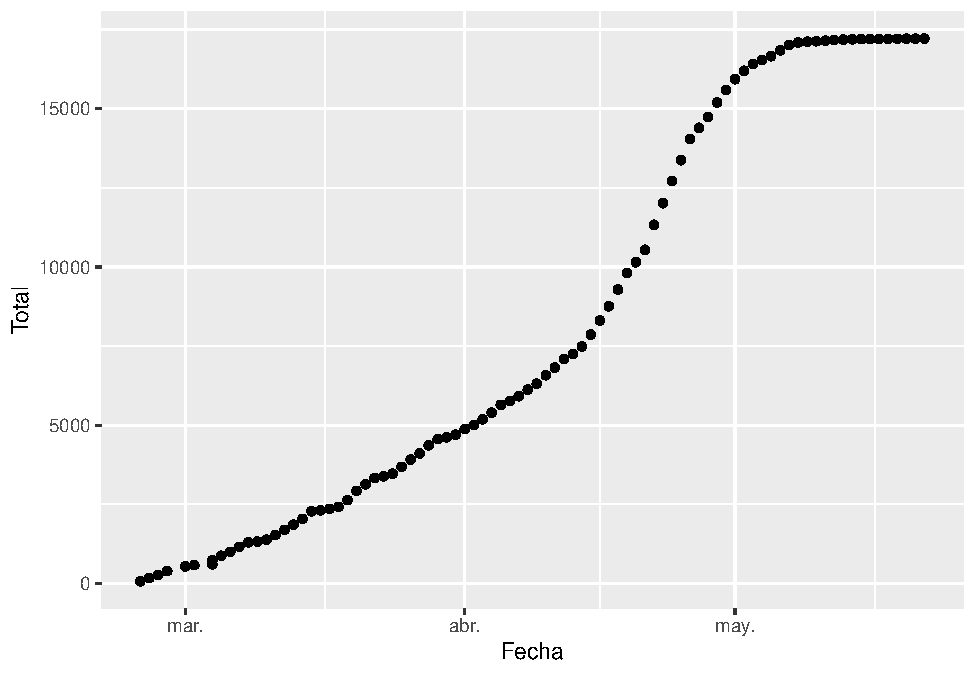
\includegraphics{bookdown-demo_files/figure-latex/unnamed-chunk-15-1.pdf}

In this graph we can see how the number of cases up to May increased exponentially. However, starting from this date, the number of cases per day begins to decrease, reaching the famous peak.

\hypertarget{model-of-the-number-of-infections-with-respect-to-the-date}{%
\section{Model of the number of infections with respect to the date}\label{model-of-the-number-of-infections-with-respect-to-the-date}}

\begin{Shaded}
\begin{Highlighting}[]
\NormalTok{modFC \textless{}{-}}\StringTok{ }\KeywordTok{lm}\NormalTok{(}\DataTypeTok{formula =}\NormalTok{ juntos}\OperatorTok{$}\NormalTok{Total }\OperatorTok{\textasciitilde{}}\StringTok{ }\NormalTok{juntos}\OperatorTok{$}\NormalTok{Fecha, }\DataTypeTok{data =}\NormalTok{ juntos)}
\NormalTok{modFC}
\end{Highlighting}
\end{Shaded}

\begin{verbatim}
## 
## Call:
## lm(formula = juntos$Total ~ juntos$Fecha, data = juntos)
## 
## Coefficients:
##  (Intercept)  juntos$Fecha  
##   -4444803.2         242.5
\end{verbatim}

\begin{Shaded}
\begin{Highlighting}[]
\KeywordTok{summary}\NormalTok{(modFC)}
\end{Highlighting}
\end{Shaded}

\begin{verbatim}
## 
## Call:
## lm(formula = juntos$Total ~ juntos$Fecha, data = juntos)
## 
## Residuals:
##     Min      1Q  Median      3Q     Max 
## -2038.5 -1147.8  -133.7  1165.0  2423.5 
## 
## Coefficients:
##                Estimate Std. Error t value Pr(>|t|)    
## (Intercept)  -4.445e+06  1.110e+05  -40.03   <2e-16 ***
## juntos$Fecha  2.425e+02  6.047e+00   40.11   <2e-16 ***
## ---
## Signif. codes:  0 '***' 0.001 '**' 0.01 '*' 0.05 '.' 0.1 ' ' 1
## 
## Residual standard error: 1420 on 85 degrees of freedom
## Multiple R-squared:  0.9498, Adjusted R-squared:  0.9492 
## F-statistic:  1609 on 1 and 85 DF,  p-value: < 2.2e-16
\end{verbatim}

We start by checking if there is a model, for this we look at the values of F-statistic and p-value.
** F-statistic ** is quite far from 1 (1609), so it indicates that there is a model.
** P-value **, is well below 0.005, confirming that there is a model (H1 is met)
Now that we know there is a model, let's study how good our model is.

We look at \(R^2\), which has a value of 0.9498, a pretty good value, since \textbf{94.98\%} of the cases are collected with this model.
We also see that there is almost no difference between adjusted \(R^2\) and \(R^2\), so \emph{there is no overfitting} in our model and that the values are relevant (indicated by ***)
Let's continue studying the model, for this we will see the graphs of the adjusted values and residuals.

\begin{Shaded}
\begin{Highlighting}[]
\KeywordTok{plot}\NormalTok{(modFC)}
\end{Highlighting}
\end{Shaded}

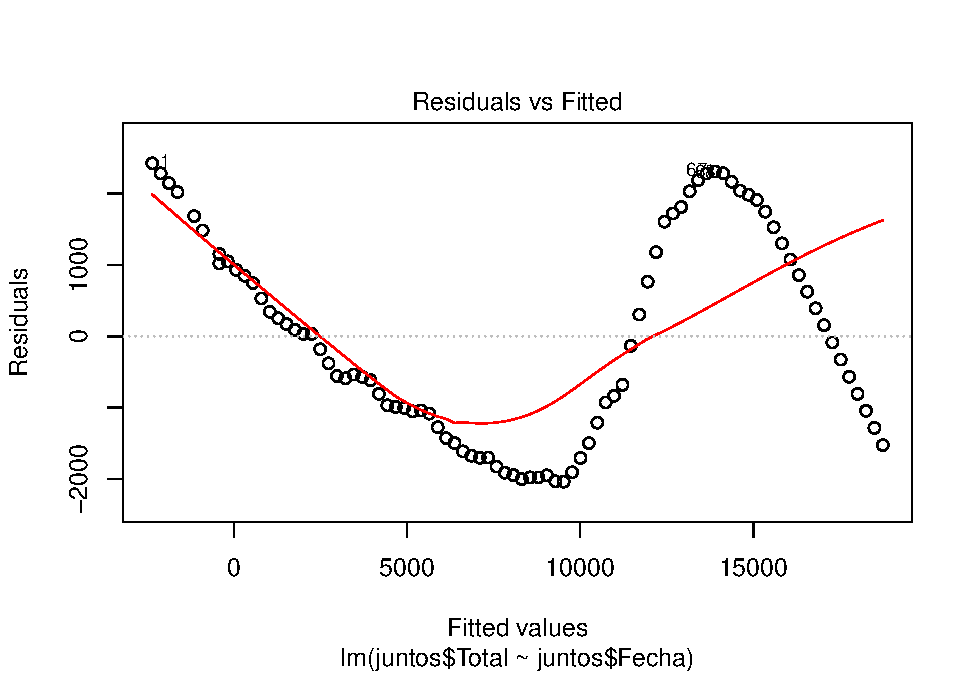
\includegraphics{bookdown-demo_files/figure-latex/unnamed-chunk-18-1.pdf} 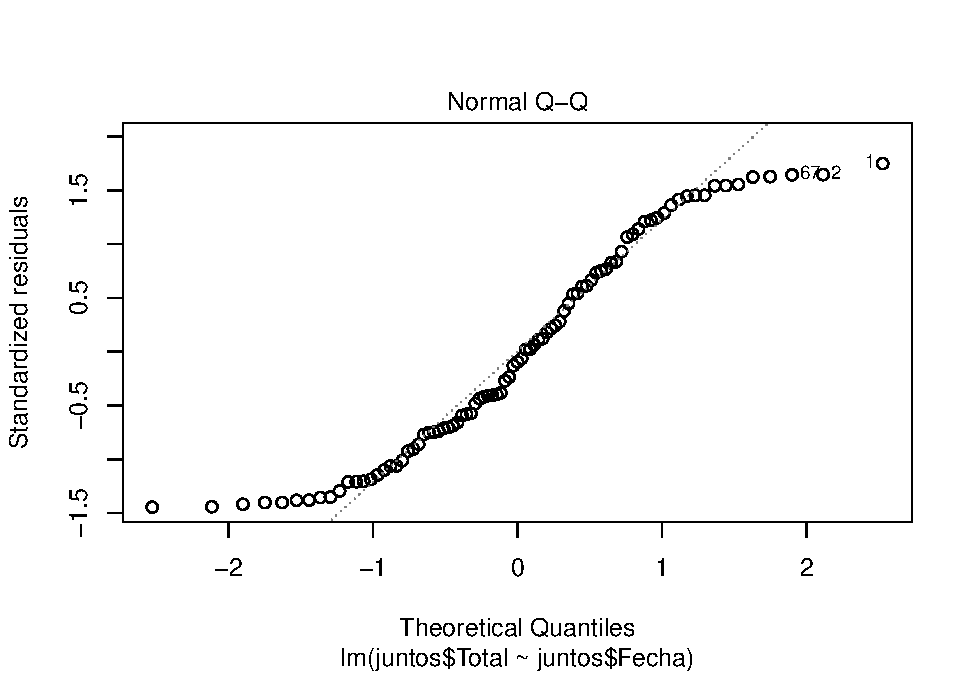
\includegraphics{bookdown-demo_files/figure-latex/unnamed-chunk-18-2.pdf} 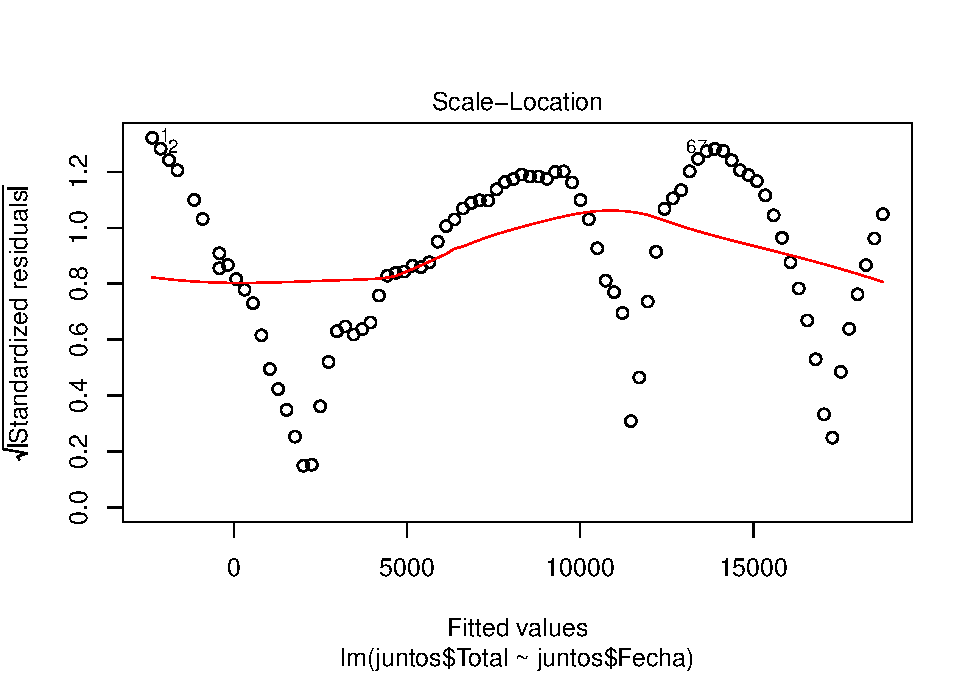
\includegraphics{bookdown-demo_files/figure-latex/unnamed-chunk-18-3.pdf} 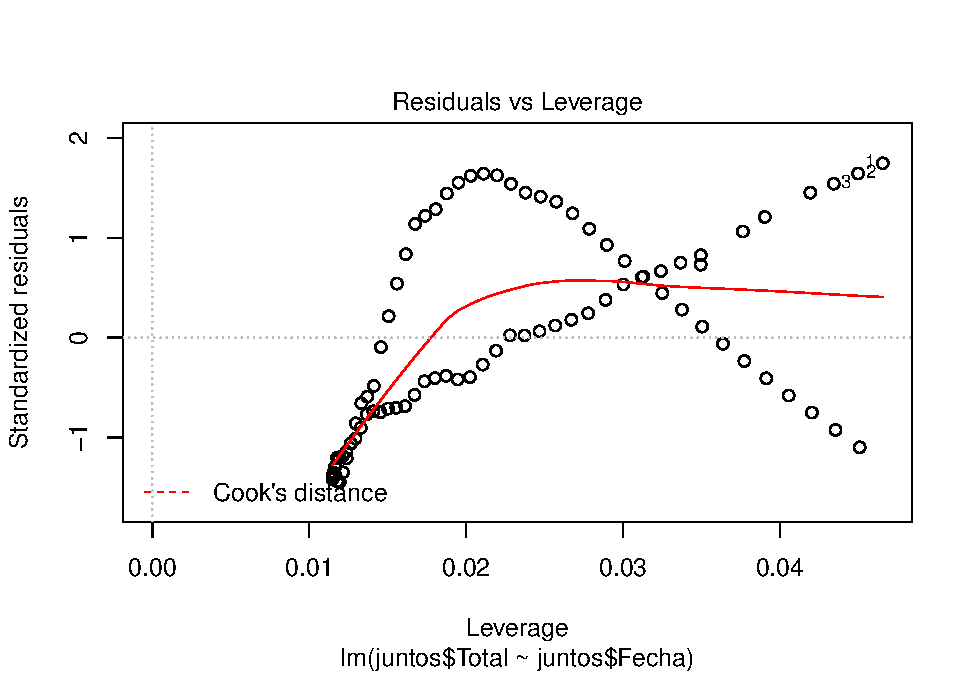
\includegraphics{bookdown-demo_files/figure-latex/unnamed-chunk-18-4.pdf}

In these graphs we can see how it begins adjusting to the values. However, as cases increase, there is more waste.
This may be due to the results of the contingency measures that were taken.
With all this we could say that we have a pretty good model.
\#\# Model of the number of people who were hospitalized with respect to the number of infected.

\begin{Shaded}
\begin{Highlighting}[]
\NormalTok{mHospitalizados \textless{}{-}}\StringTok{ }\KeywordTok{lm}\NormalTok{(}\DataTypeTok{formula =}\NormalTok{ Hospitalizados }\OperatorTok{\textasciitilde{}}\StringTok{ }\NormalTok{Total\_confirmados, }\DataTypeTok{data =}\NormalTok{ juntos)}
\NormalTok{mHospitalizados}
\end{Highlighting}
\end{Shaded}

\begin{verbatim}
## 
## Call:
## lm(formula = Hospitalizados ~ Total_confirmados, data = juntos)
## 
## Coefficients:
##       (Intercept)  Total_confirmados  
##          -31.5285             0.5212
\end{verbatim}

\begin{Shaded}
\begin{Highlighting}[]
\KeywordTok{summary}\NormalTok{(mHospitalizados)}
\end{Highlighting}
\end{Shaded}

\begin{verbatim}
## 
## Call:
## lm(formula = Hospitalizados ~ Total_confirmados, data = juntos)
## 
## Residuals:
##     Min      1Q  Median      3Q     Max 
## -98.696 -24.055   4.173  29.359  84.144 
## 
## Coefficients:
##                    Estimate Std. Error t value Pr(>|t|)    
## (Intercept)       -31.52846    5.98438  -5.268 1.02e-06 ***
## Total_confirmados   0.52117    0.02246  23.200  < 2e-16 ***
## ---
## Signif. codes:  0 '***' 0.001 '**' 0.01 '*' 0.05 '.' 0.1 ' ' 1
## 
## Residual standard error: 37.37 on 85 degrees of freedom
## Multiple R-squared:  0.8636, Adjusted R-squared:  0.862 
## F-statistic: 538.3 on 1 and 85 DF,  p-value: < 2.2e-16
\end{verbatim}

We start by checking if there is a model, for this we look at the values of F-statistic and p-value.
F-statistic is quite far from 1 (538), so it indicates that there is a model.
P-value, is well below 0.005, which confirms that there is a model (H1 is met)
Now that we know there is a model, let's study how good our model is.
We look at \(R^2\), which has a value of 0.8636, a pretty good value, since 86.36\% of hospitalization cases are included in this model.
We also see that there is almost no difference between adjusted \(R^2\) and \(R^2\), so there is no overfitting in our model and that the values are relevant (indicated by ***)
Let's continue studying the model, for this we will see the graphs of the adjusted values and residuals.

\begin{Shaded}
\begin{Highlighting}[]
\KeywordTok{plot}\NormalTok{(mHospitalizados)}
\end{Highlighting}
\end{Shaded}

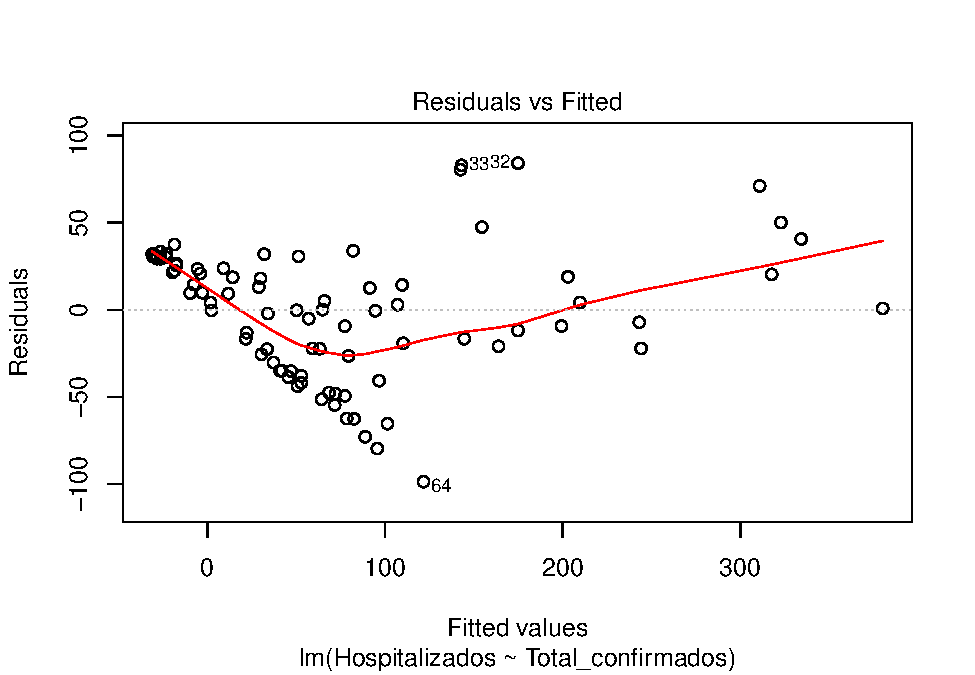
\includegraphics{bookdown-demo_files/figure-latex/unnamed-chunk-21-1.pdf} 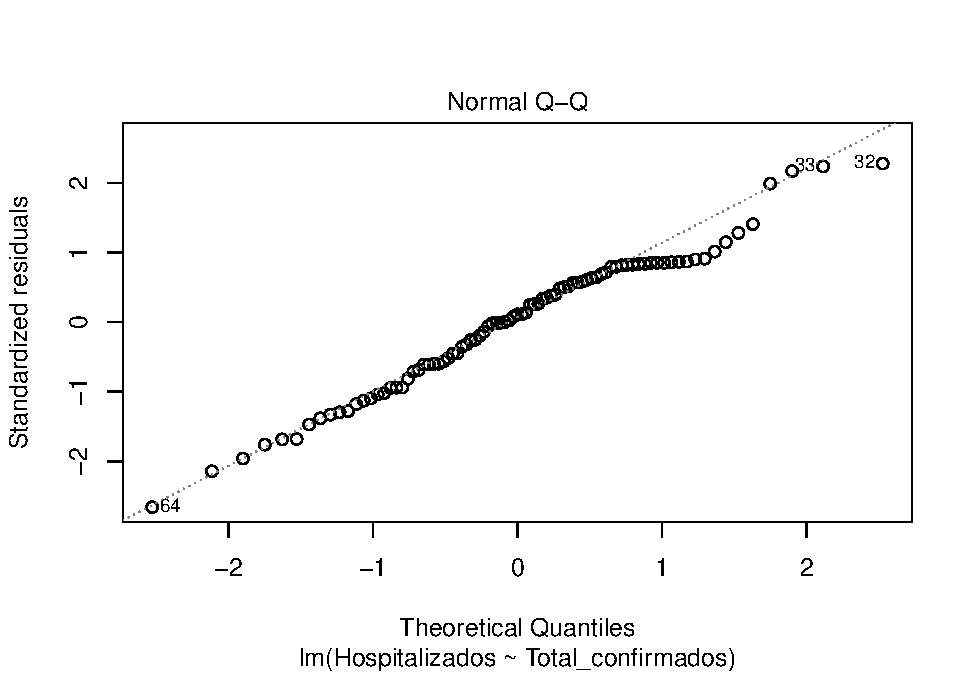
\includegraphics{bookdown-demo_files/figure-latex/unnamed-chunk-21-2.pdf} 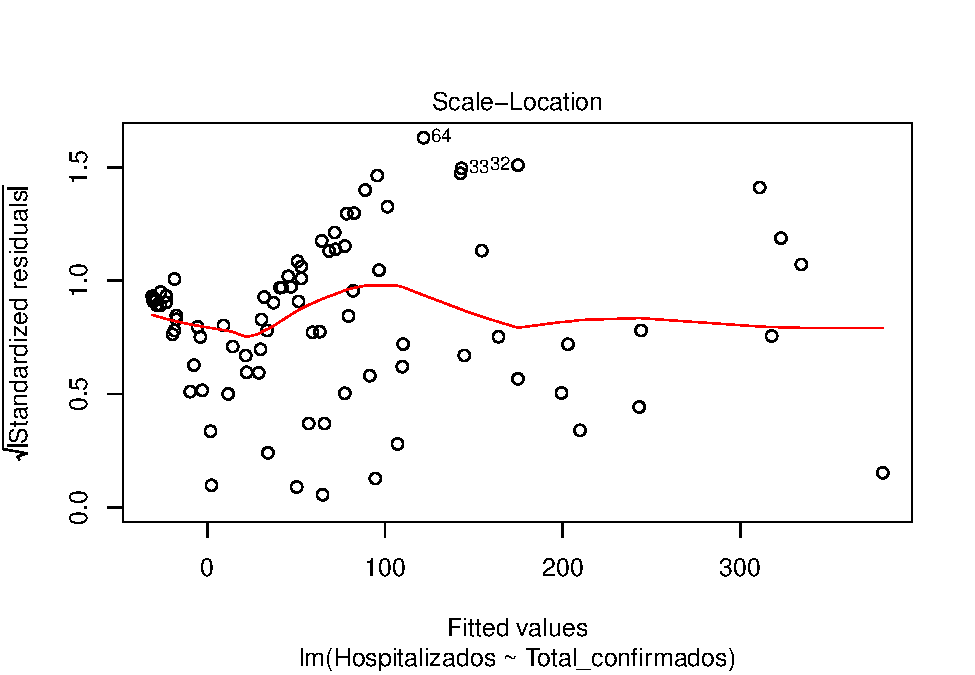
\includegraphics{bookdown-demo_files/figure-latex/unnamed-chunk-21-3.pdf} 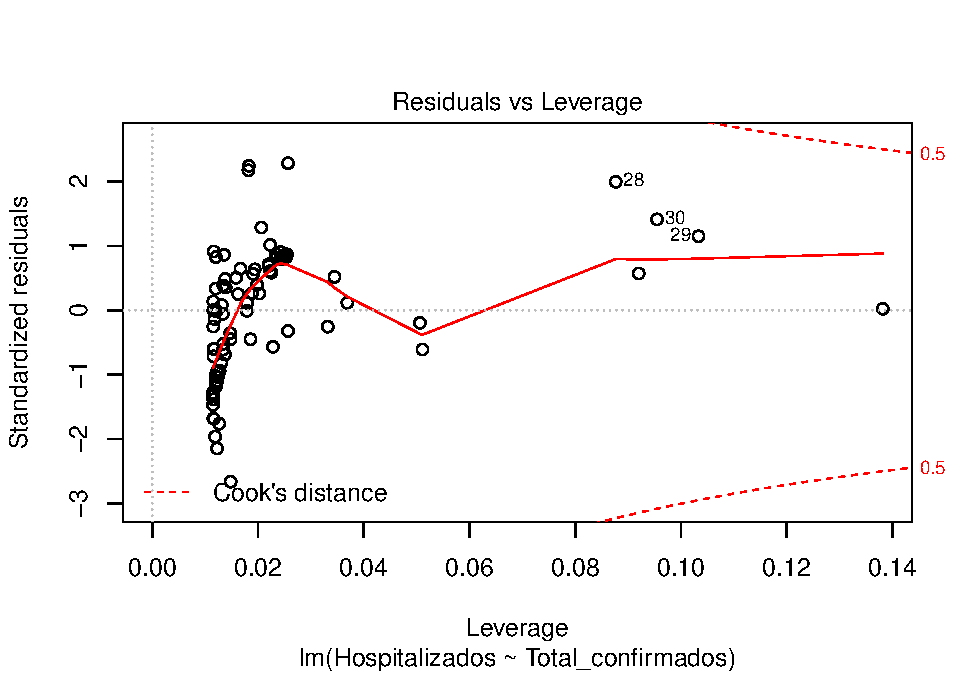
\includegraphics{bookdown-demo_files/figure-latex/unnamed-chunk-21-4.pdf}

In the graphs we can see how there is dispersion of the values, and how it fits better at the beginning than at the end.
We also observed that at the beginning of the period the number of hospitalized was very close to the number of cases. But as time progresses, the number of cases increases considerably, but not so much the number of hospitalized. This may be due to the fact that the population was informed of the first symptoms and the measures they had to take, so that an infected person could be detected in the early stages and monitored so that the severity could be reduced.

\begin{Shaded}
\begin{Highlighting}[]
\KeywordTok{library}\NormalTok{(readxl)}
\KeywordTok{library}\NormalTok{(tidyverse)}
\NormalTok{datos \textless{}{-}}\StringTok{ }\KeywordTok{read\_excel}\NormalTok{(}\StringTok{"cs\_export.xls"}\NormalTok{)}
\NormalTok{datos \textless{}{-}}\StringTok{ }\KeywordTok{na.omit}\NormalTok{(datos)}
\KeywordTok{names}\NormalTok{(datos) \textless{}{-}}\StringTok{ }\KeywordTok{c}\NormalTok{(}\KeywordTok{names}\NormalTok{(datos[}\DecValTok{1}\OperatorTok{:}\DecValTok{2}\NormalTok{]),}\StringTok{"Confirmados\_PCR"}\NormalTok{,}\KeywordTok{names}\NormalTok{(datos[}\DecValTok{4}\OperatorTok{:}\DecValTok{7}\NormalTok{]),}\StringTok{"Total\_confirmados"}\NormalTok{)}
\NormalTok{varPred \textless{}{-}}\StringTok{ }\KeywordTok{names}\NormalTok{(datos[}\KeywordTok{c}\NormalTok{(}\DecValTok{3}\OperatorTok{:}\DecValTok{6}\NormalTok{,}\DecValTok{8}\NormalTok{)])}
\NormalTok{datos}\OperatorTok{$}\StringTok{\textasciigrave{}}\DataTypeTok{Fecha declaración}\StringTok{\textasciigrave{}}\NormalTok{ \textless{}{-}}\StringTok{ }\KeywordTok{as.Date}\NormalTok{(datos}\OperatorTok{$}\StringTok{\textasciigrave{}}\DataTypeTok{Fecha declaración}\StringTok{\textasciigrave{}}\NormalTok{, }\StringTok{"\%d/\%m/\%Y"}\NormalTok{)}
\NormalTok{datos \textless{}{-}}\StringTok{ }\KeywordTok{arrange}\NormalTok{(datos, }\StringTok{\textasciigrave{}}\DataTypeTok{Fecha declaración}\StringTok{\textasciigrave{}}\NormalTok{)}
\NormalTok{filasandalucia \textless{}{-}}\StringTok{ }\KeywordTok{filter}\NormalTok{(datos, Territorio}\OperatorTok{==}\StringTok{"Andalucía"}\NormalTok{ )}
\end{Highlighting}
\end{Shaded}

We are going to produce a multivariate regression model that explains the variable \emph{Defunction} using an iterative technique in which we will add each time the variable whose R-adjusted is greater.

We define a function to calculate the linear model of a sum of variables

\begin{Shaded}
\begin{Highlighting}[]
\NormalTok{linearAdjust \textless{}{-}}\StringTok{ }\ControlFlowTok{function}\NormalTok{(df, y, x)\{}
\NormalTok{  mod1 \textless{}{-}}\StringTok{ }\KeywordTok{lm}\NormalTok{(}\KeywordTok{str\_c}\NormalTok{(y,}\StringTok{"\textasciitilde{}"}\NormalTok{,}\KeywordTok{str\_c}\NormalTok{(x,}\DataTypeTok{collapse=}\StringTok{"+"}\NormalTok{)),df)}
\NormalTok{\}}
\NormalTok{calcModR2 \textless{}{-}}\StringTok{ }\ControlFlowTok{function}\NormalTok{(df,y,x)\{}
\NormalTok{  mod \textless{}{-}}\StringTok{ }\KeywordTok{linearAdjust}\NormalTok{(df,y,x)}
  \KeywordTok{summary}\NormalTok{(mod)}\OperatorTok{$}\NormalTok{adj.r.squared}
\NormalTok{\}}
\end{Highlighting}
\end{Shaded}

We are adding variables while increasing the value of adjusted \(R^2\).

\begin{Shaded}
\begin{Highlighting}[]
\NormalTok{encontrarMejorAjuste \textless{}{-}}\StringTok{ }\ControlFlowTok{function}\NormalTok{(df,varPos)\{}
\NormalTok{  bestVars \textless{}{-}}\StringTok{ }\KeywordTok{character}\NormalTok{(}\DecValTok{0}\NormalTok{)}
\NormalTok{  aR2 \textless{}{-}}\StringTok{ }\DecValTok{0}
  \ControlFlowTok{repeat}\NormalTok{\{}
\NormalTok{    aR2v \textless{}{-}}\StringTok{ }\KeywordTok{map\_dbl}\NormalTok{(varPos,}\OperatorTok{\textasciitilde{}}\KeywordTok{calcModR2}\NormalTok{(df, }\StringTok{"Defunciones"}\NormalTok{,}\KeywordTok{c}\NormalTok{(bestVars,.)))}
\NormalTok{    i    \textless{}{-}}\StringTok{ }\KeywordTok{which.max}\NormalTok{(aR2v)}
\NormalTok{    aR2M \textless{}{-}}\StringTok{ }\NormalTok{aR2v[i]}
    
    \ControlFlowTok{if}\NormalTok{(aR2M}\OperatorTok{\textless{}=}\NormalTok{aR2 }\OperatorTok{||}\KeywordTok{length}\NormalTok{(varPos)}\OperatorTok{\textless{}}\DecValTok{1}\NormalTok{) }\ControlFlowTok{break}
    \CommentTok{\#Valor del r{-}ajustado añadido y nombre de la variable elegida}
    \KeywordTok{cat}\NormalTok{(}\KeywordTok{sprintf}\NormalTok{(}\StringTok{"\%1.4f \%s}\CharTok{\textbackslash{}n}\StringTok{"}\NormalTok{,aR2M,varPos[i]))}
\NormalTok{    aR2 \textless{}{-}}\StringTok{ }\NormalTok{aR2M}
\NormalTok{    bestVars \textless{}{-}}\StringTok{ }\KeywordTok{c}\NormalTok{(bestVars,varPos[i])}
\NormalTok{    varPos \textless{}{-}}\StringTok{ }\NormalTok{varPos[}\OperatorTok{{-}}\NormalTok{i]}
\NormalTok{  \}}
\NormalTok{  mod \textless{}{-}}\StringTok{ }\KeywordTok{linearAdjust}\NormalTok{(df,}\StringTok{"Defunciones"}\NormalTok{,bestVars)}
  \KeywordTok{list}\NormalTok{(}\DataTypeTok{vars=}\NormalTok{bestVars,}\DataTypeTok{mod=}\NormalTok{mod)}
\NormalTok{\}}
\NormalTok{bestMod \textless{}{-}}\StringTok{ }\KeywordTok{encontrarMejorAjuste}\NormalTok{(filasandalucia, varPred)}
\end{Highlighting}
\end{Shaded}

\begin{verbatim}
## 0.9499 Hospitalizados
## 0.9521 UCI
## 0.9530 Curados
## 0.9566 Total_confirmados
## 0.9642 Confirmados_PCR
\end{verbatim}

\begin{Shaded}
\begin{Highlighting}[]
\NormalTok{bestMod}
\end{Highlighting}
\end{Shaded}

\begin{verbatim}
## $vars
## [1] "Hospitalizados"    "UCI"               "Curados"          
## [4] "Total_confirmados" "Confirmados_PCR"  
## 
## $mod
## 
## Call:
## lm(formula = str_c(y, "~", str_c(x, collapse = "+")), data = df)
## 
## Coefficients:
##       (Intercept)     Hospitalizados                UCI            Curados  
##           0.26562            0.11219            0.35878           -0.21053  
## Total_confirmados    Confirmados_PCR  
##           0.10853            0.08473
\end{verbatim}

\begin{Shaded}
\begin{Highlighting}[]
\KeywordTok{summary}\NormalTok{(bestMod}\OperatorTok{$}\NormalTok{mod)}
\end{Highlighting}
\end{Shaded}

\begin{verbatim}
## 
## Call:
## lm(formula = str_c(y, "~", str_c(x, collapse = "+")), data = df)
## 
## Residuals:
##      Min       1Q   Median       3Q      Max 
## -11.2602  -2.2208  -0.3433   1.8867  13.9259 
## 
## Coefficients:
##                   Estimate Std. Error t value Pr(>|t|)    
## (Intercept)        0.26562    0.82376   0.322 0.747941    
## Hospitalizados     0.11219    0.03151   3.561 0.000623 ***
## UCI                0.35878    0.10317   3.478 0.000816 ***
## Curados           -0.21053    0.03937  -5.347 8.07e-07 ***
## Total_confirmados  0.10853    0.02412   4.499 2.26e-05 ***
## Confirmados_PCR    0.08473    0.01978   4.284 5.02e-05 ***
## ---
## Signif. codes:  0 '***' 0.001 '**' 0.01 '*' 0.05 '.' 0.1 ' ' 1
## 
## Residual standard error: 4.285 on 81 degrees of freedom
## Multiple R-squared:  0.9663, Adjusted R-squared:  0.9642 
## F-statistic: 463.9 on 5 and 81 DF,  p-value: < 2.2e-16
\end{verbatim}

The model obtained would be of the form:

\[
Defunciones=0.2656235 +0.1121855·Hospitalizados+0.3587845·UCI+-0.2105297·ConfirmadosPCR+0.1085301·Curados+0.0847283·TotalConfirmados
\]

Finally we can represent the graph of the data (purple) with the regression obtained superimposed (red)

\begin{Shaded}
\begin{Highlighting}[]
\NormalTok{g \textless{}{-}}\StringTok{ }\KeywordTok{ggplot}\NormalTok{(filasandalucia, }\KeywordTok{aes}\NormalTok{(}\DataTypeTok{x=}\StringTok{\textasciigrave{}}\DataTypeTok{Fecha declaración}\StringTok{\textasciigrave{}}\NormalTok{,}\DataTypeTok{y=}\NormalTok{Defunciones))}\OperatorTok{+}
\StringTok{  }\KeywordTok{ggtitle}\NormalTok{(}\StringTok{"Regresión multilineal"}\NormalTok{)}\OperatorTok{+}
\StringTok{  }\KeywordTok{geom\_point}\NormalTok{(}\DataTypeTok{colour=}\StringTok{"purple"}\NormalTok{)}\OperatorTok{+}
\StringTok{  }\KeywordTok{geom\_line}\NormalTok{(}\KeywordTok{aes}\NormalTok{(}\StringTok{\textasciigrave{}}\DataTypeTok{Fecha declaración}\StringTok{\textasciigrave{}}\NormalTok{, }\KeywordTok{predict.lm}\NormalTok{(bestMod}\OperatorTok{$}\NormalTok{mod)), }\DataTypeTok{color=}\StringTok{"red"}\NormalTok{)}
  
\NormalTok{g}
\end{Highlighting}
\end{Shaded}

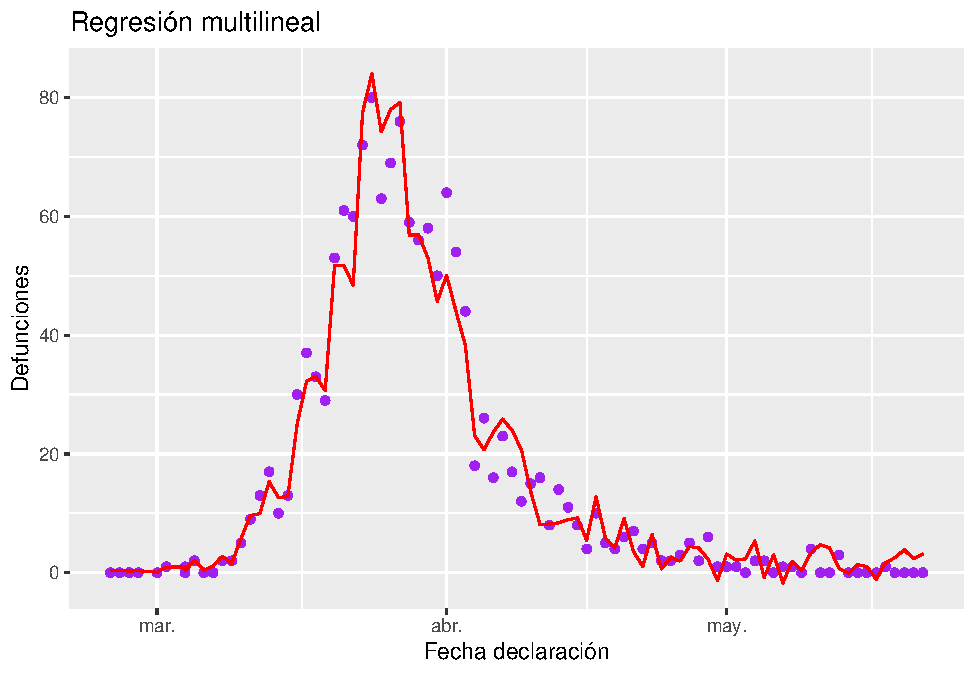
\includegraphics{bookdown-demo_files/figure-latex/unnamed-chunk-26-1.pdf}

\hypertarget{final-words}{%
\chapter{Final Words}\label{final-words}}

As shown thorugh this book, we can find several approaches to analyze the same dataset. Some of them might work and show interesting results, but others might show nothing interesting - and even sometimes nothing at all!

  \bibliography{book.bib,packages.bib}

\end{document}
